% !TEX root = thesis-en.tex
\section{Core Code of the Unity Project File}
\begin{figure}[h]
\centering
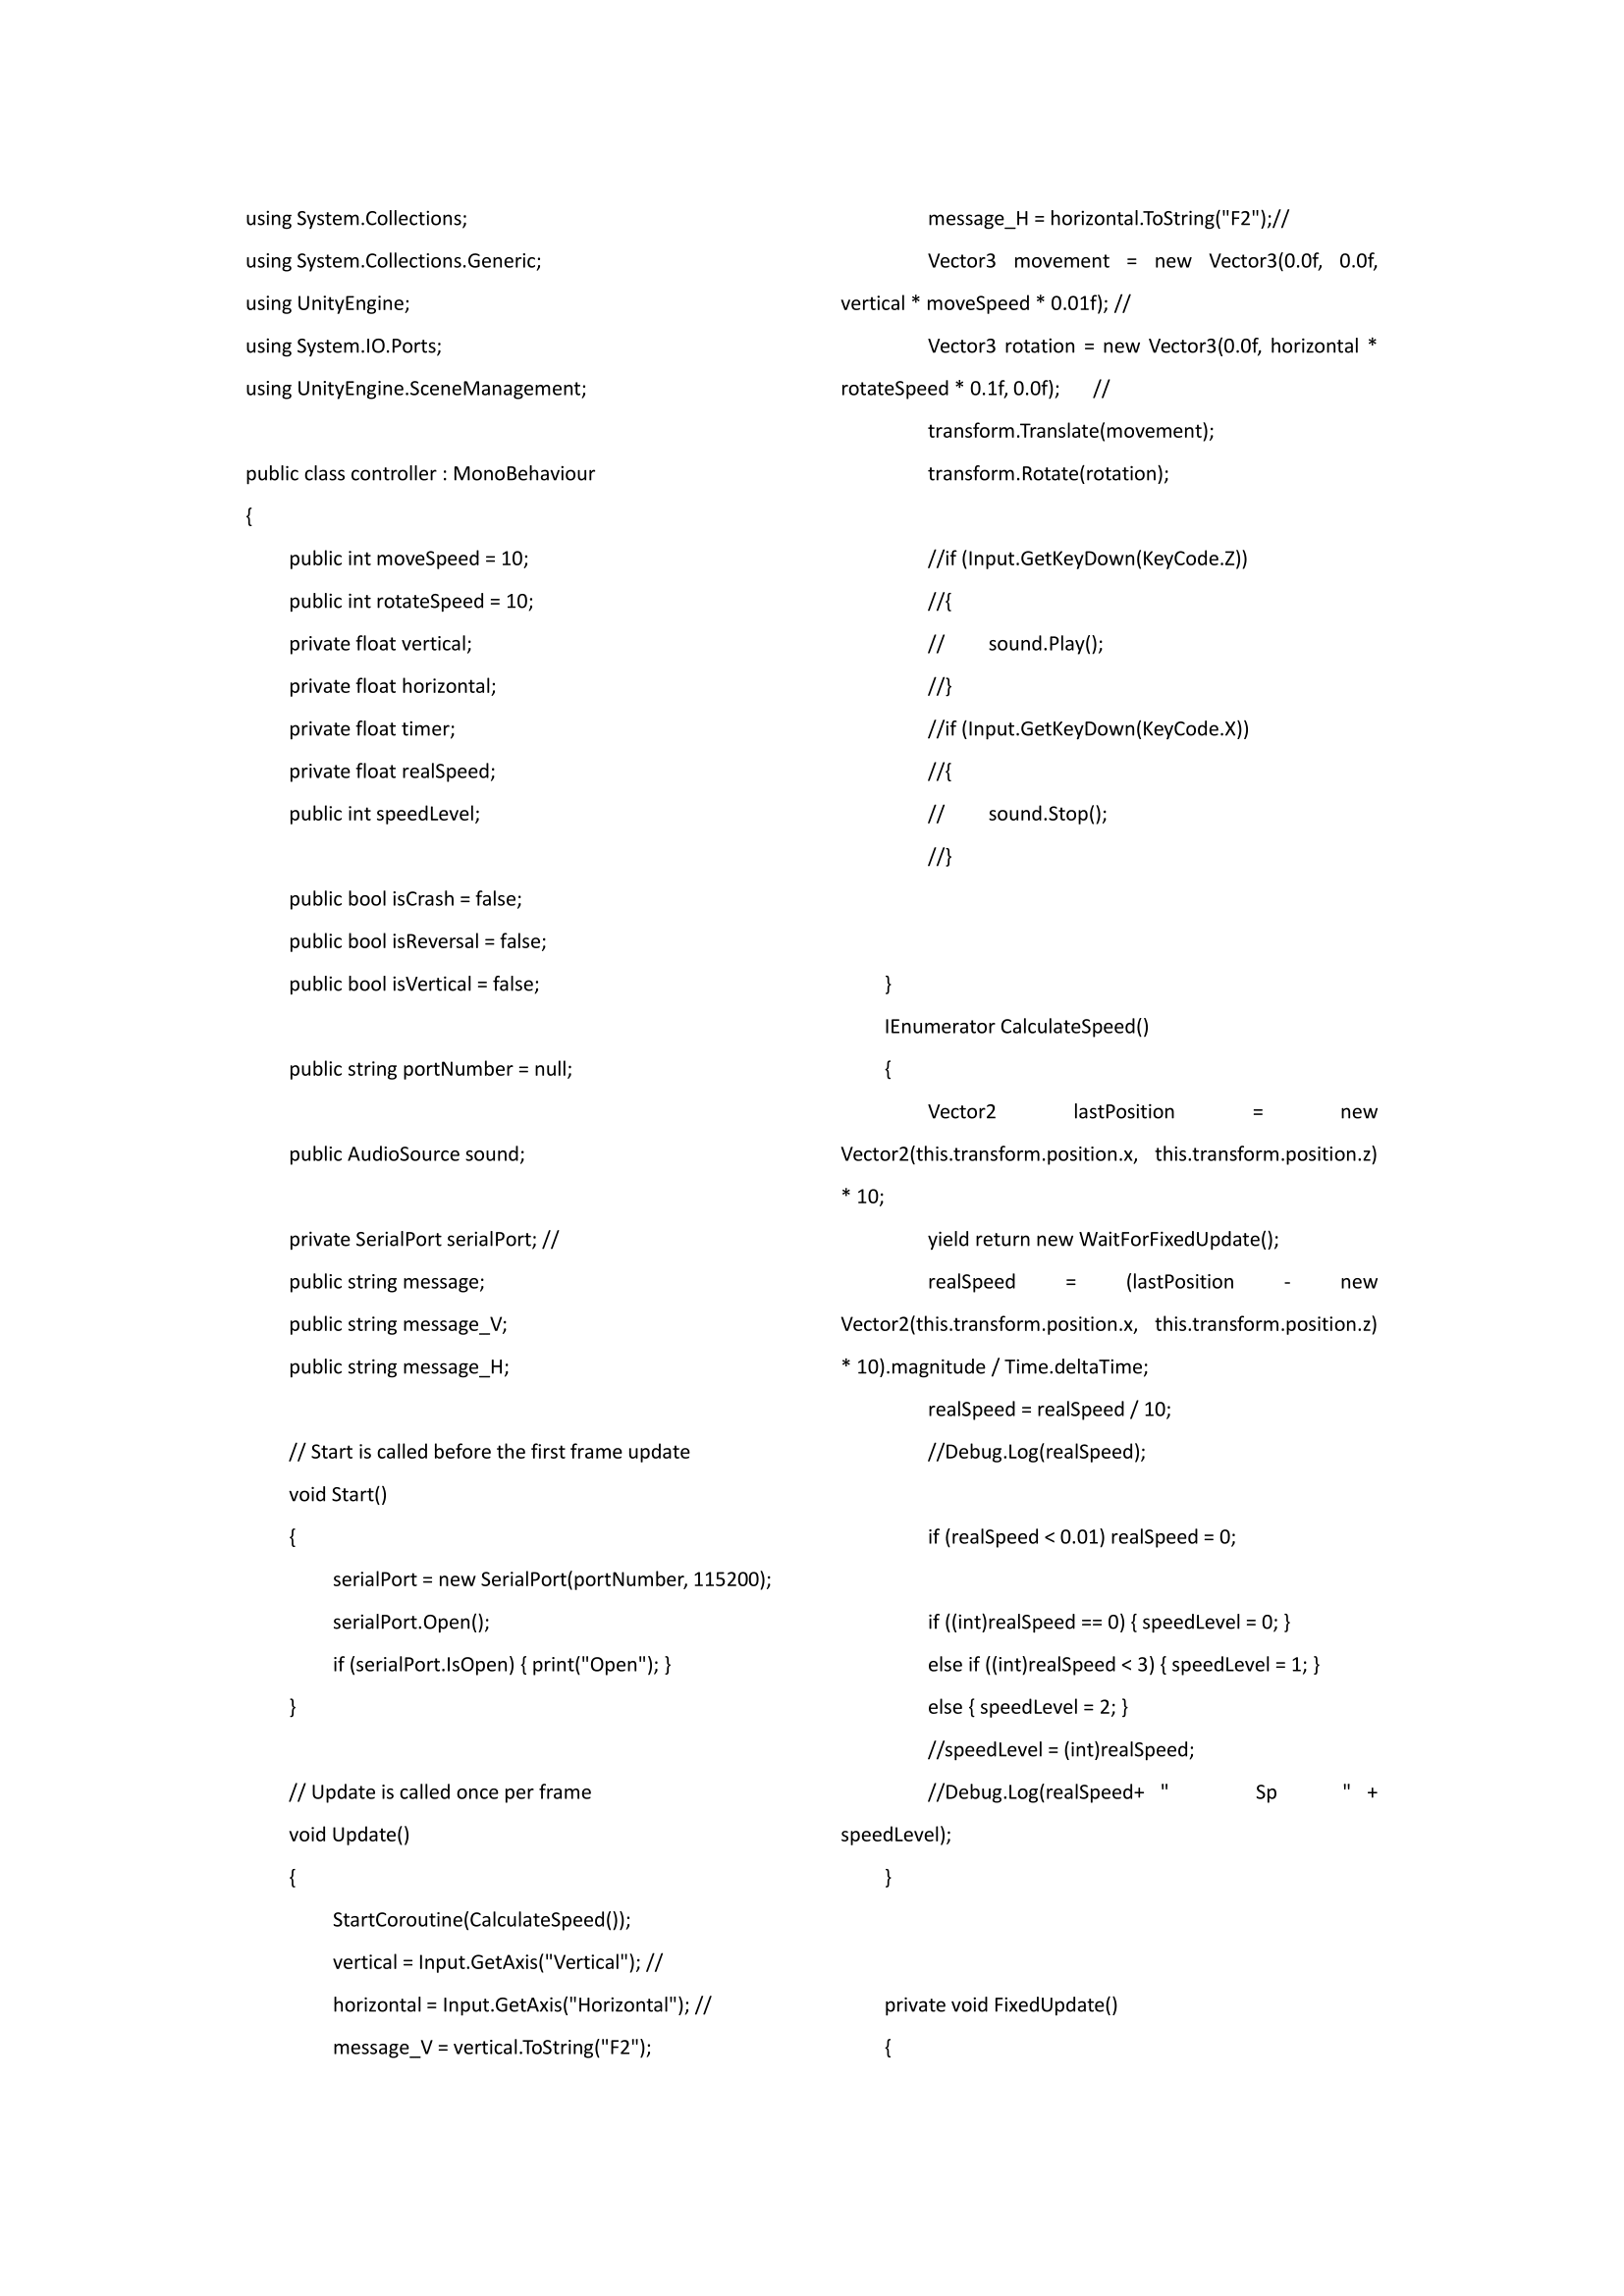
\includegraphics[width=1\textwidth,height=0.7\textheight]{A_thesis/appendix/code_unity-1.png}
\end{figure}
\newpage

\begin{figure}[h]
\centering
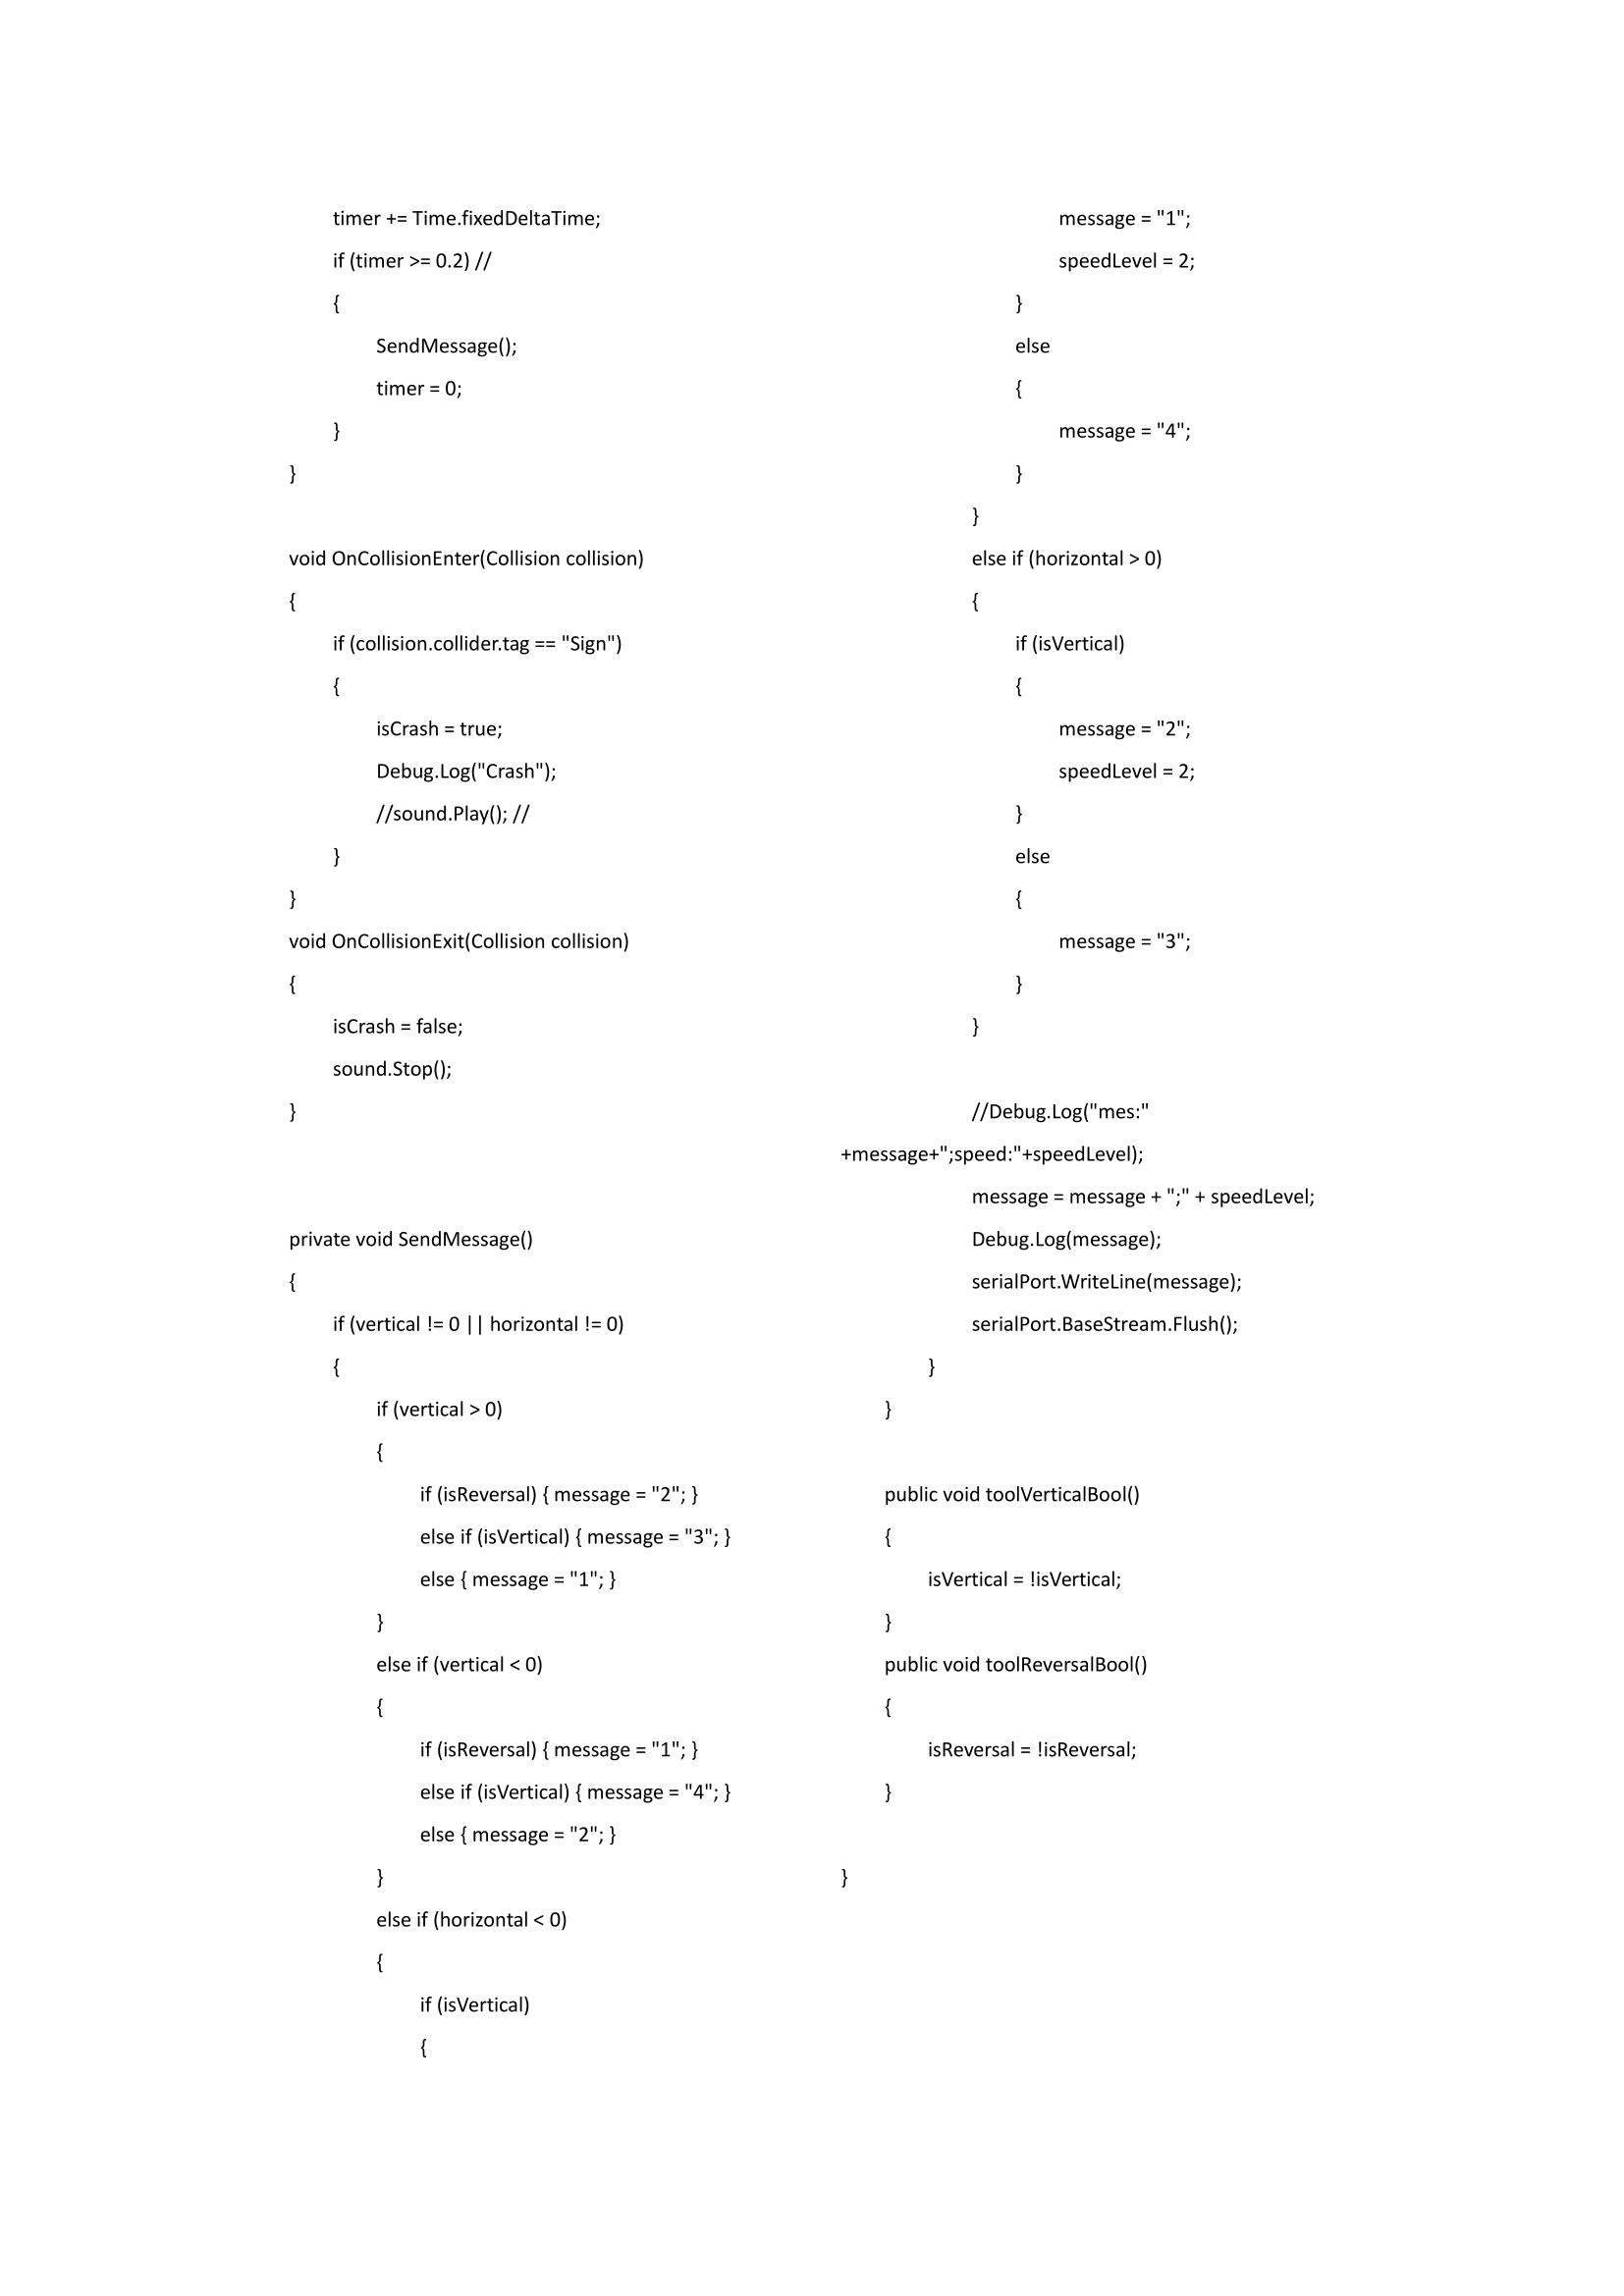
\includegraphics[width=1\textwidth,height=0.7\textheight]{A_thesis/appendix/code_unity-2.png}
\end{figure}
\newpage

\section{Core Code of the Arduino Project File}
\begin{figure}[h]
\centering
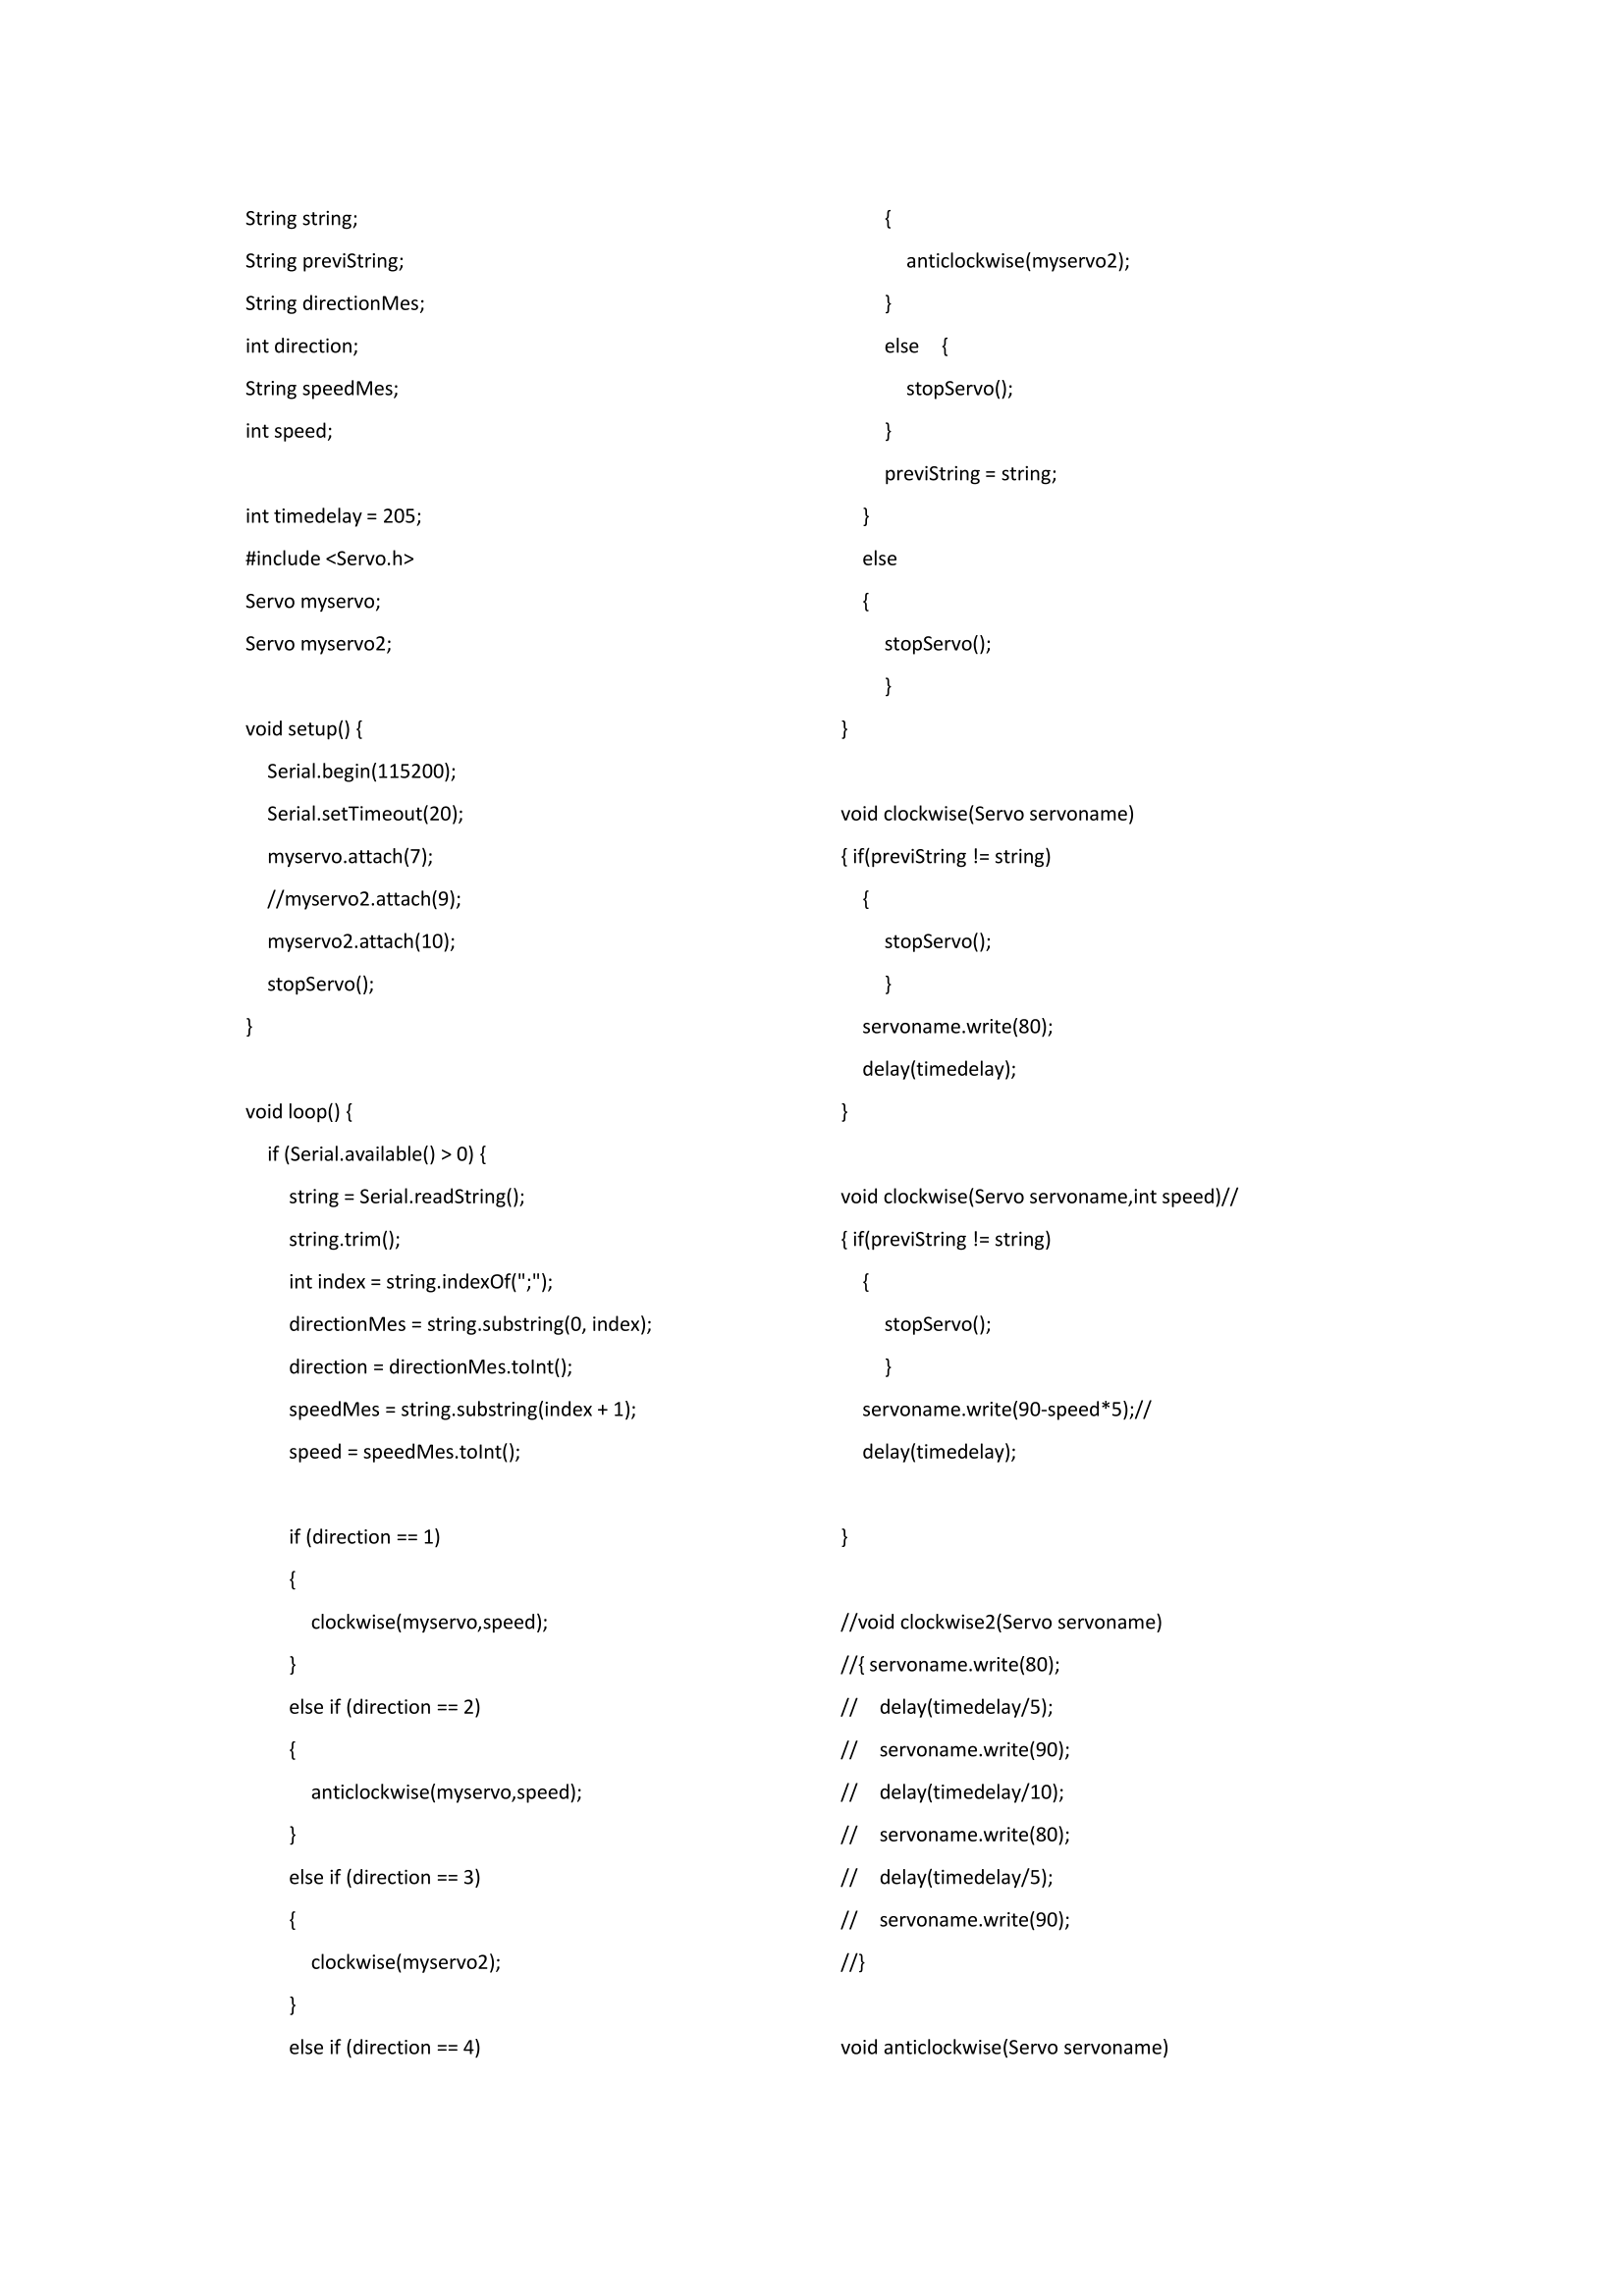
\includegraphics[width=1\textwidth,height=0.7\textheight]{A_thesis/appendix/code_arduino-1.png}
\end{figure}
\newpage

\begin{figure}[h]
\centering
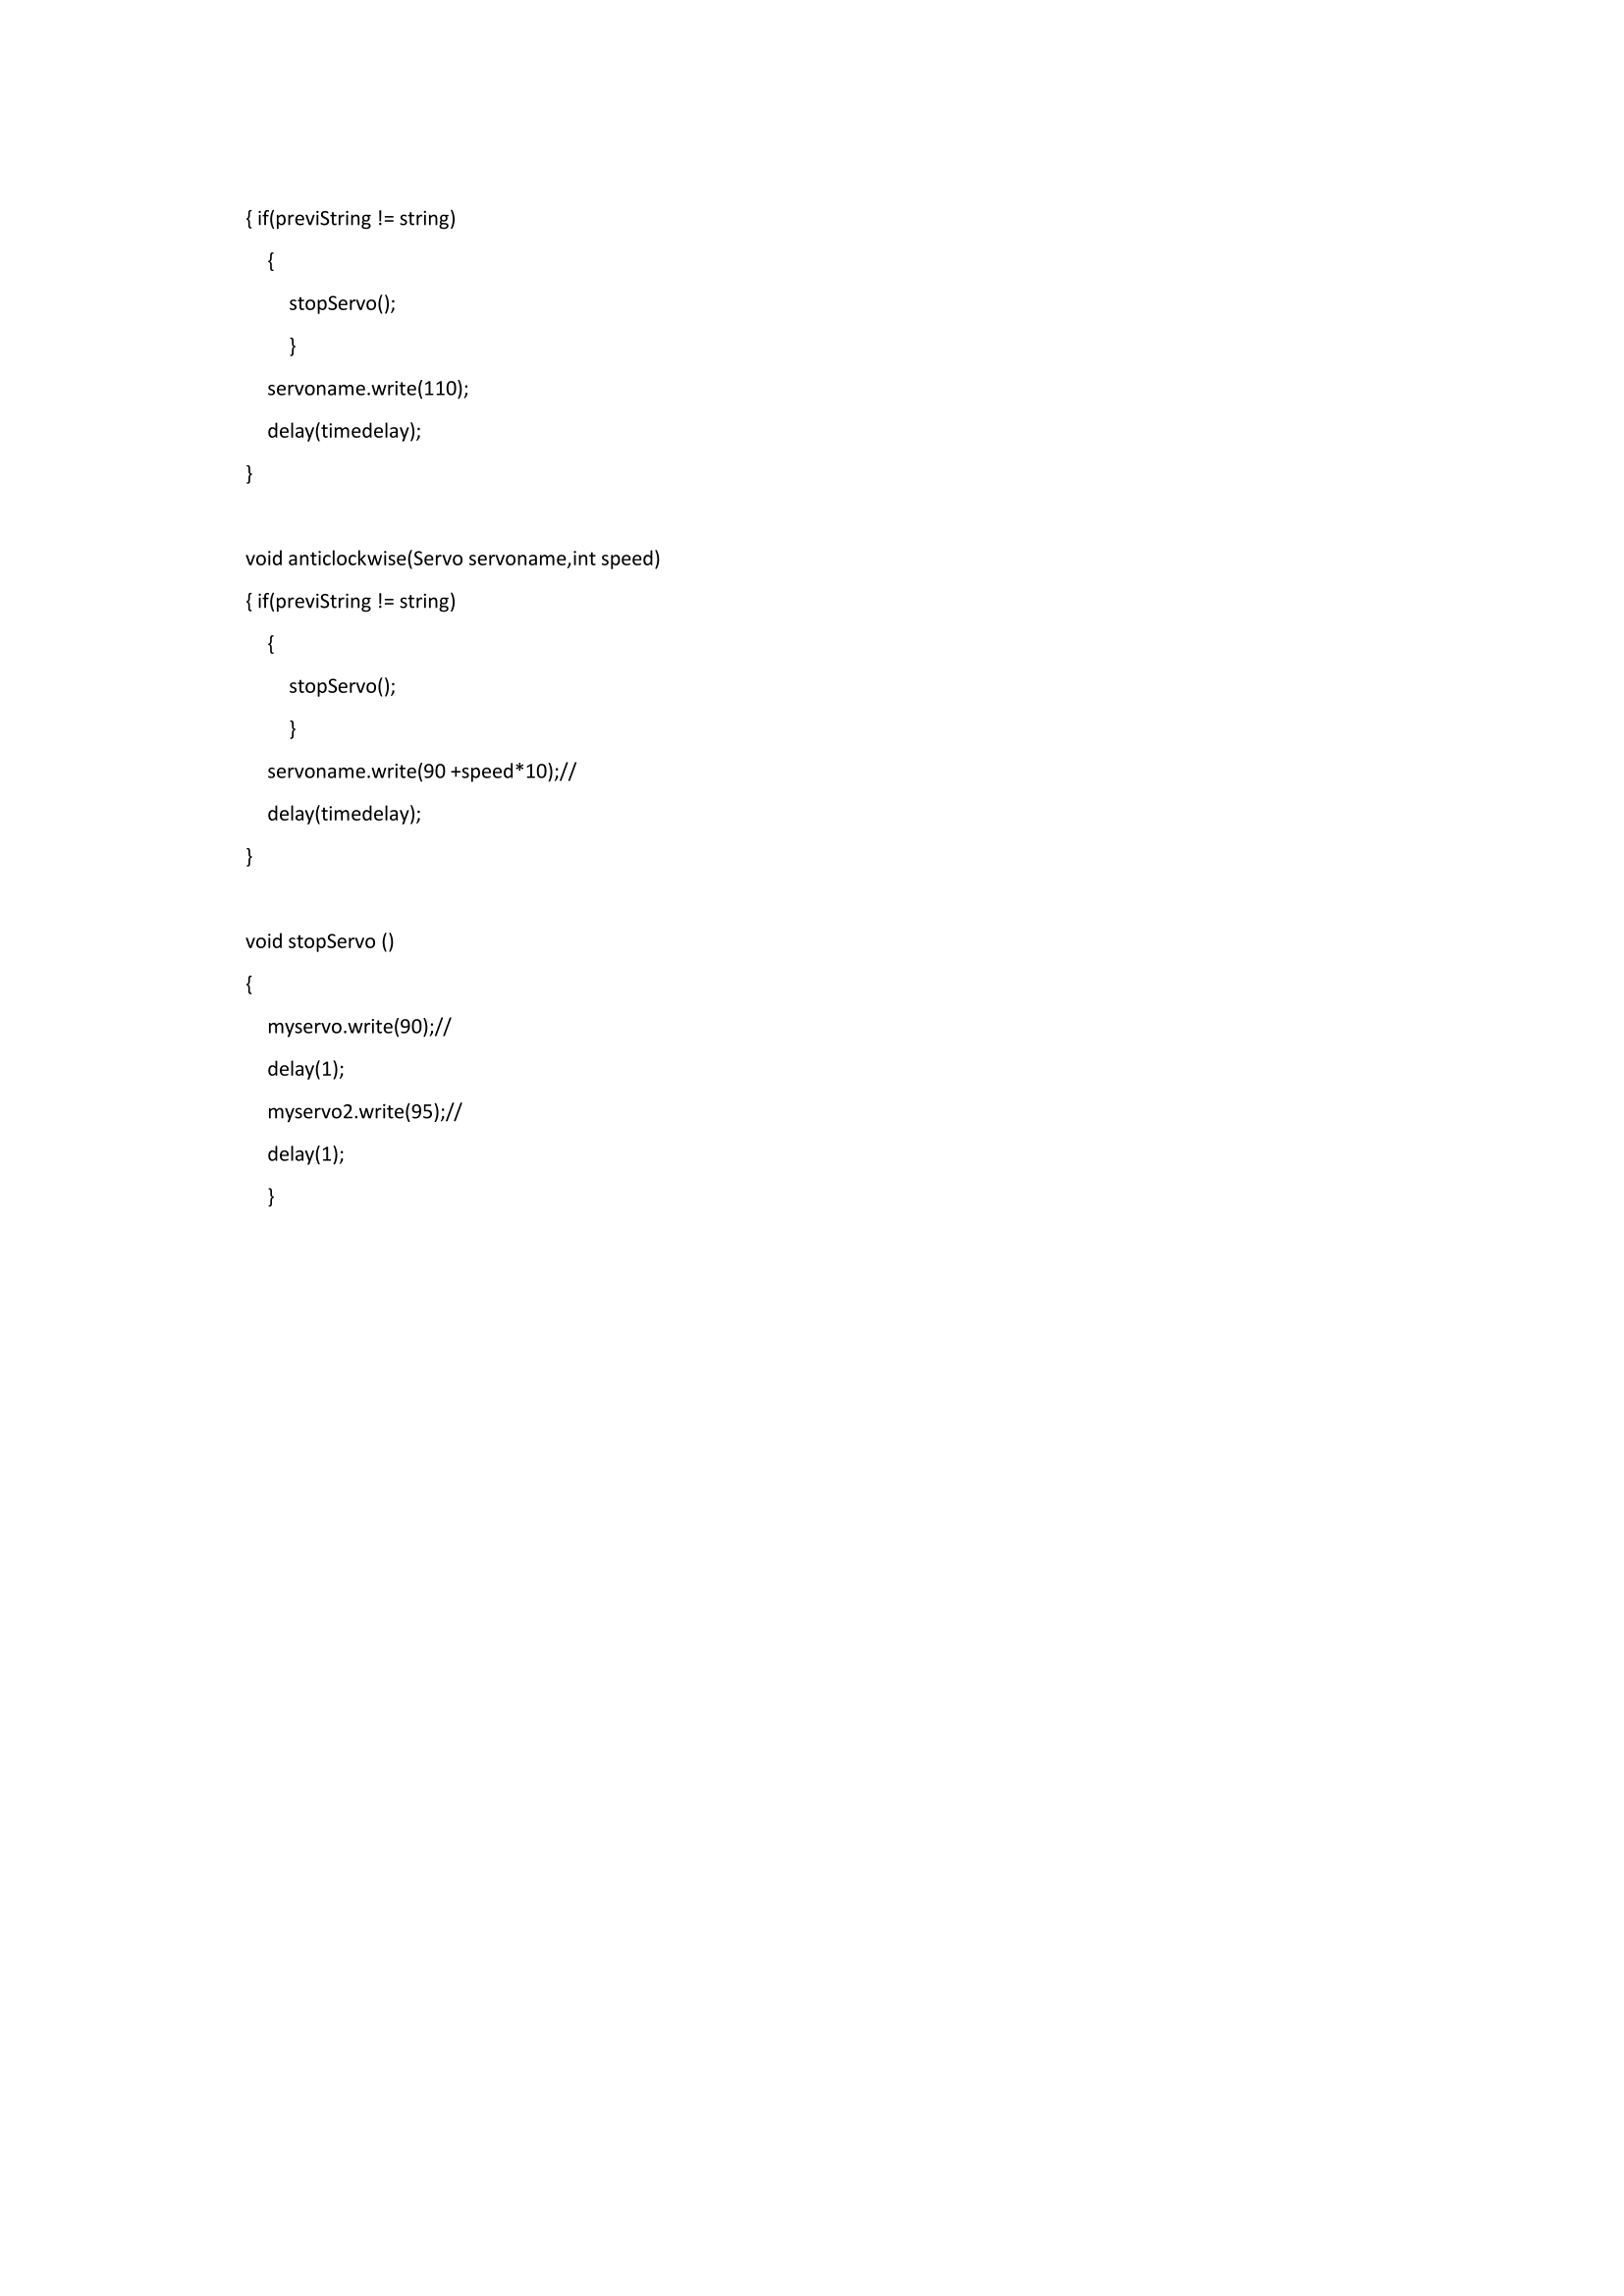
\includegraphics[width=1\textwidth,height=0.7\textheight]{A_thesis/appendix/code_arduino-2.png}
\end{figure}
\newpage

\section{Questionnaire of the Experiment1}
\begin{figure}[h]
\centering
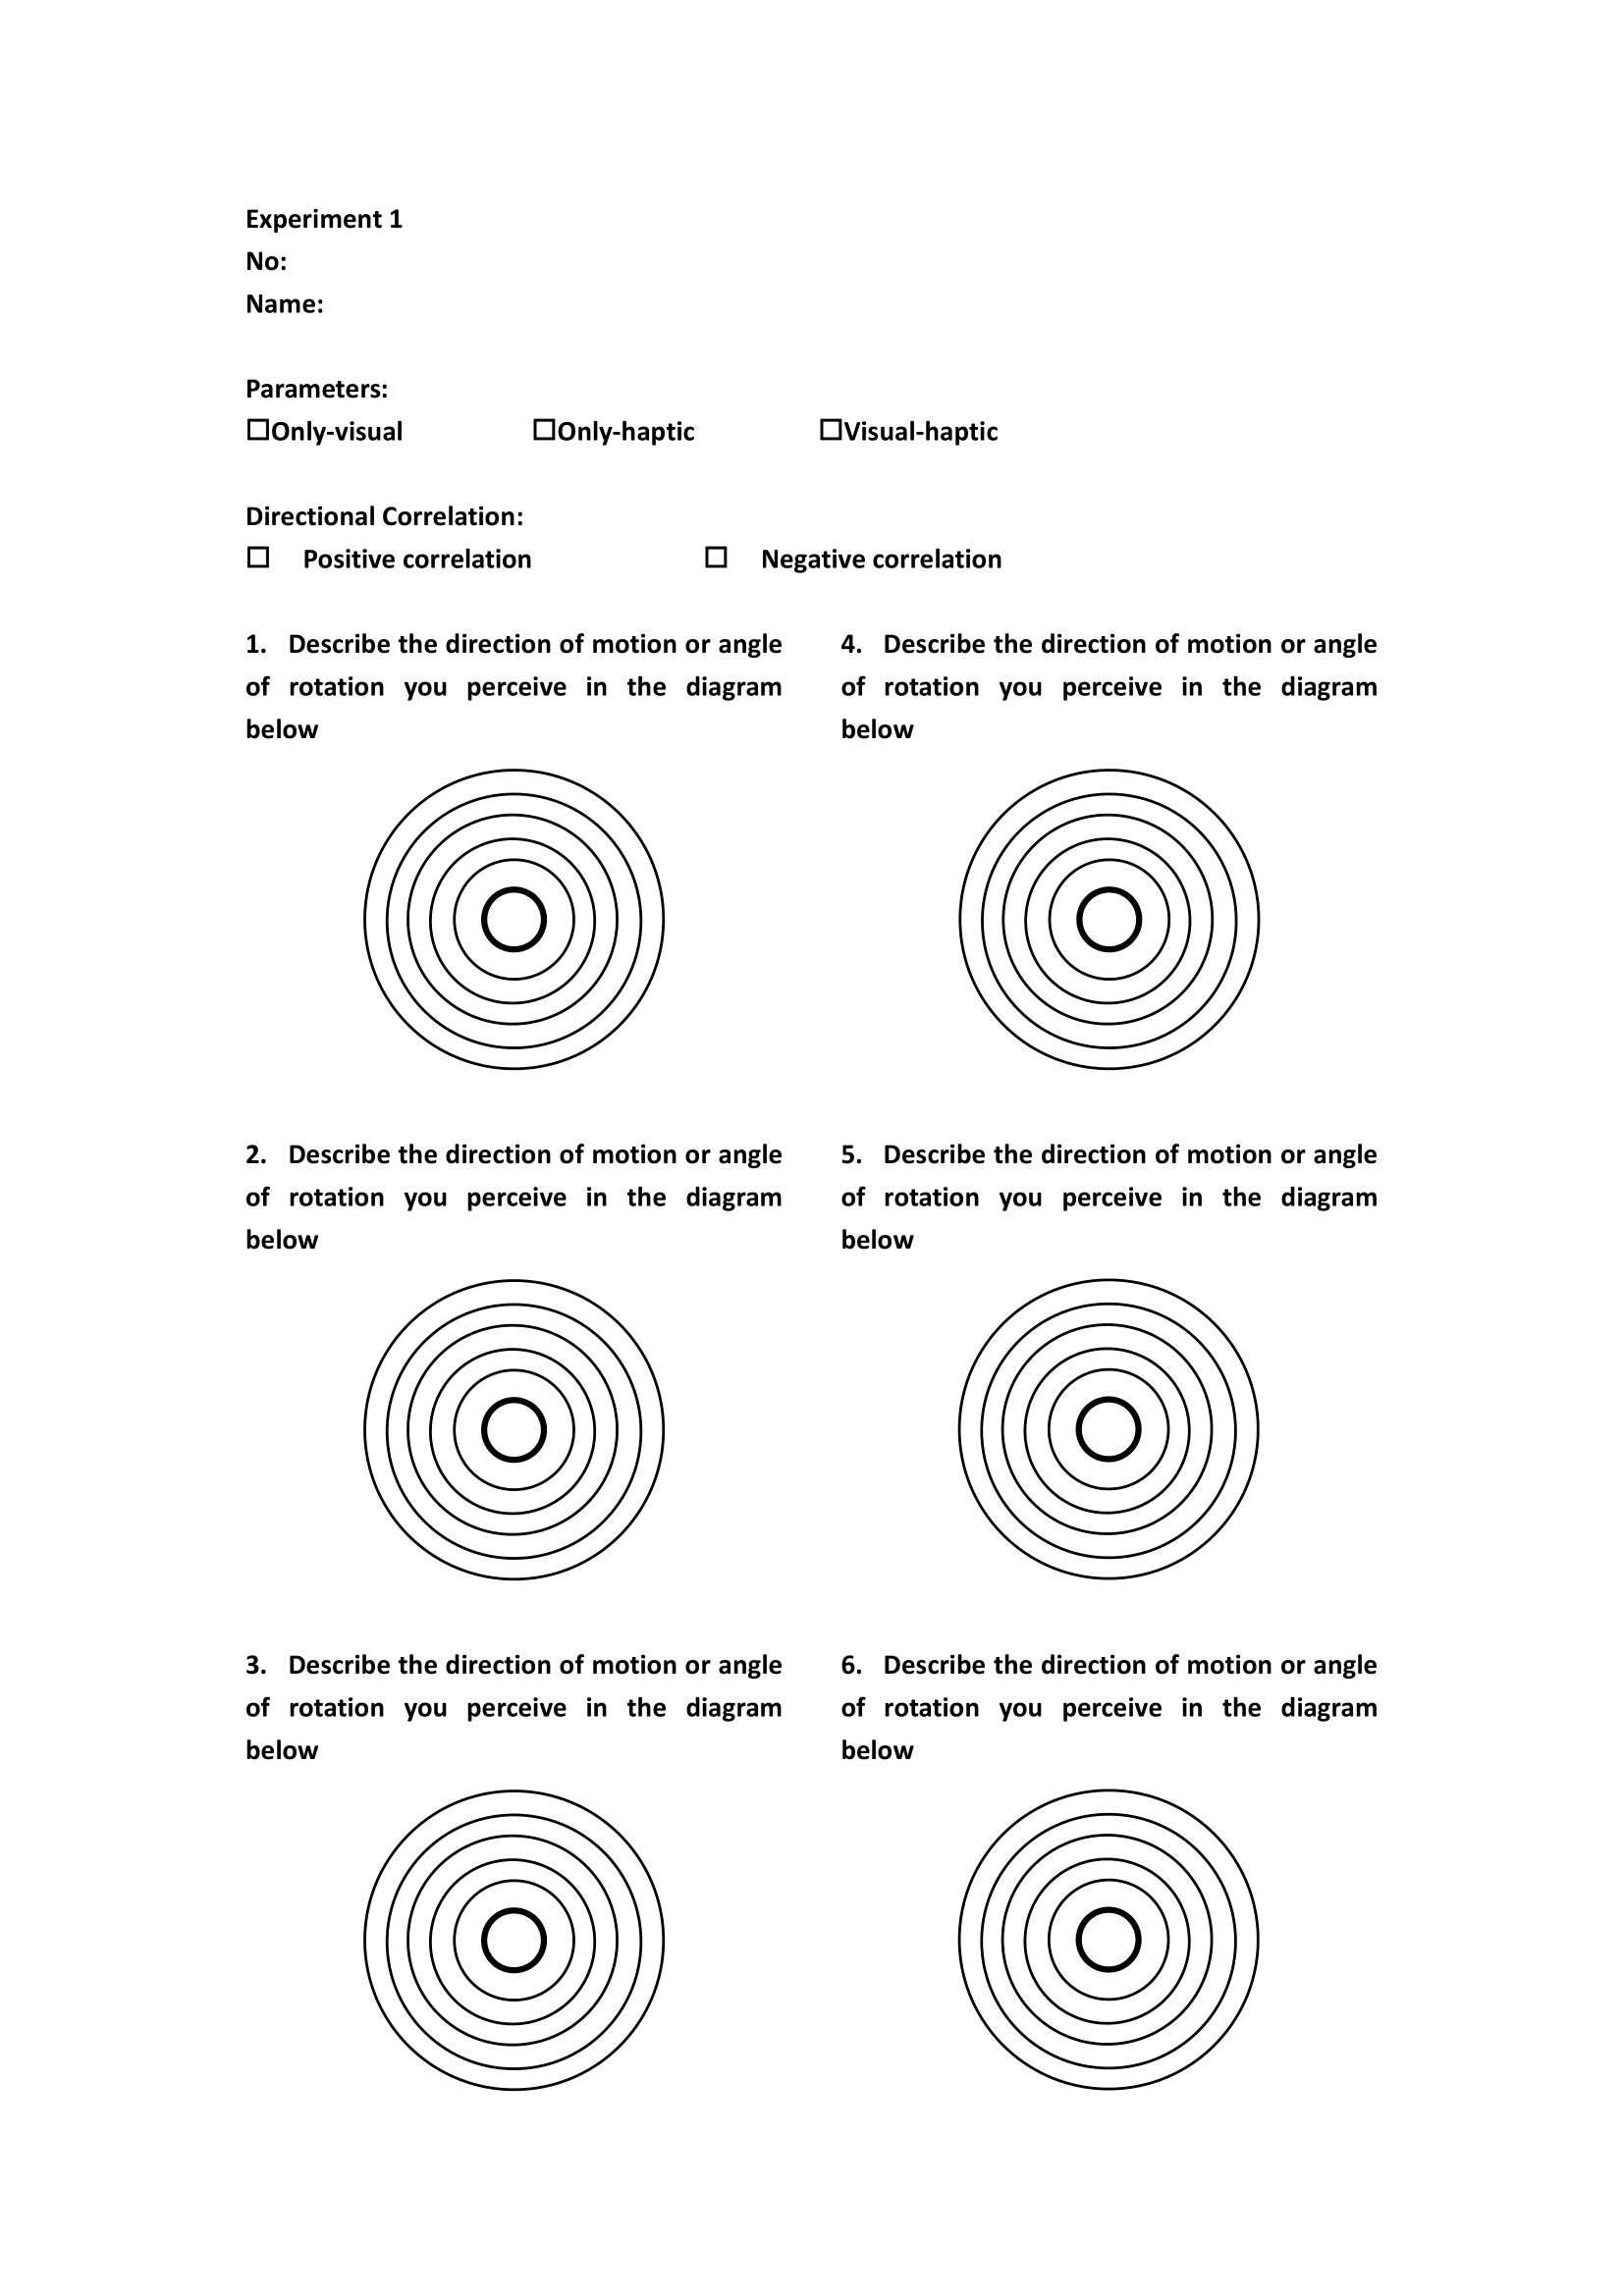
\includegraphics[width=1\textwidth,height=0.7\textheight]{A_thesis/appendix/Experiment1_questionnaire-1.png}
\end{figure}
\newpage

\begin{figure}[h]
\centering
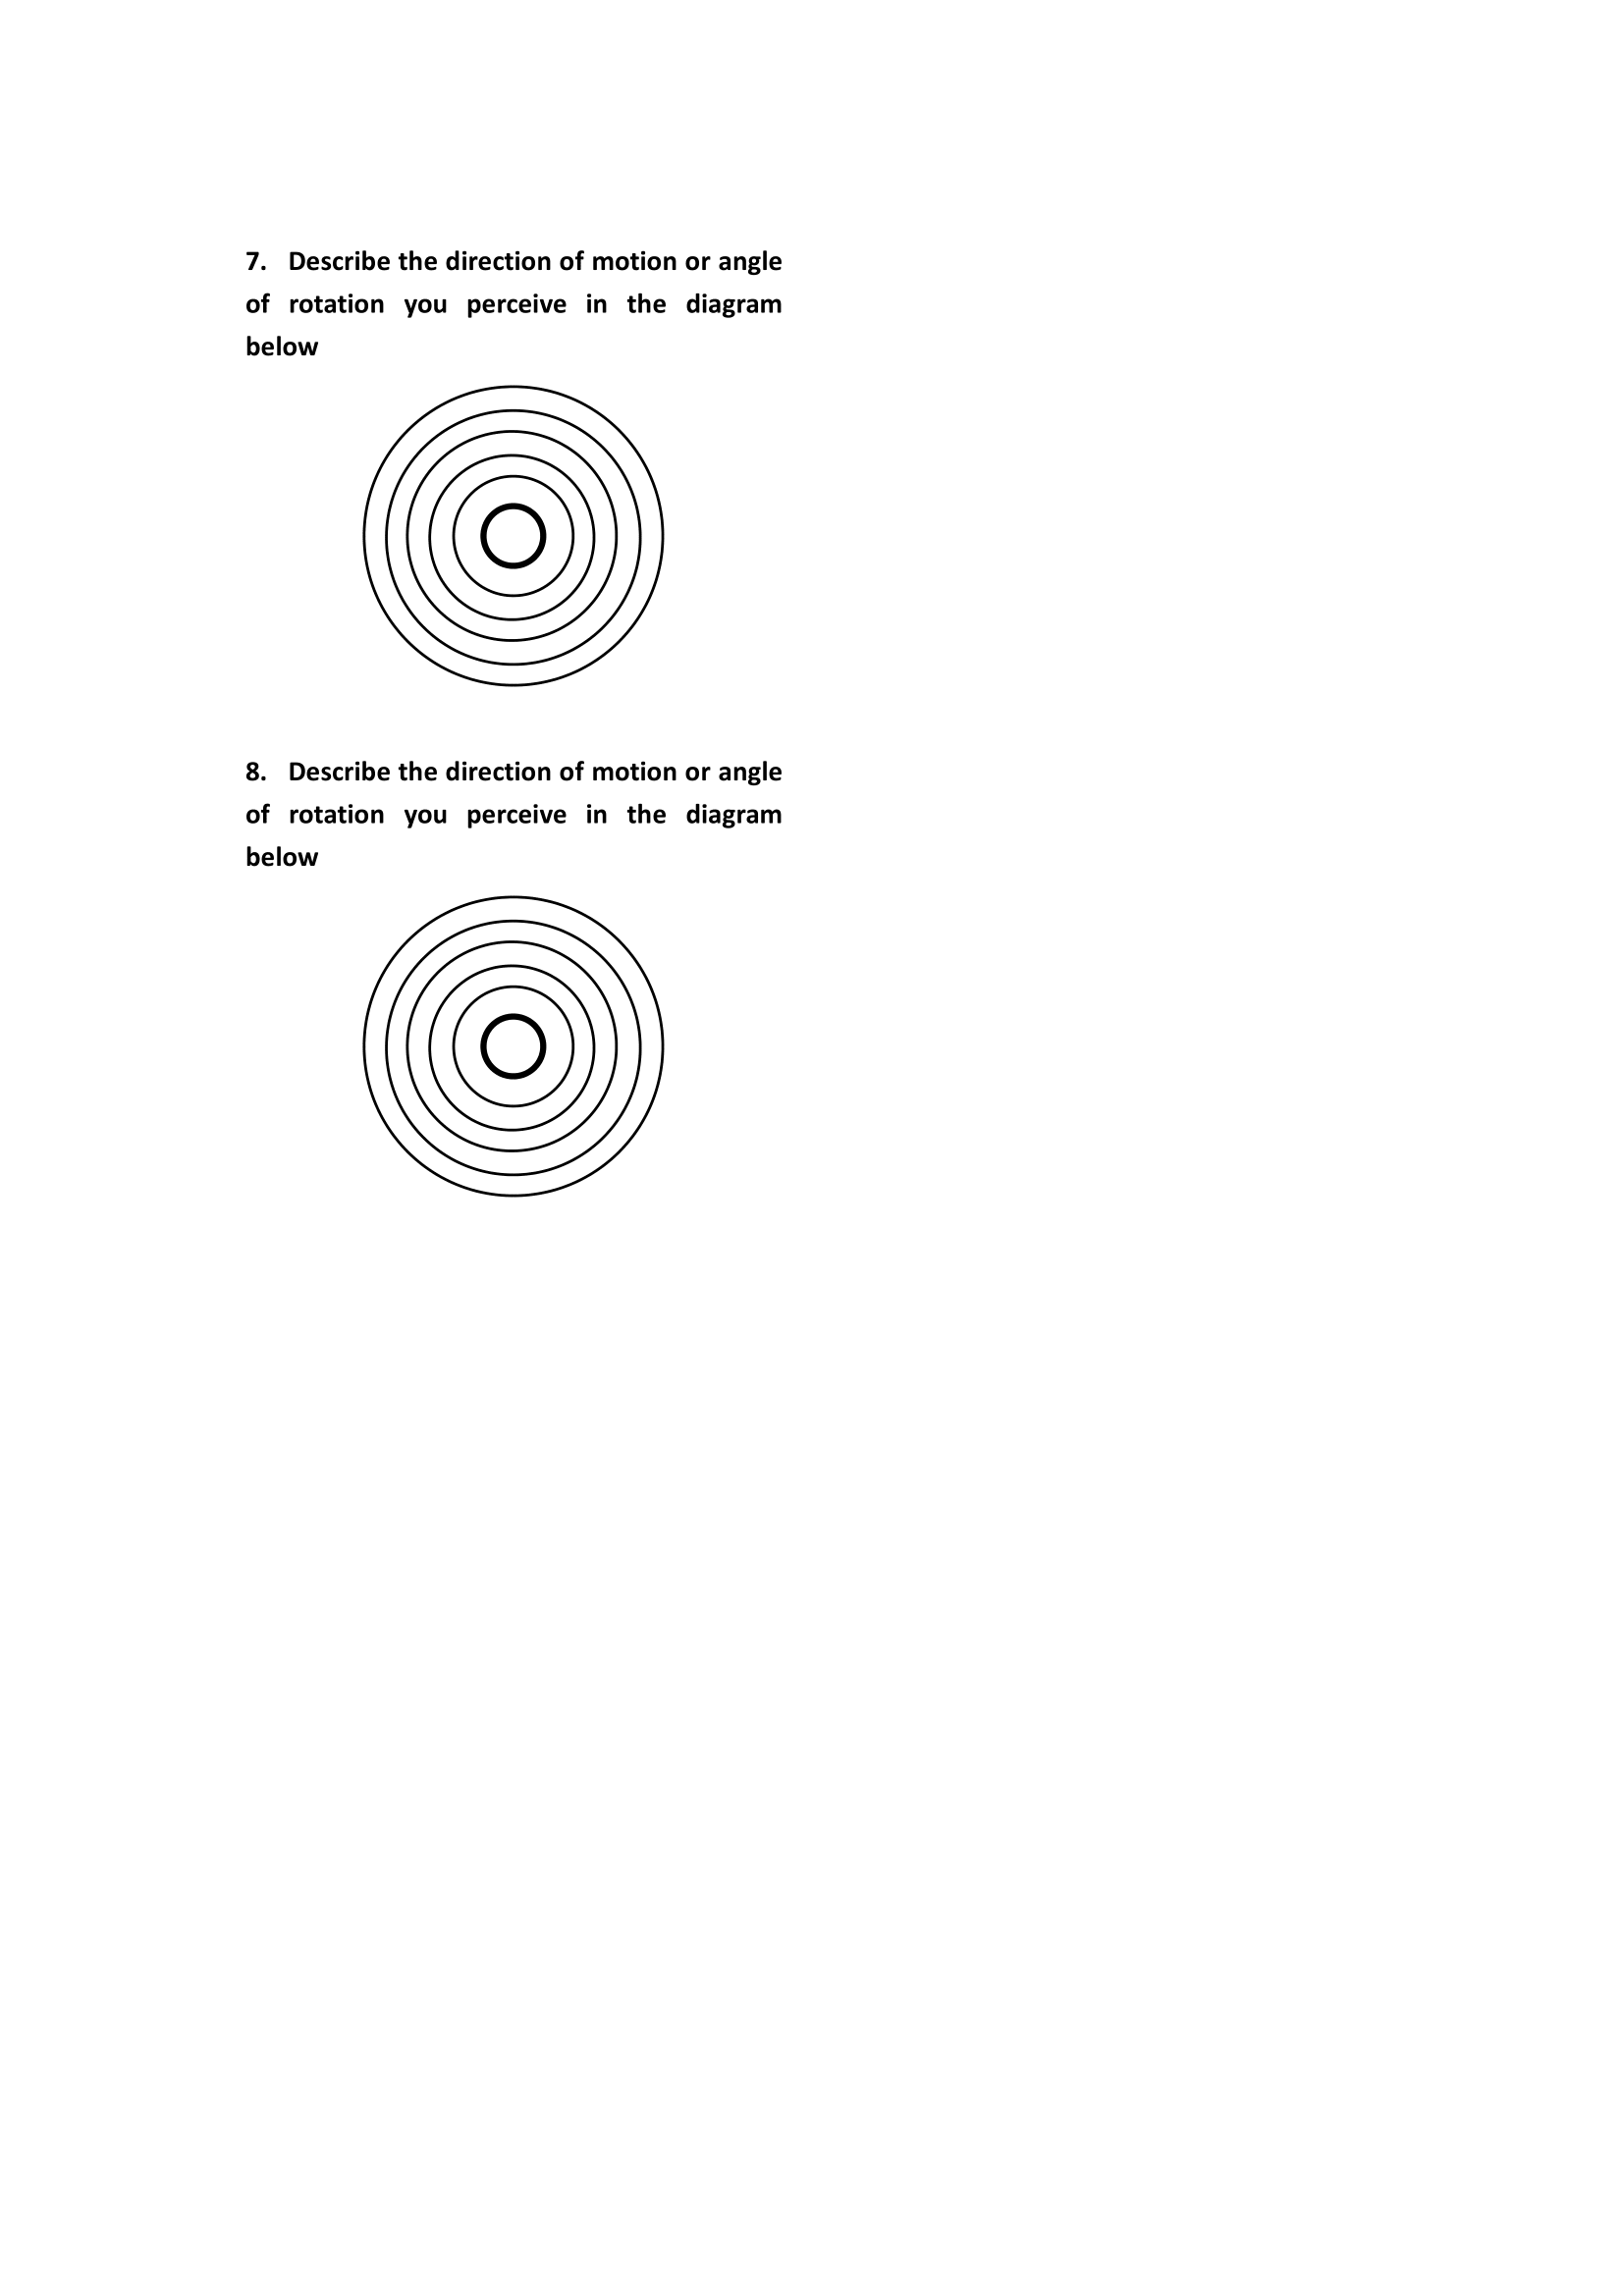
\includegraphics[width=1\textwidth,height=0.7\textheight]{A_thesis/appendix/Experiment1_questionnaire-2.png}
\end{figure}
\newpage

\begin{figure}[h]
\centering
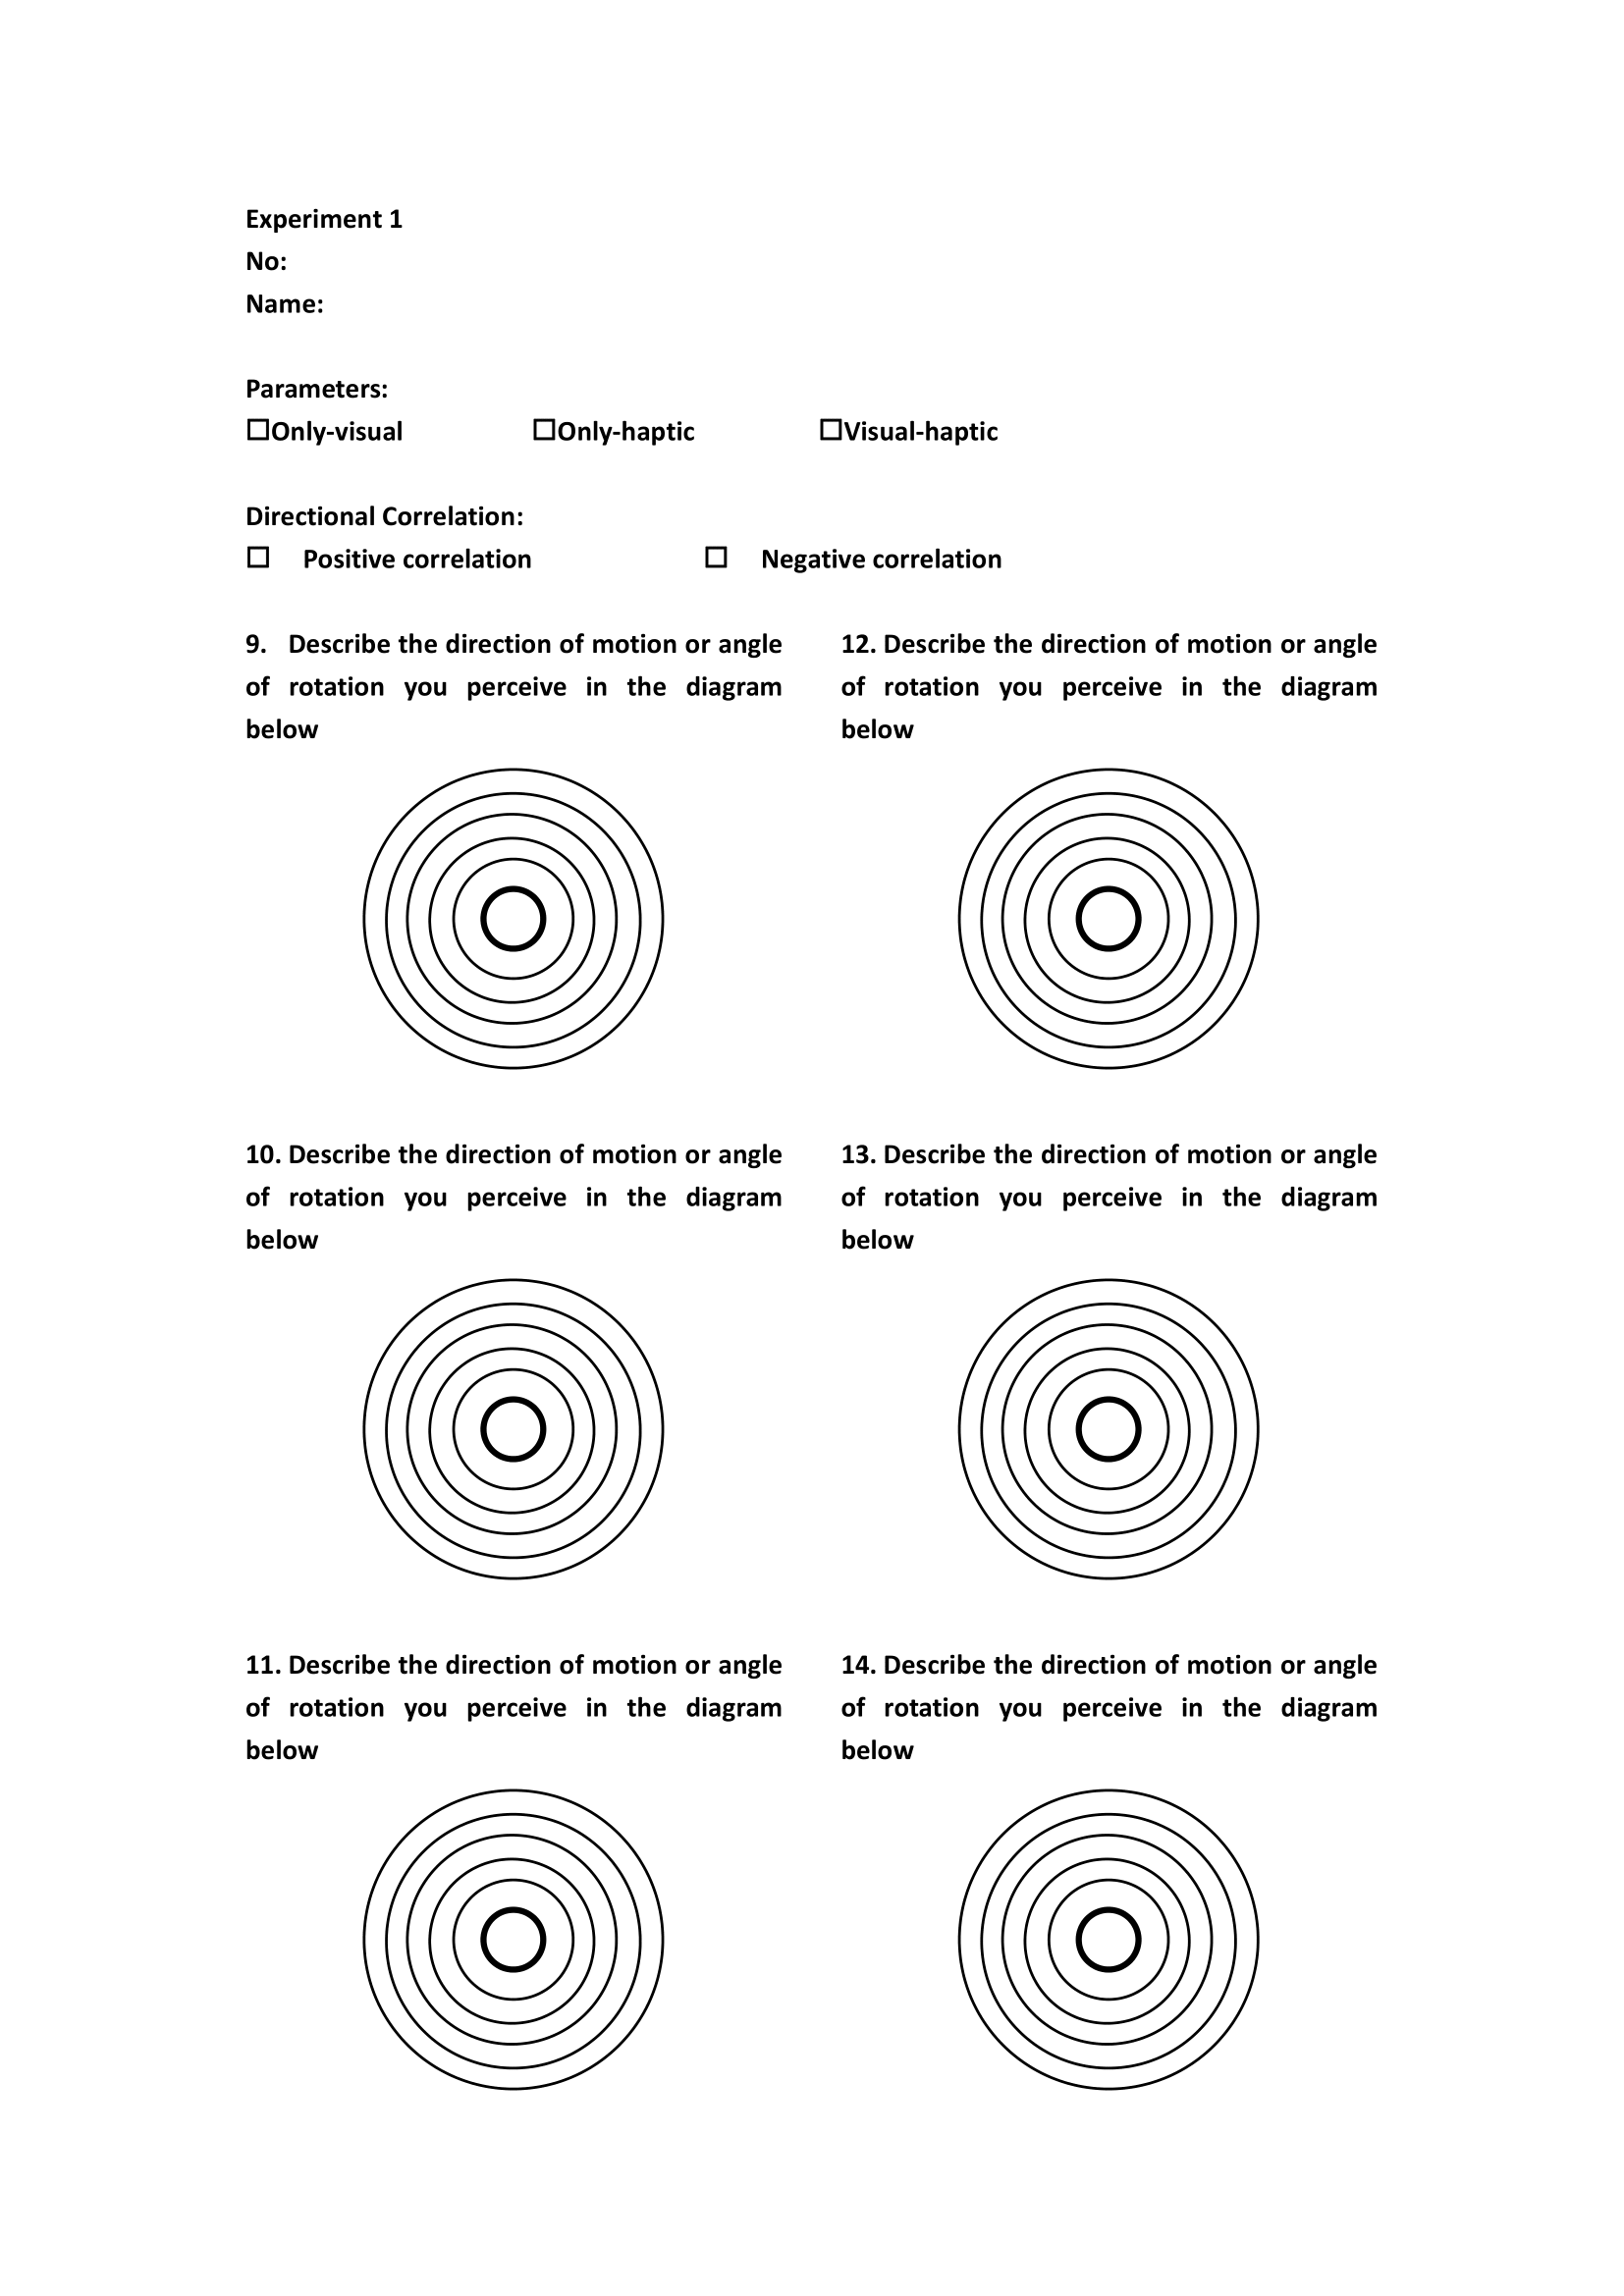
\includegraphics[width=1\textwidth,height=0.7\textheight]{A_thesis/appendix/Experiment1_questionnaire-3.png}
\end{figure}
\newpage

\begin{figure}[h]
\centering
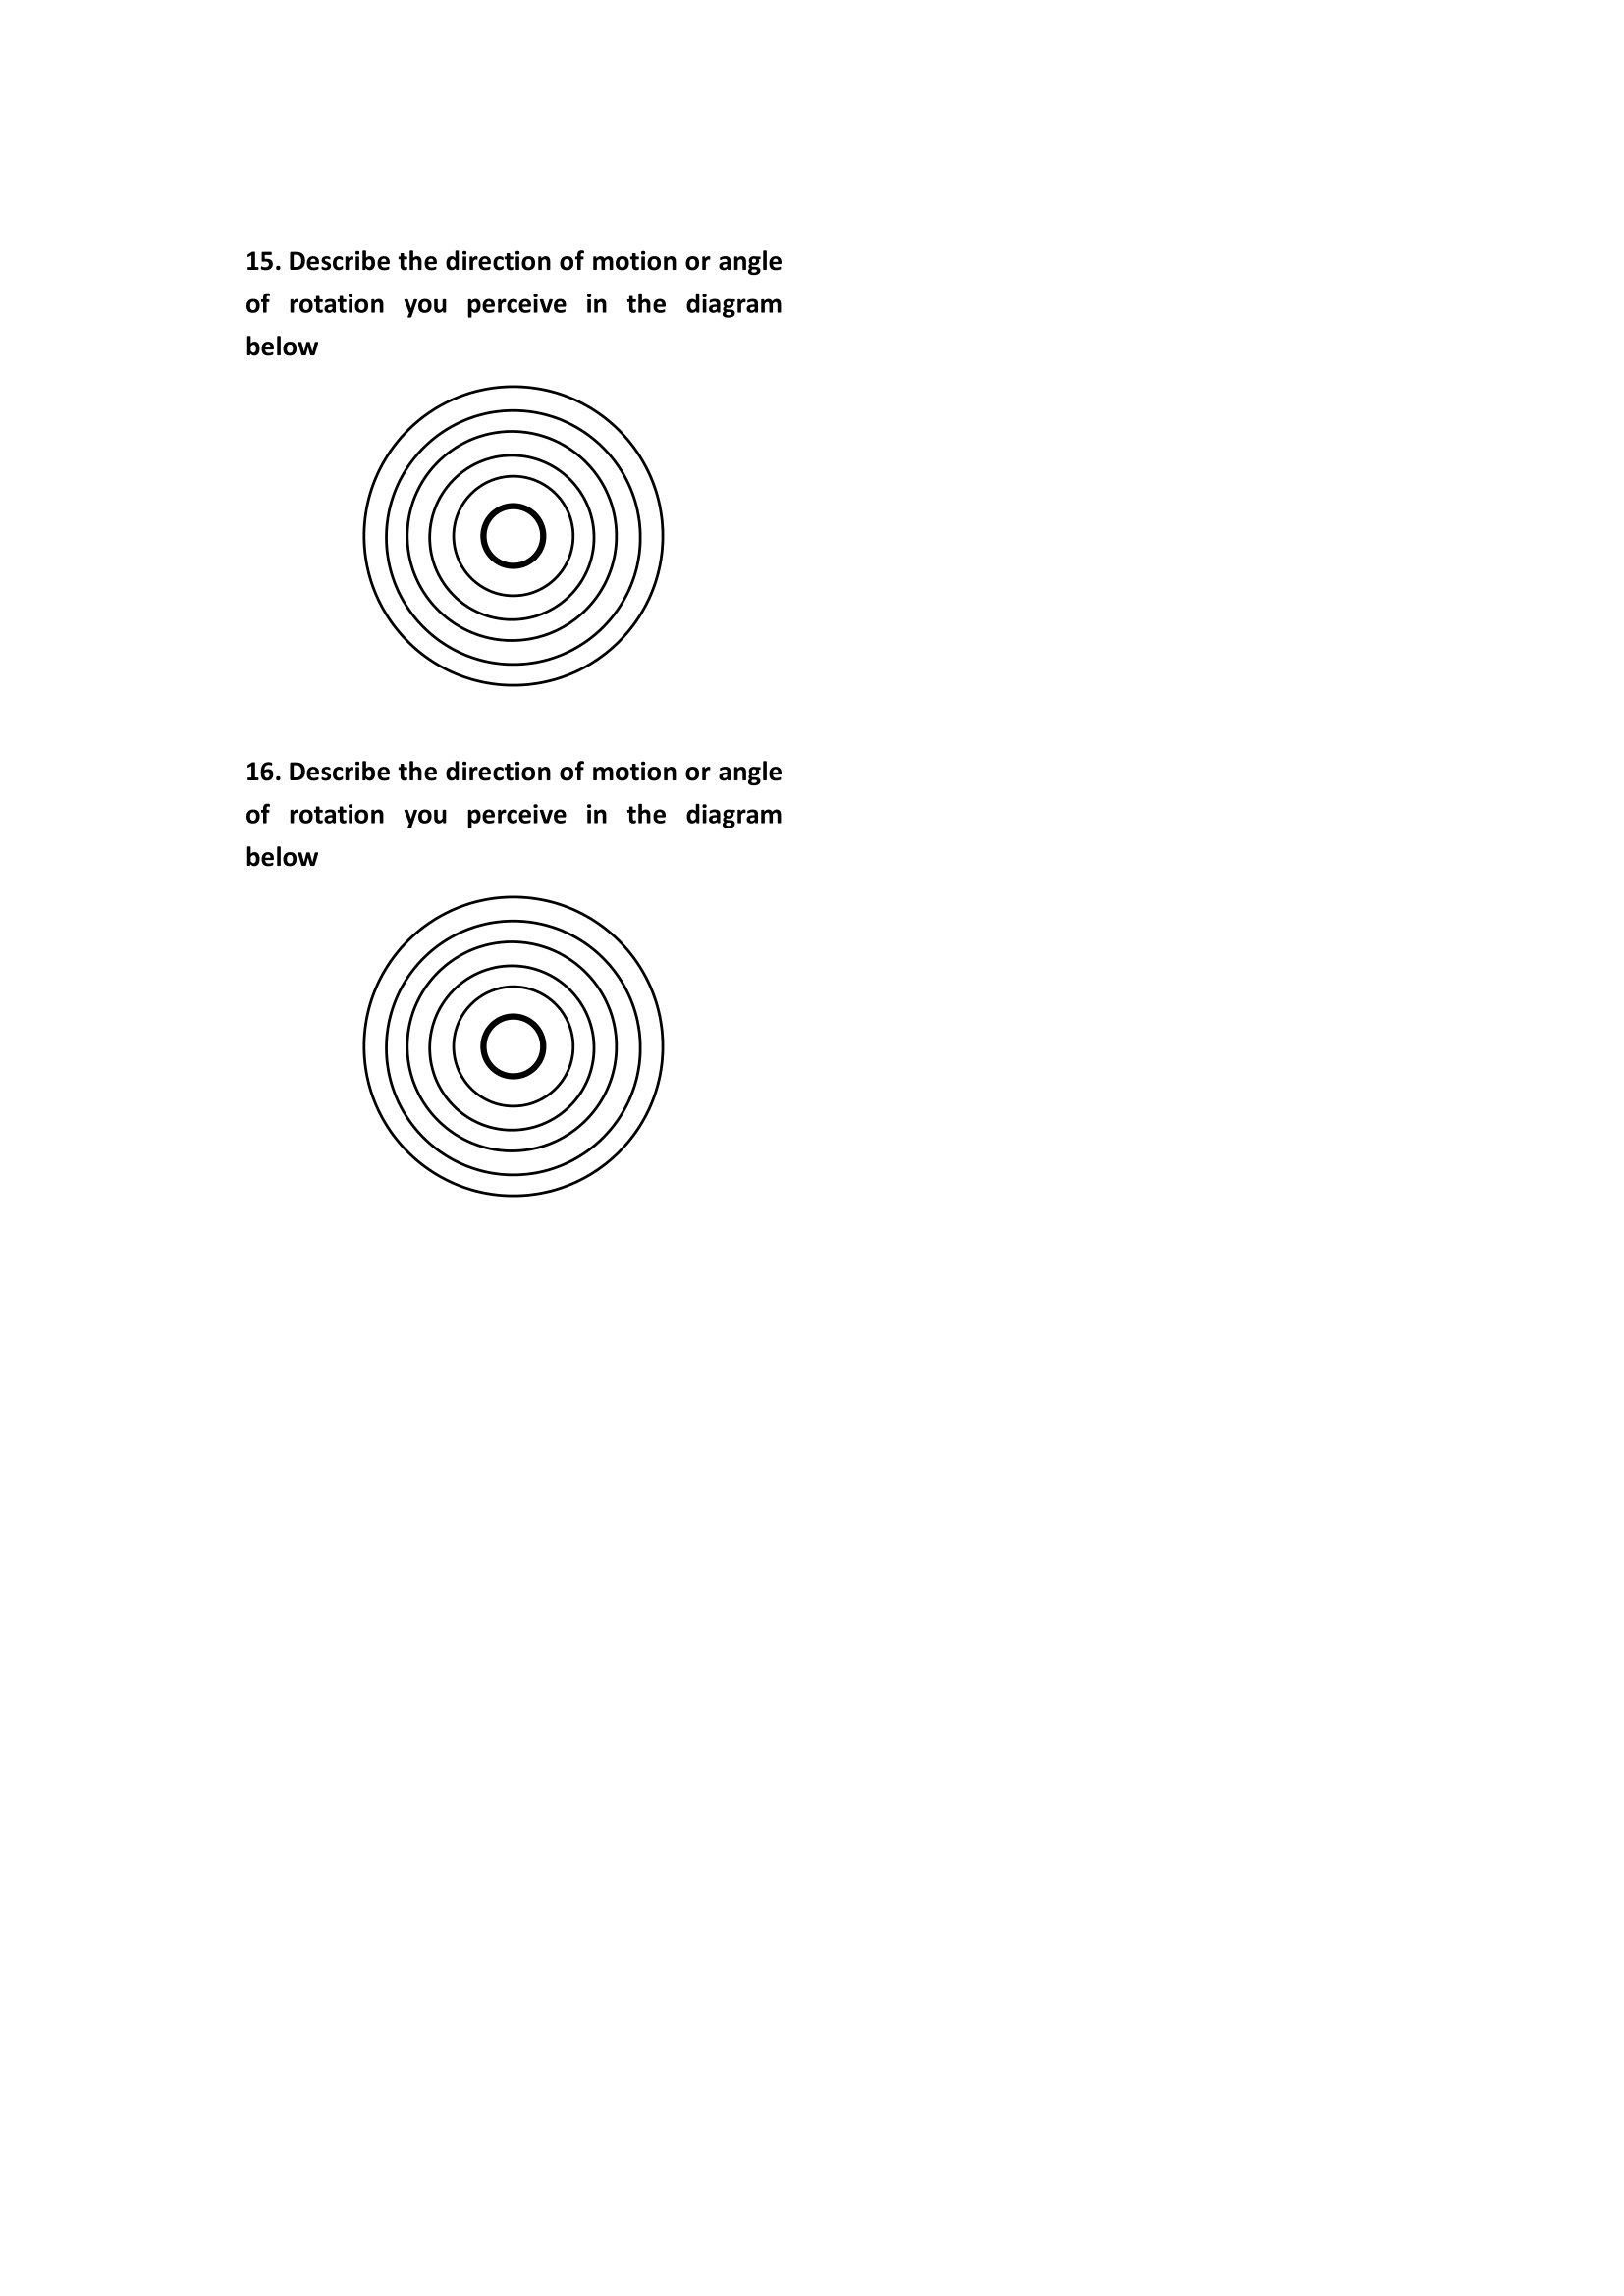
\includegraphics[width=1\textwidth,height=0.7\textheight]{A_thesis/appendix/Experiment1_questionnaire-4.png}
\end{figure}
\newpage

\begin{figure}[h]
\centering
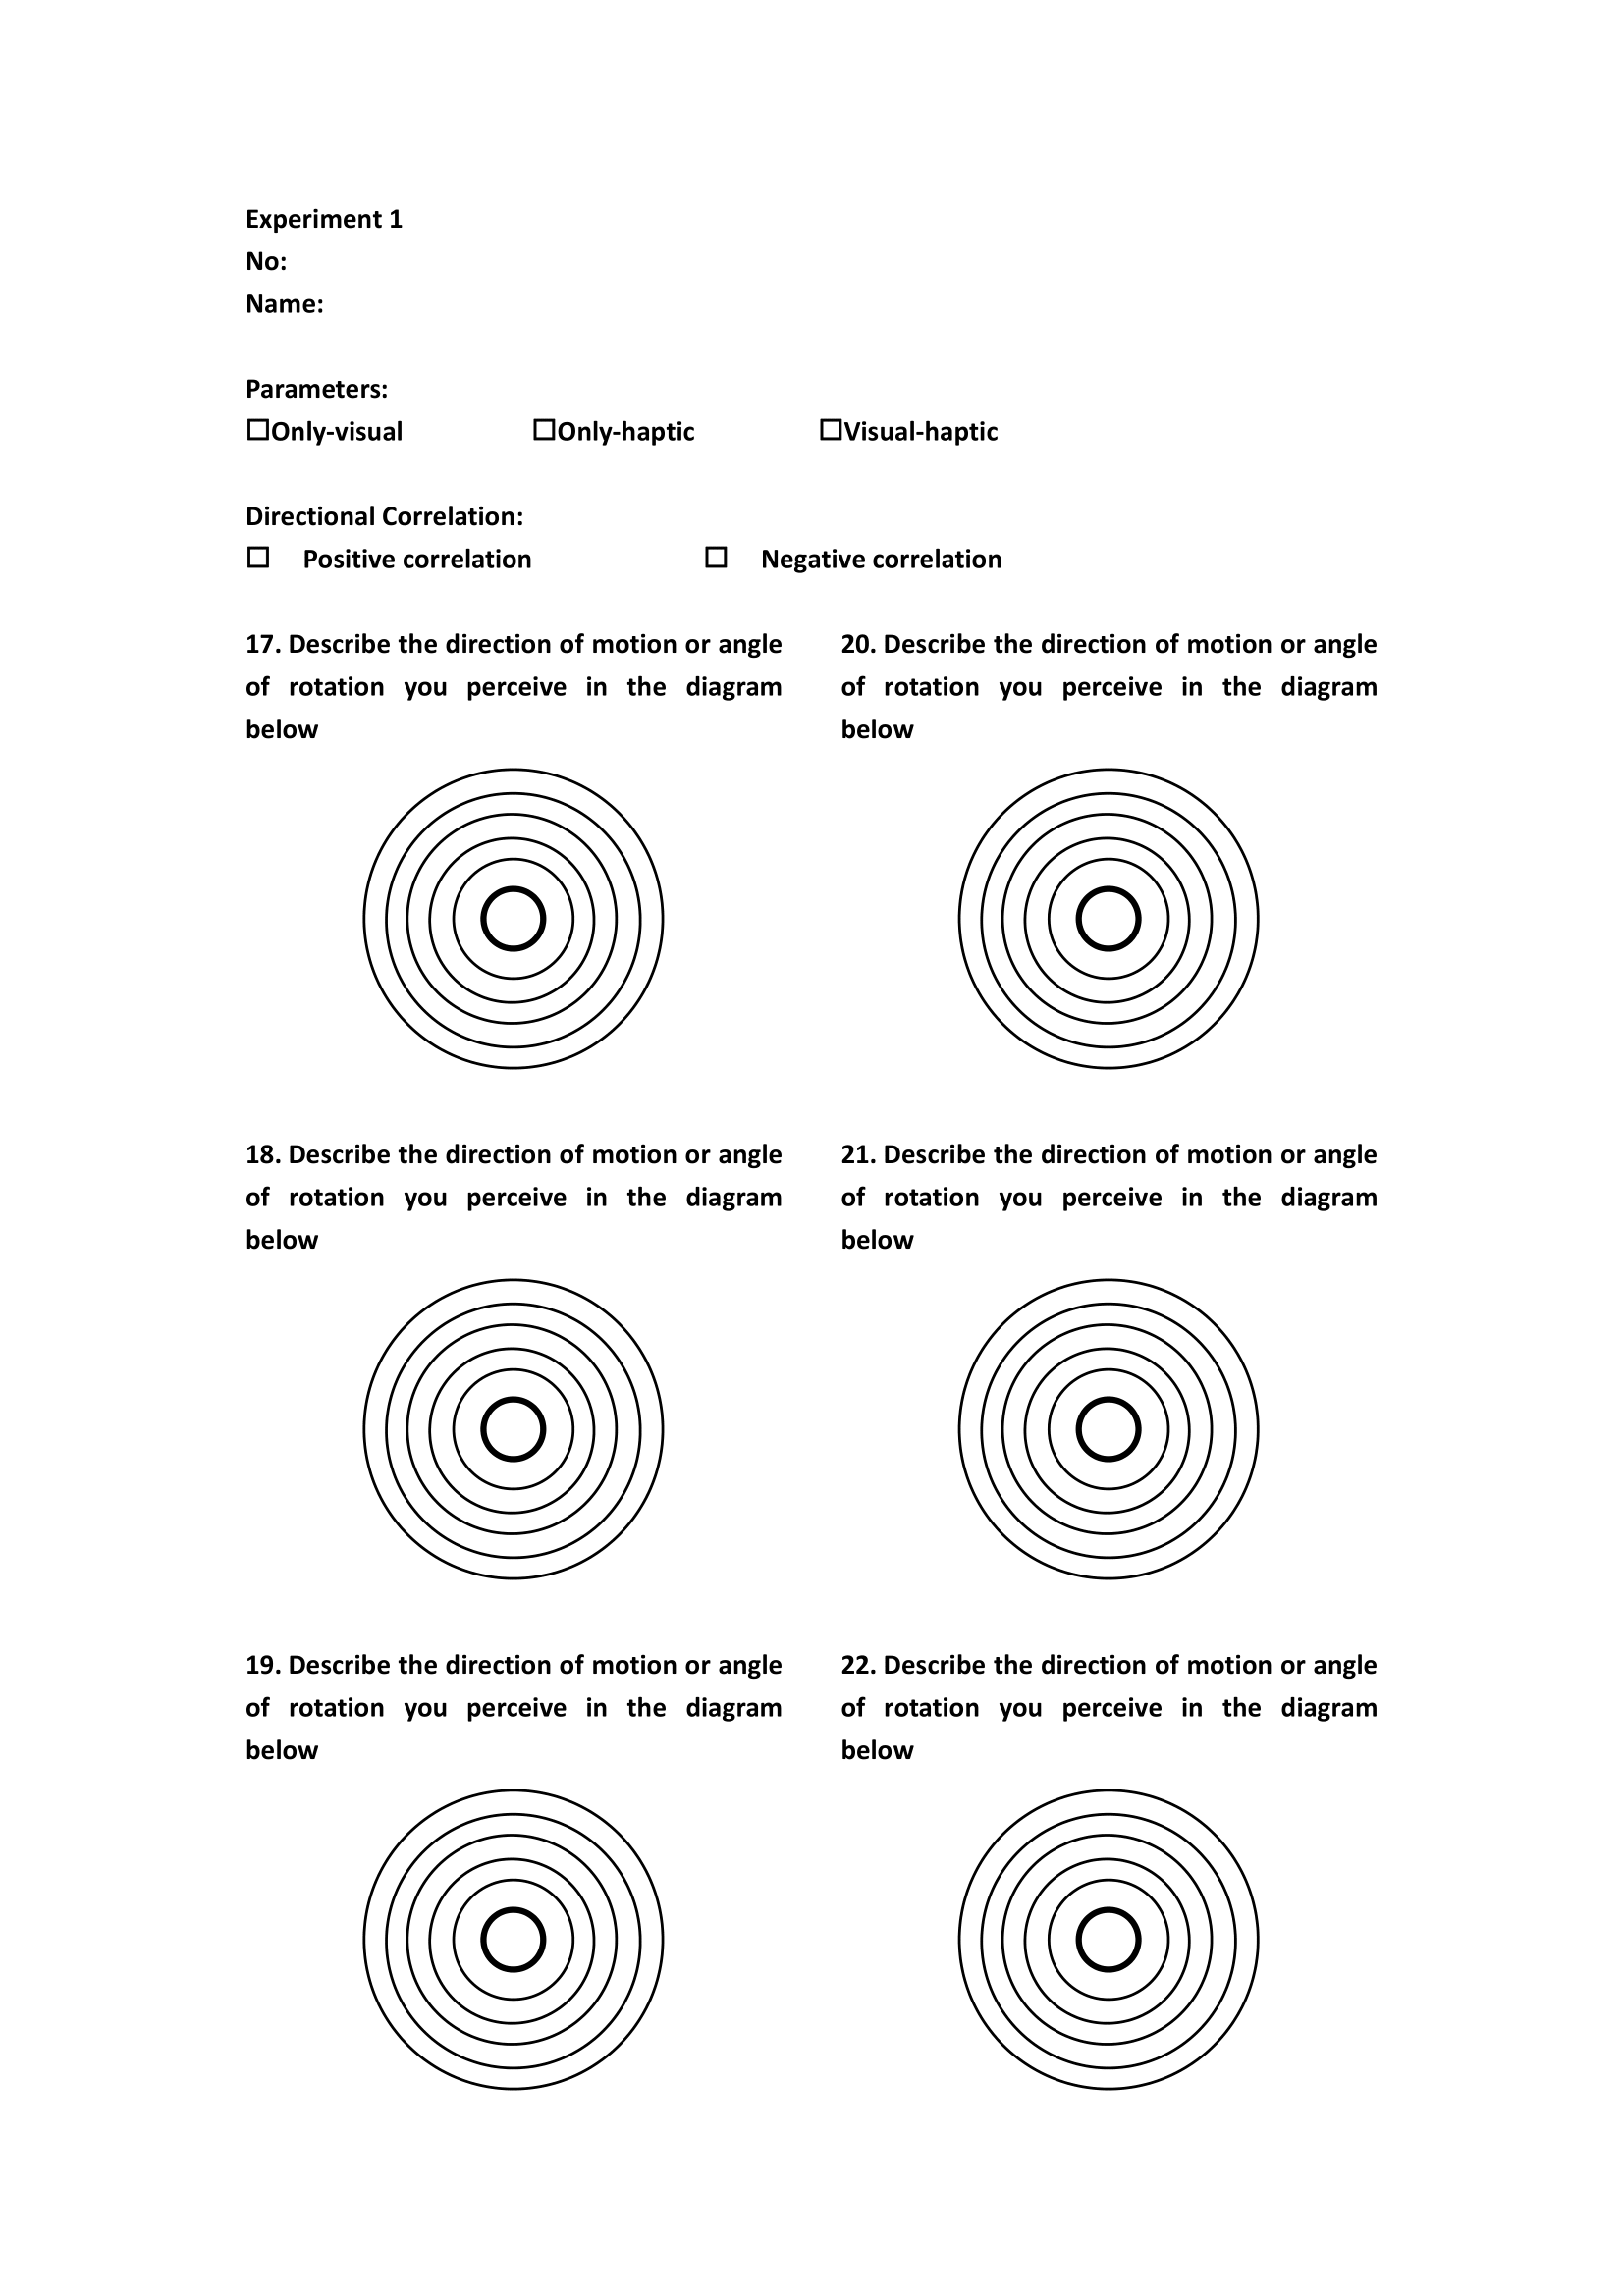
\includegraphics[width=1\textwidth,height=0.7\textheight]{A_thesis/appendix/Experiment1_questionnaire-5.png}
\end{figure}
\newpage

\begin{figure}[h]
\centering
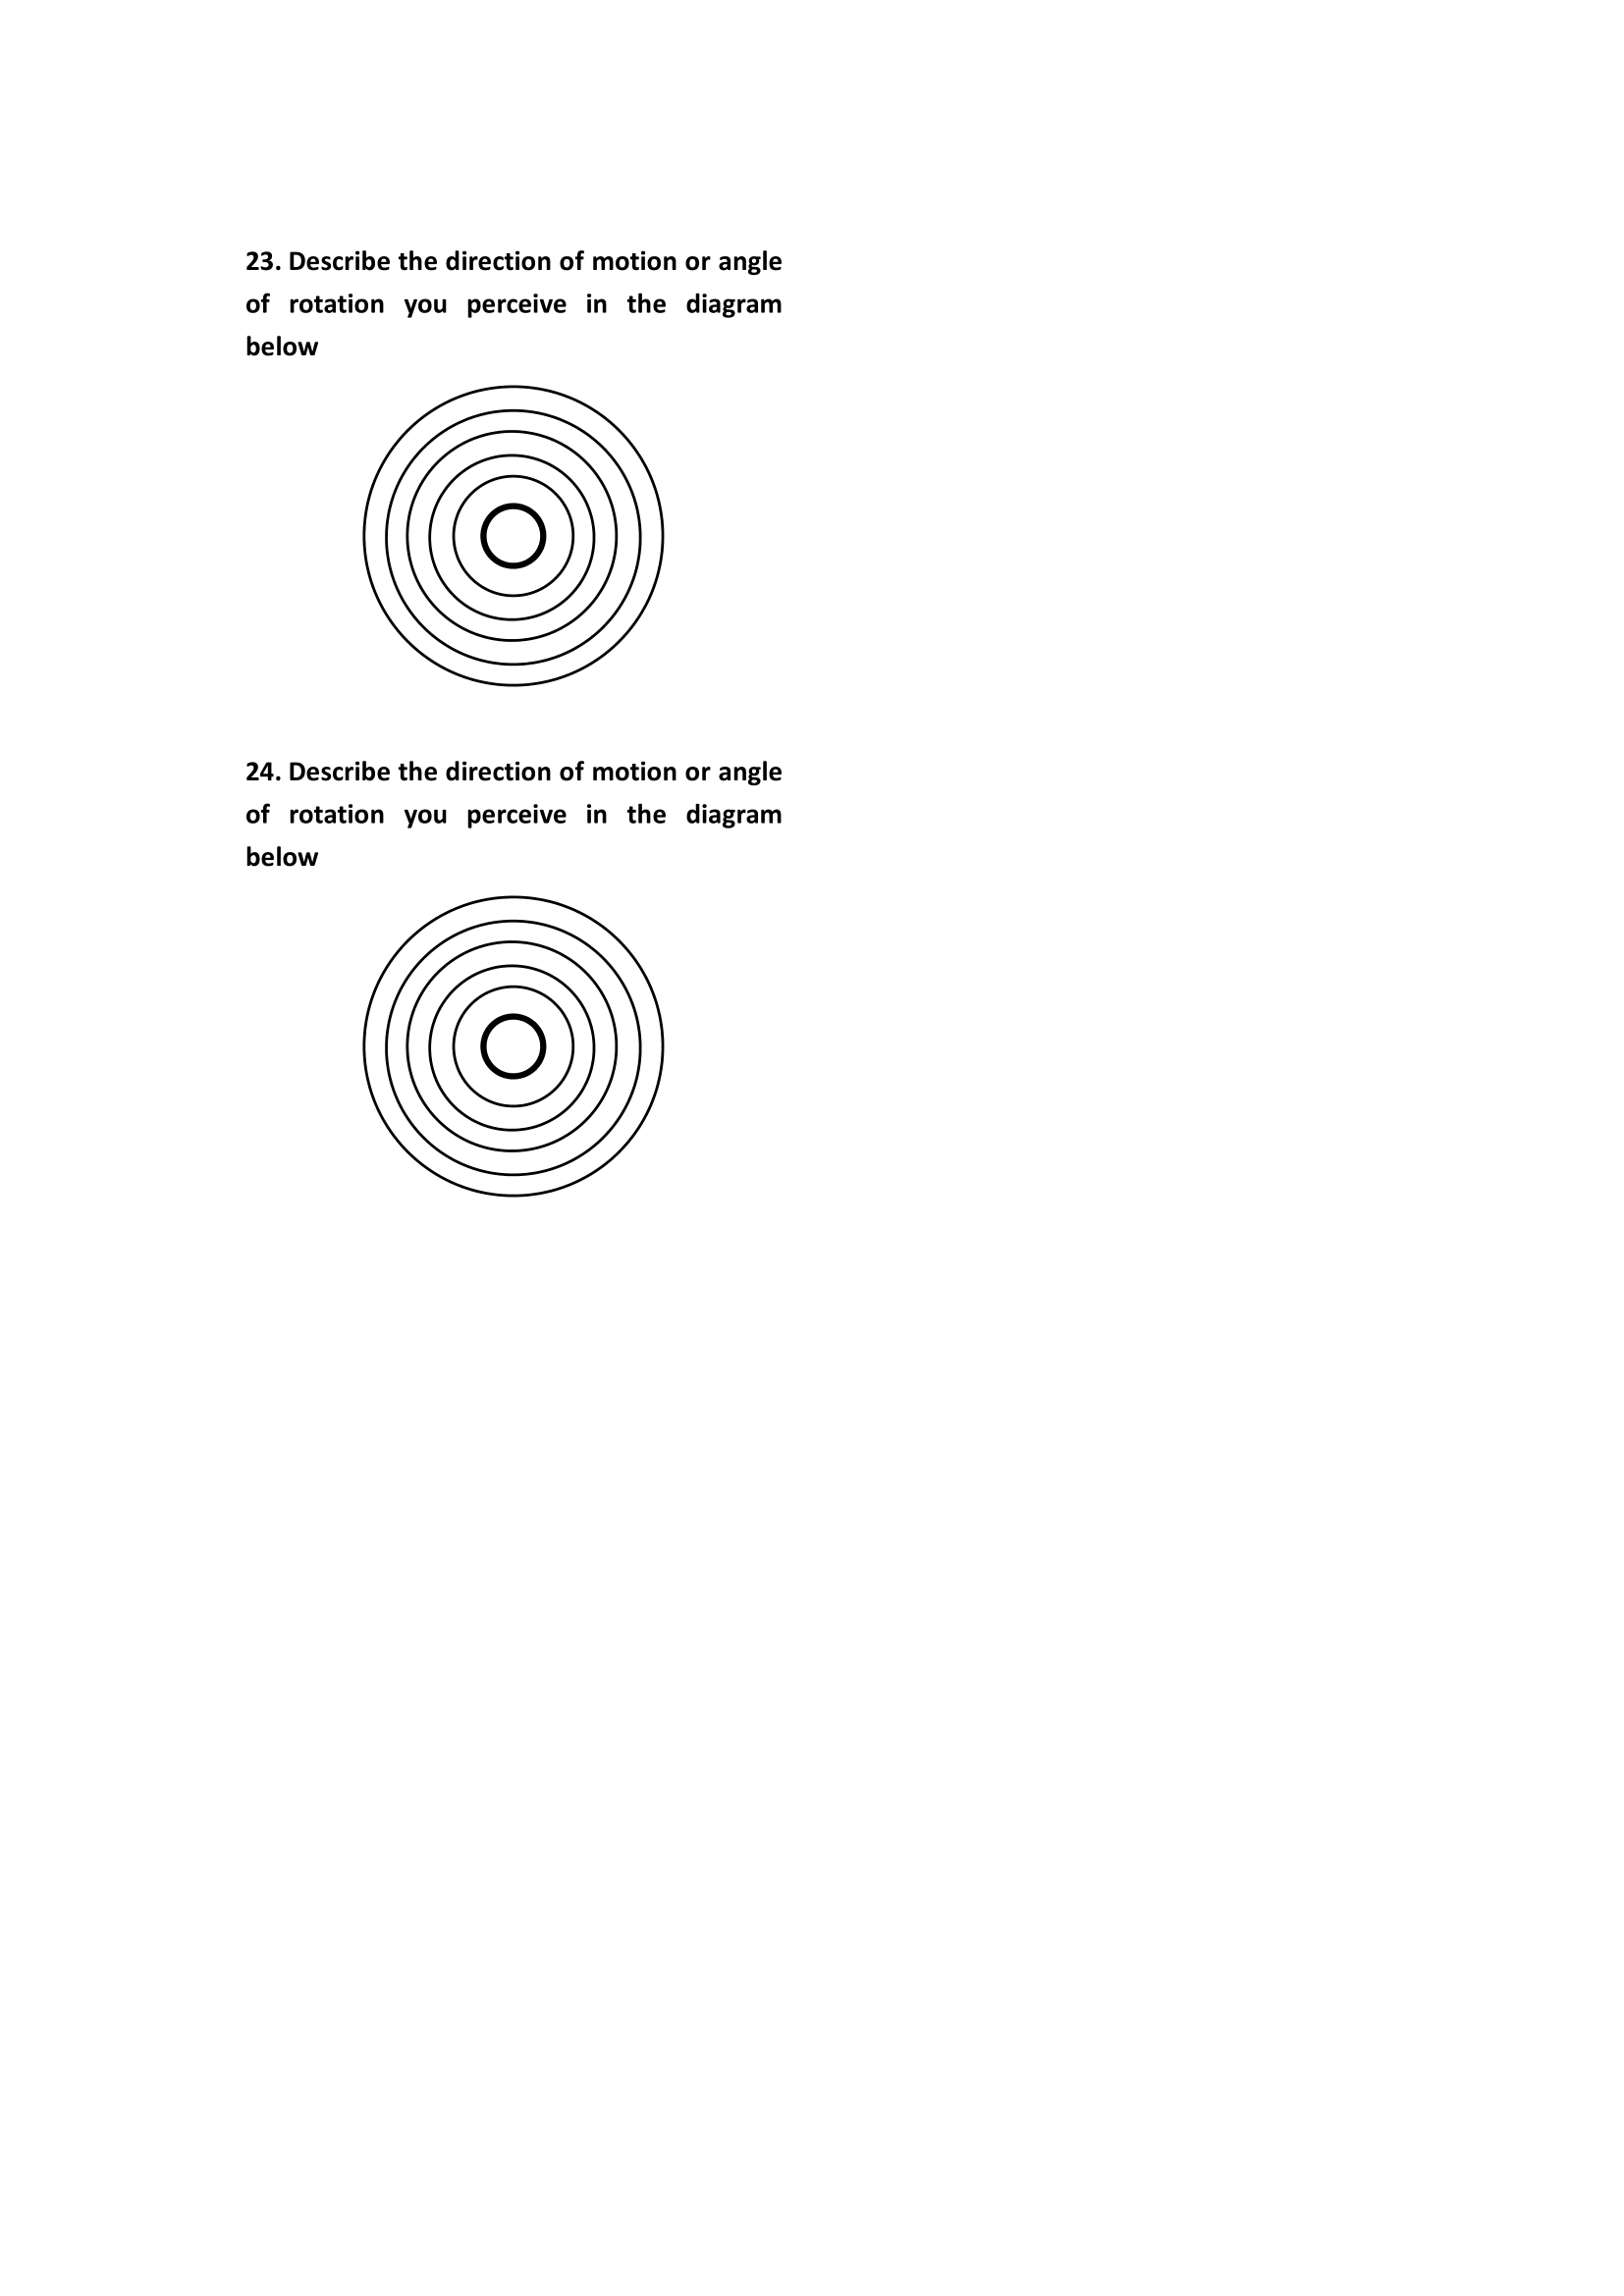
\includegraphics[width=1\textwidth,height=0.7\textheight]{A_thesis/appendix/Experiment1_questionnaire-6.png}
\end{figure}
\newpage

\begin{figure}[h]
\centering
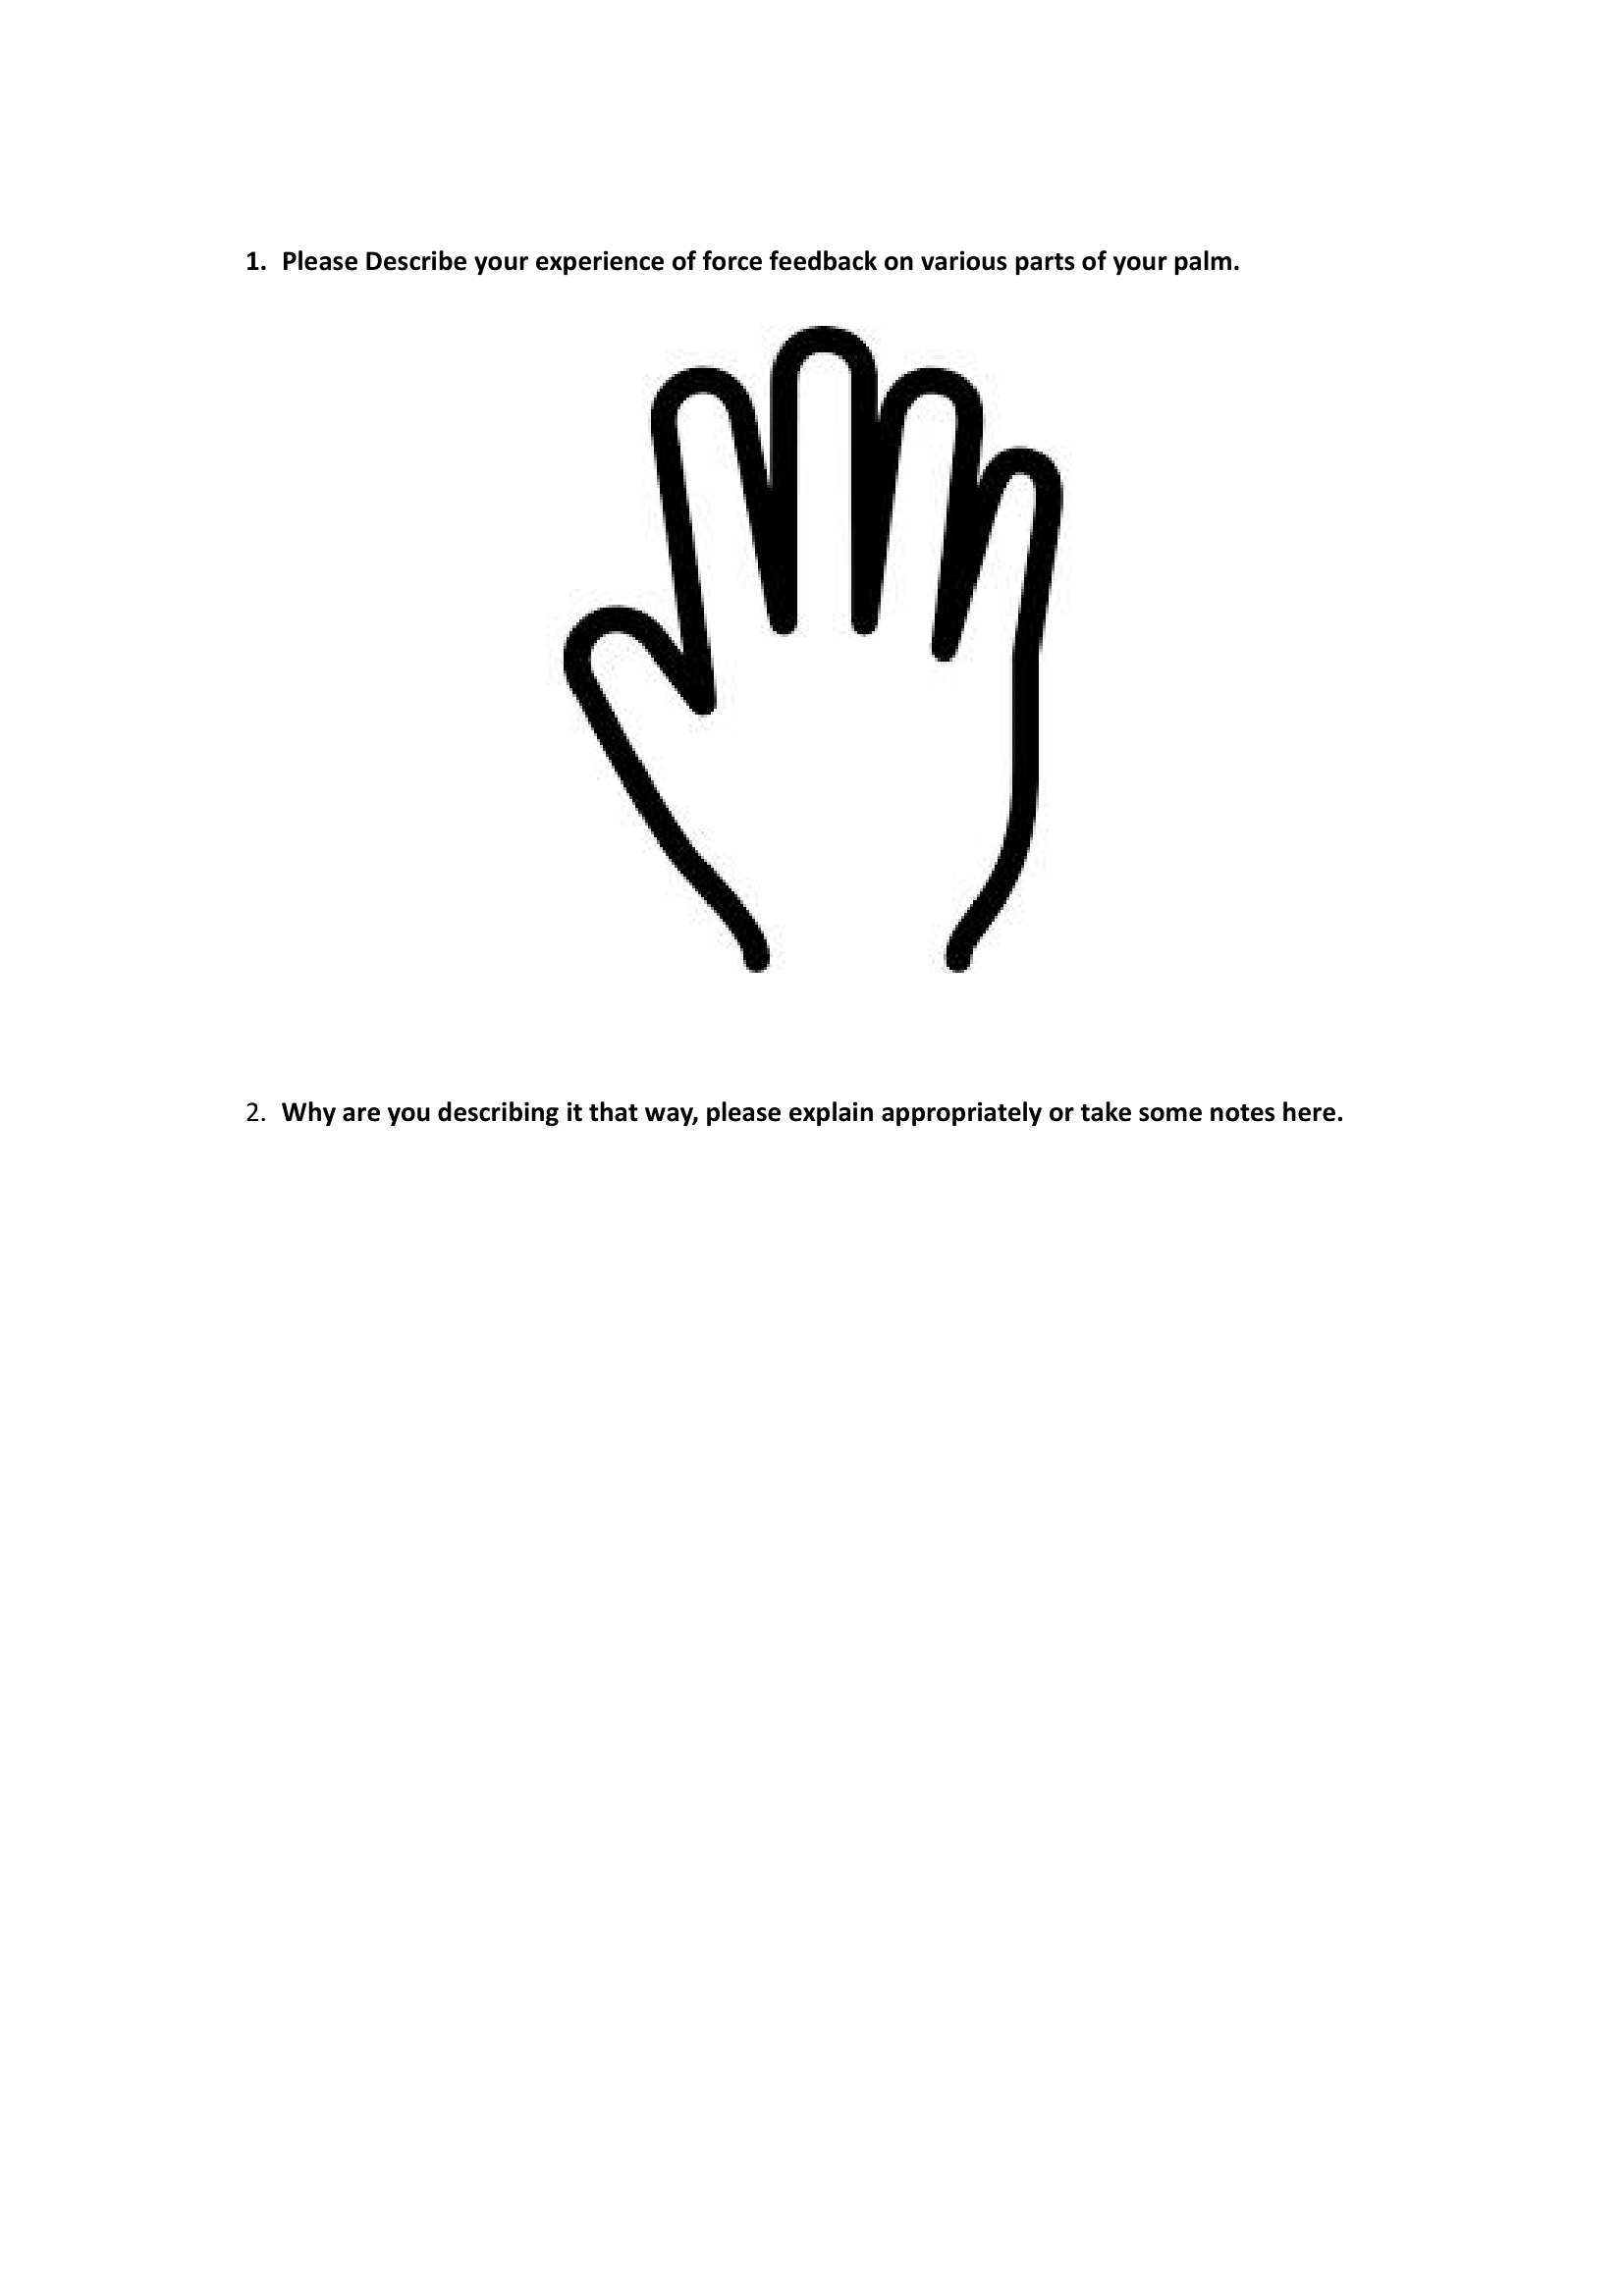
\includegraphics[width=1\textwidth,height=0.7\textheight]{A_thesis/appendix/Experiment1_questionnaire-7.png}
\end{figure}
\newpage

\section{Questionnaire of the Experiment2}
\begin{figure}[h]
\centering
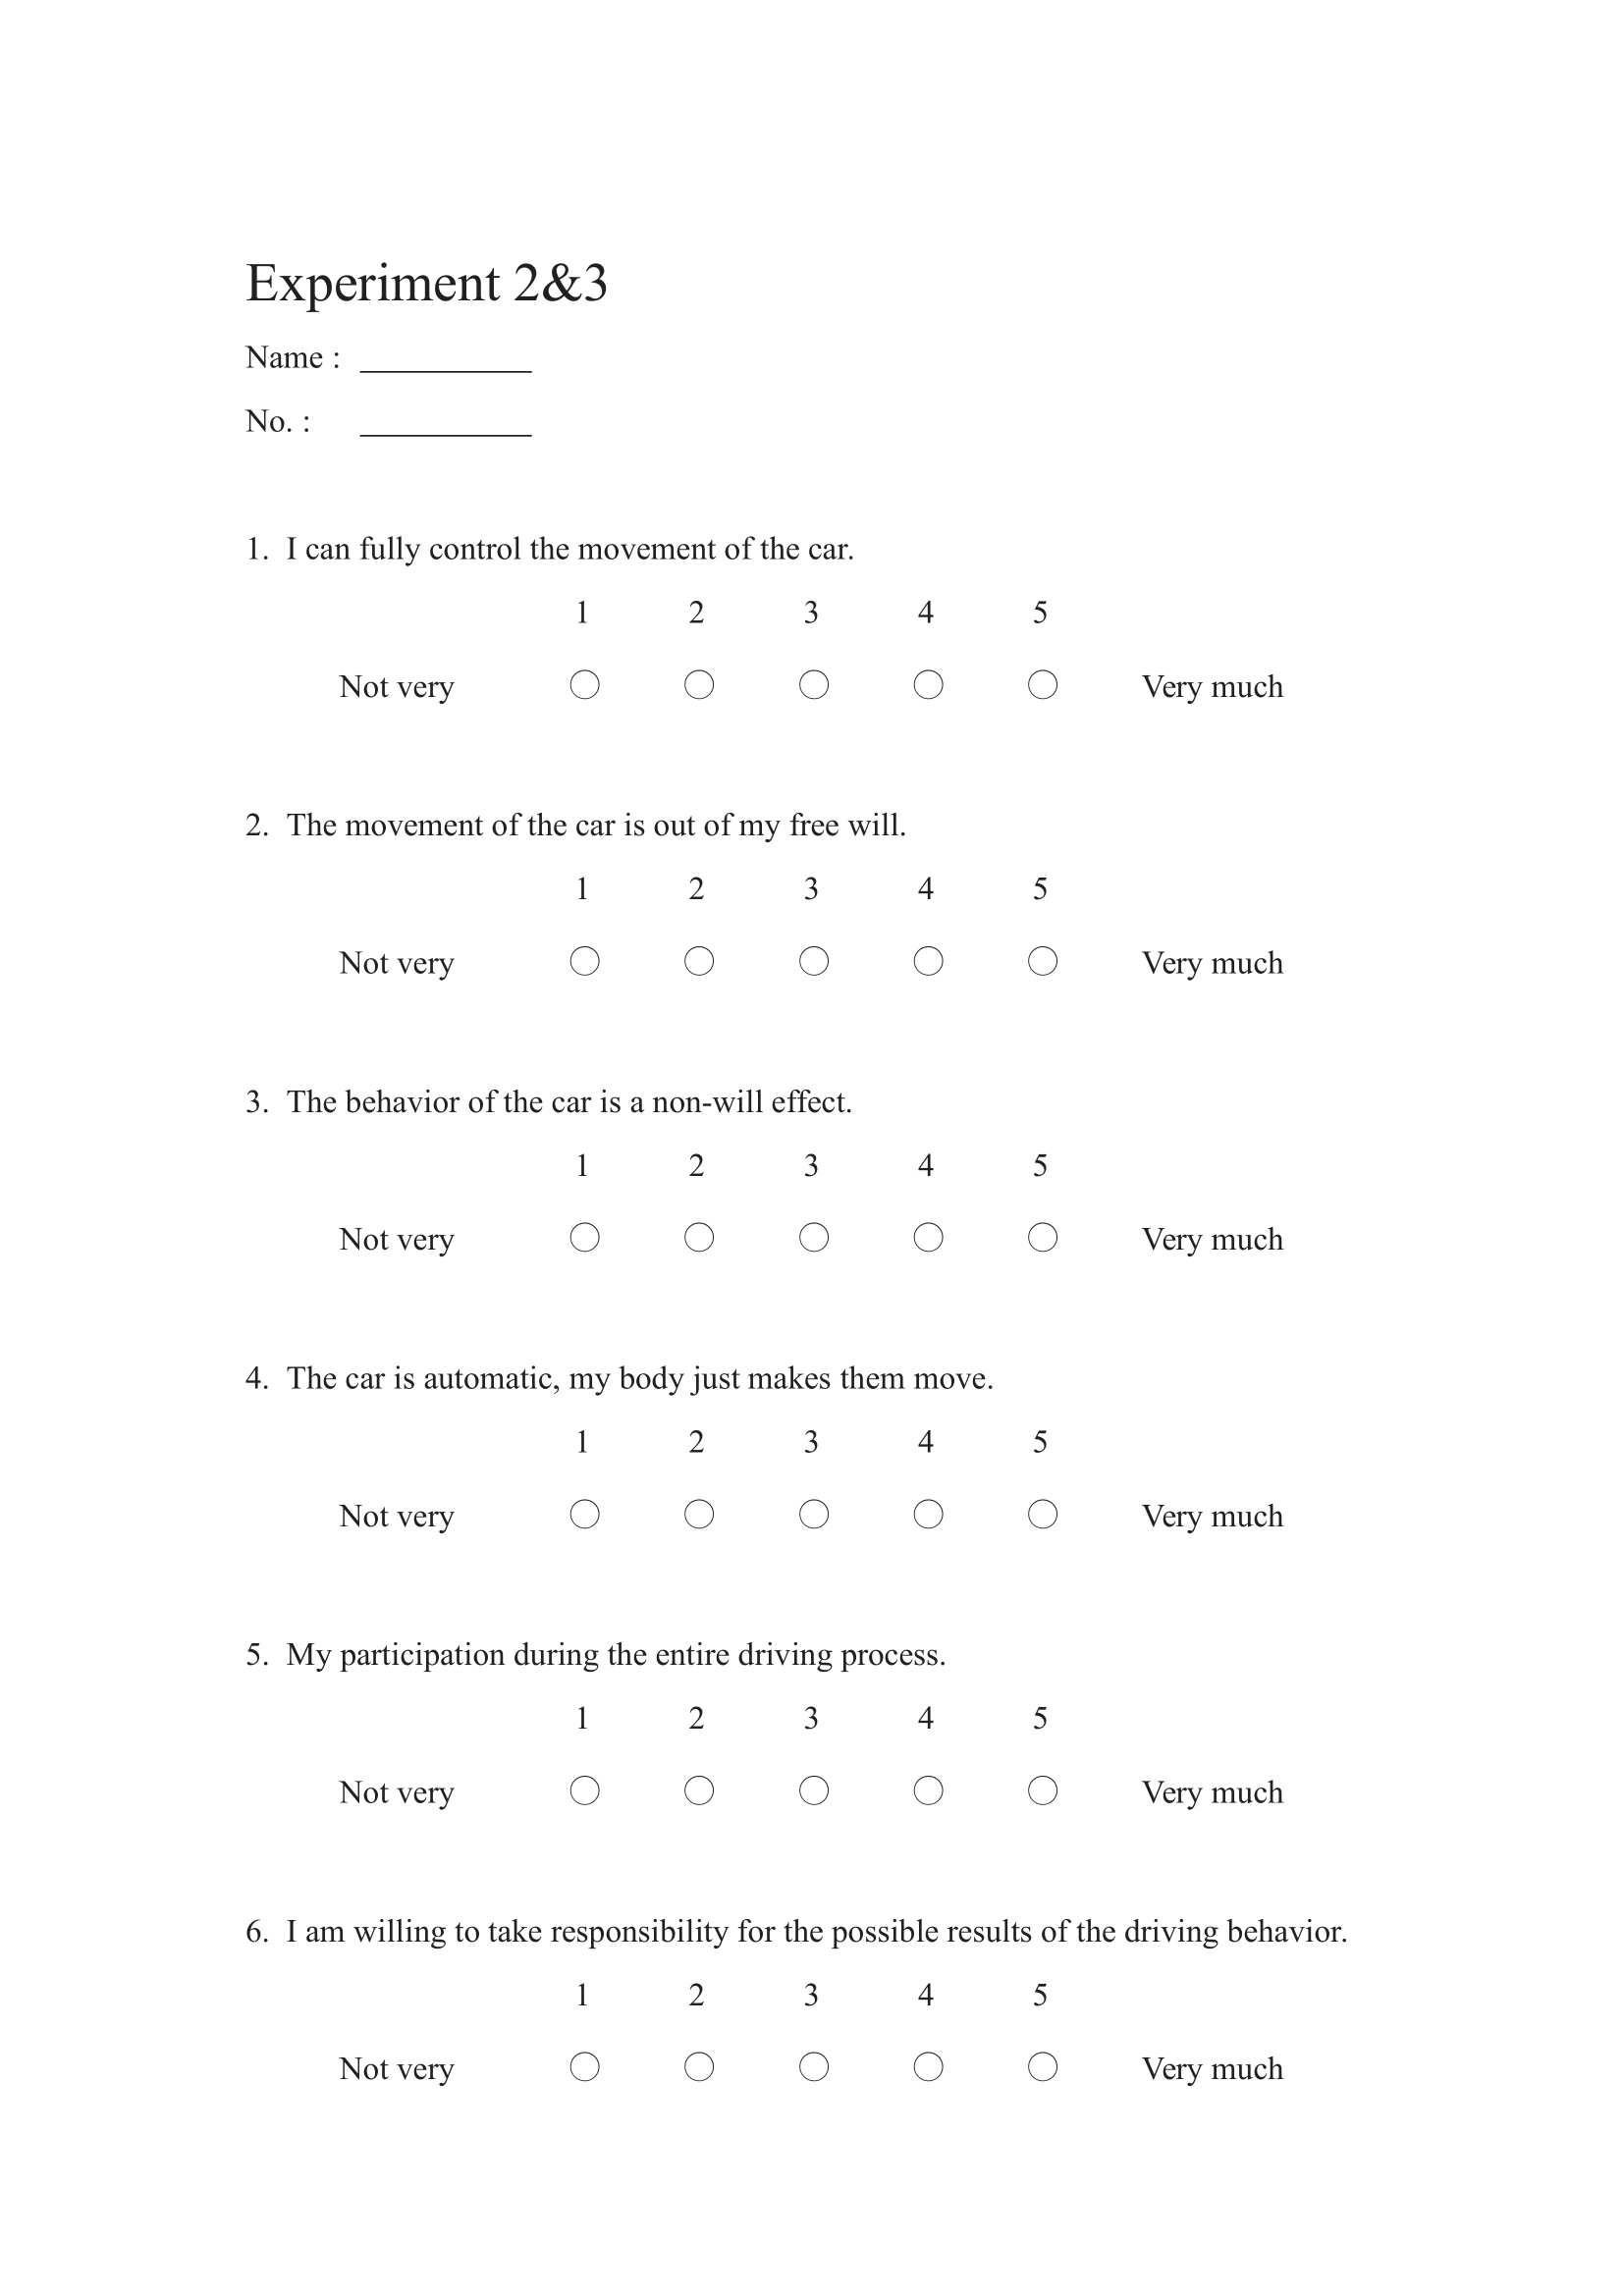
\includegraphics[width=1\textwidth,height=0.7\textheight]{A_thesis/appendix/Experiment 2 3_questionnaire-1.png}
\end{figure}
\newpage

\begin{figure}[h]
\centering
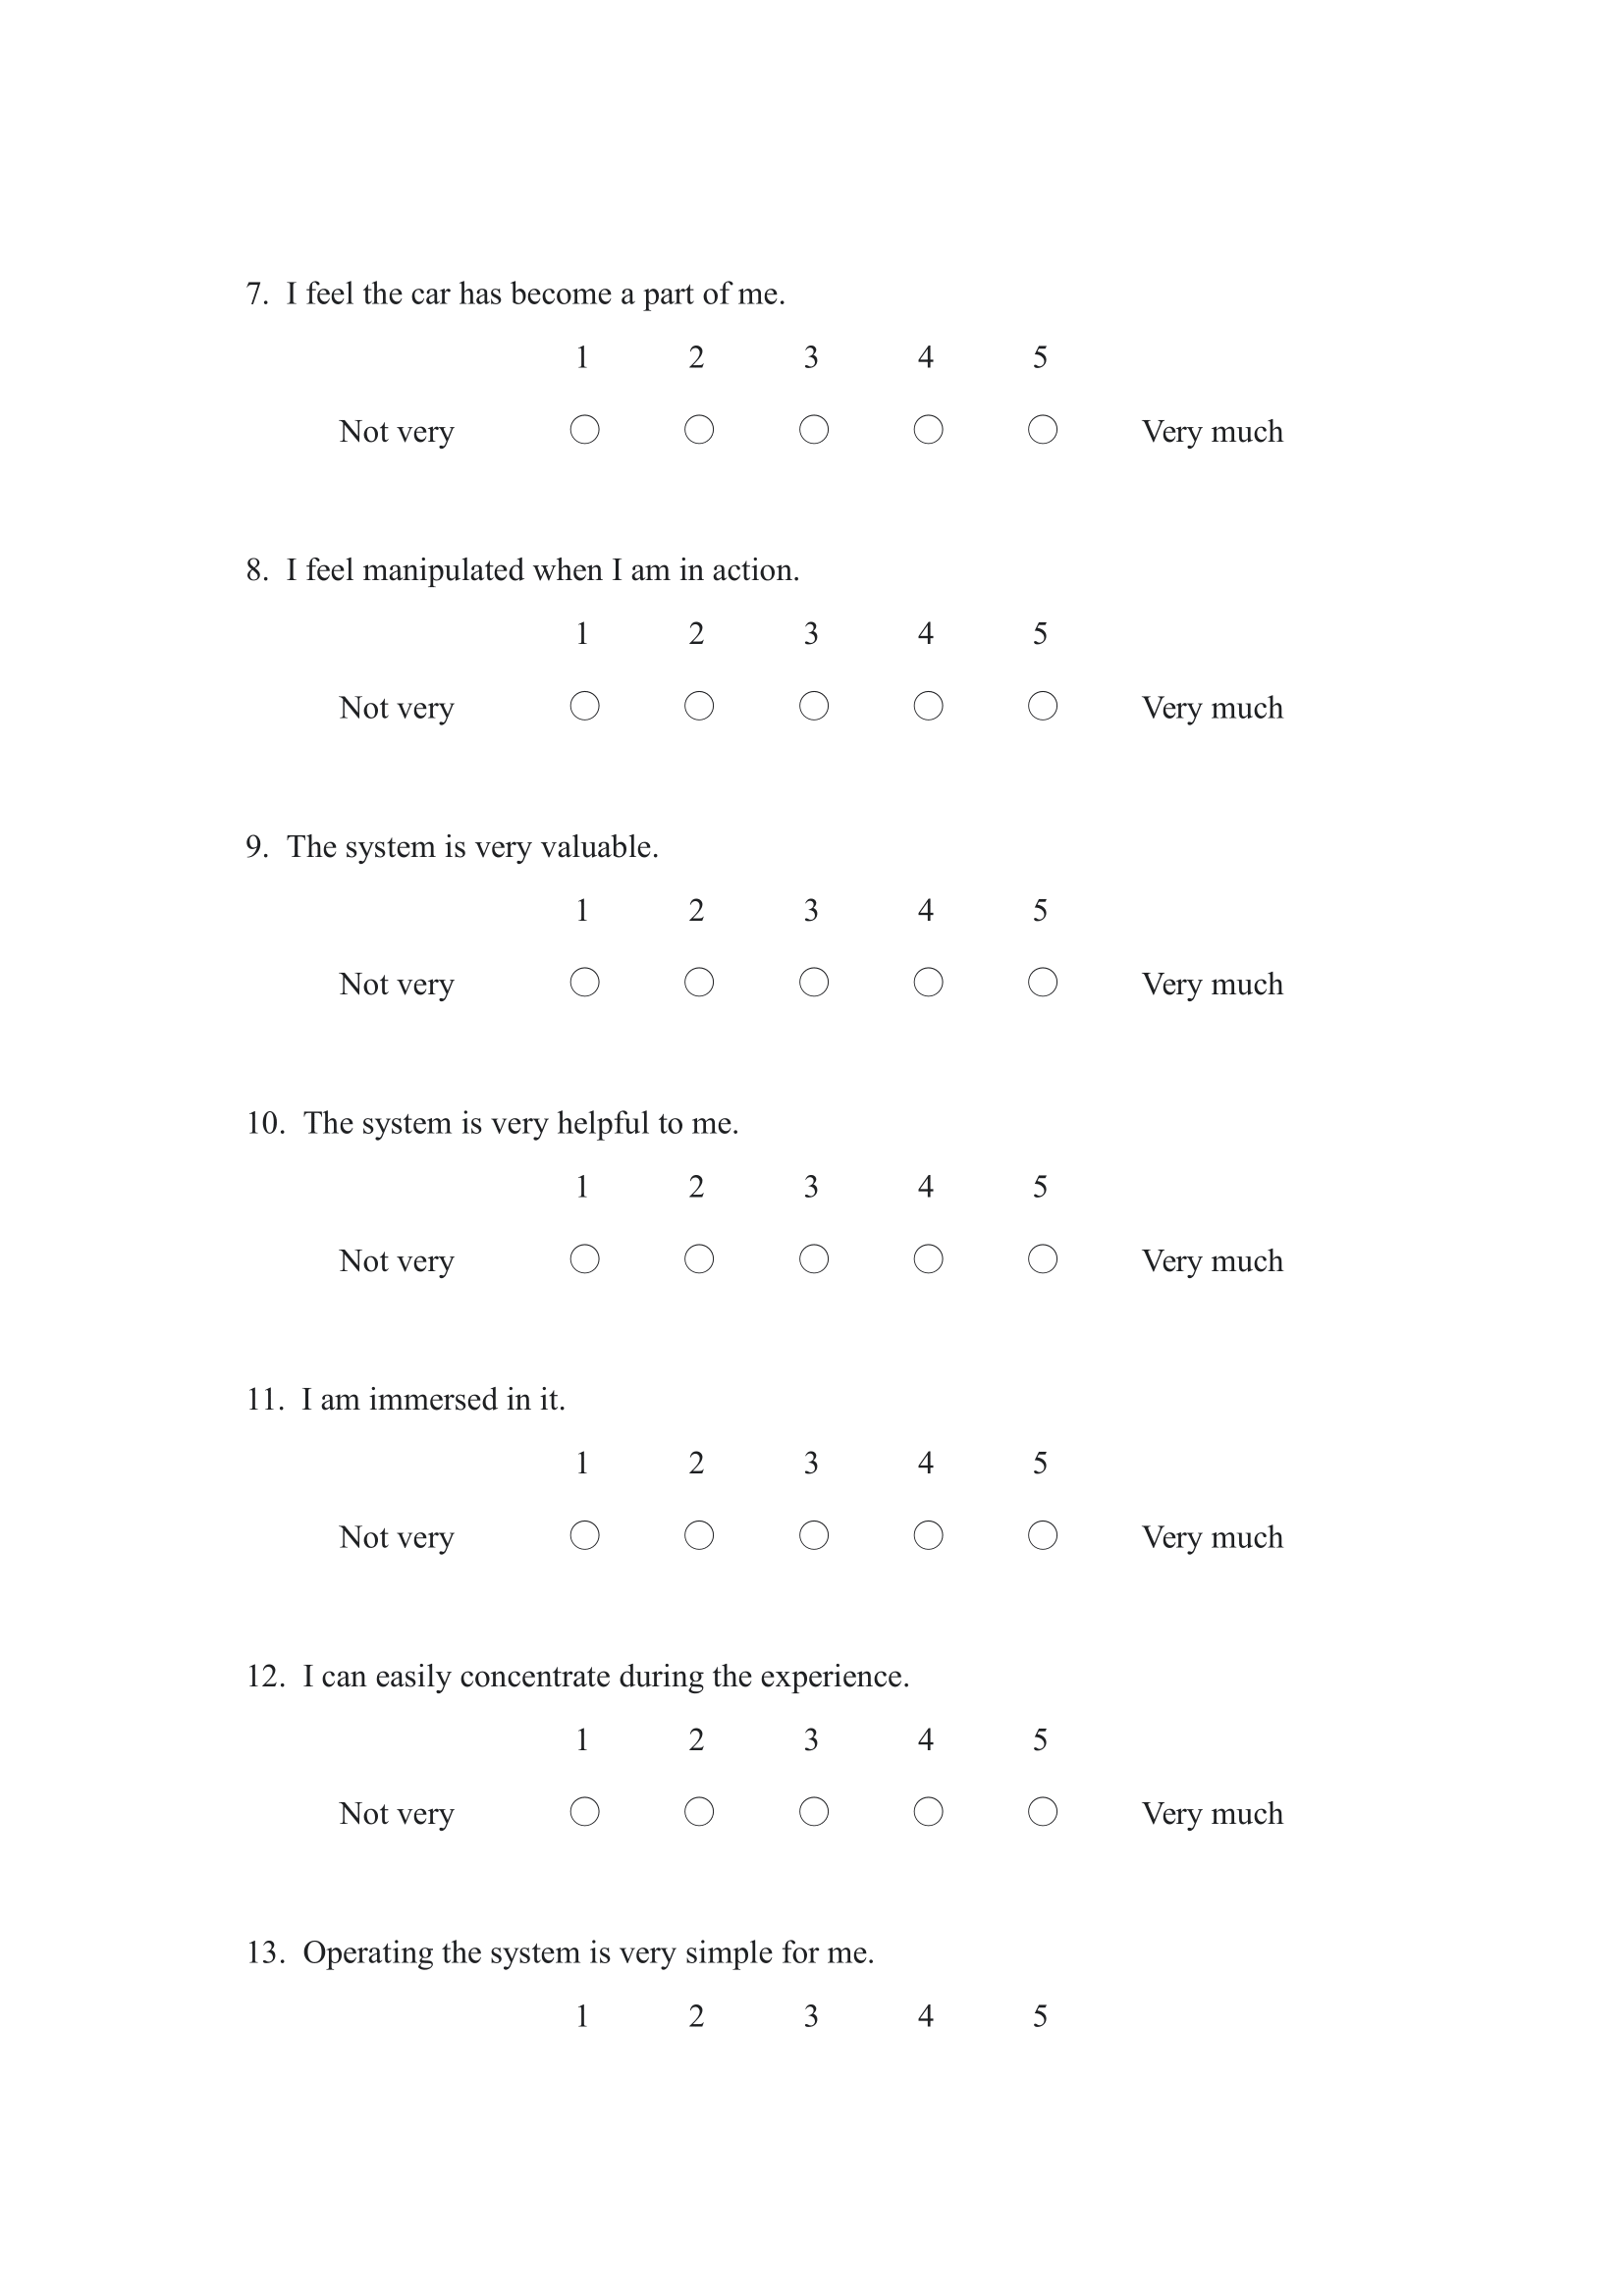
\includegraphics[width=1\textwidth,height=0.7\textheight]{A_thesis/appendix/Experiment 2 3_questionnaire-2.png}
\end{figure}
\newpage

\begin{figure}[h]
\centering
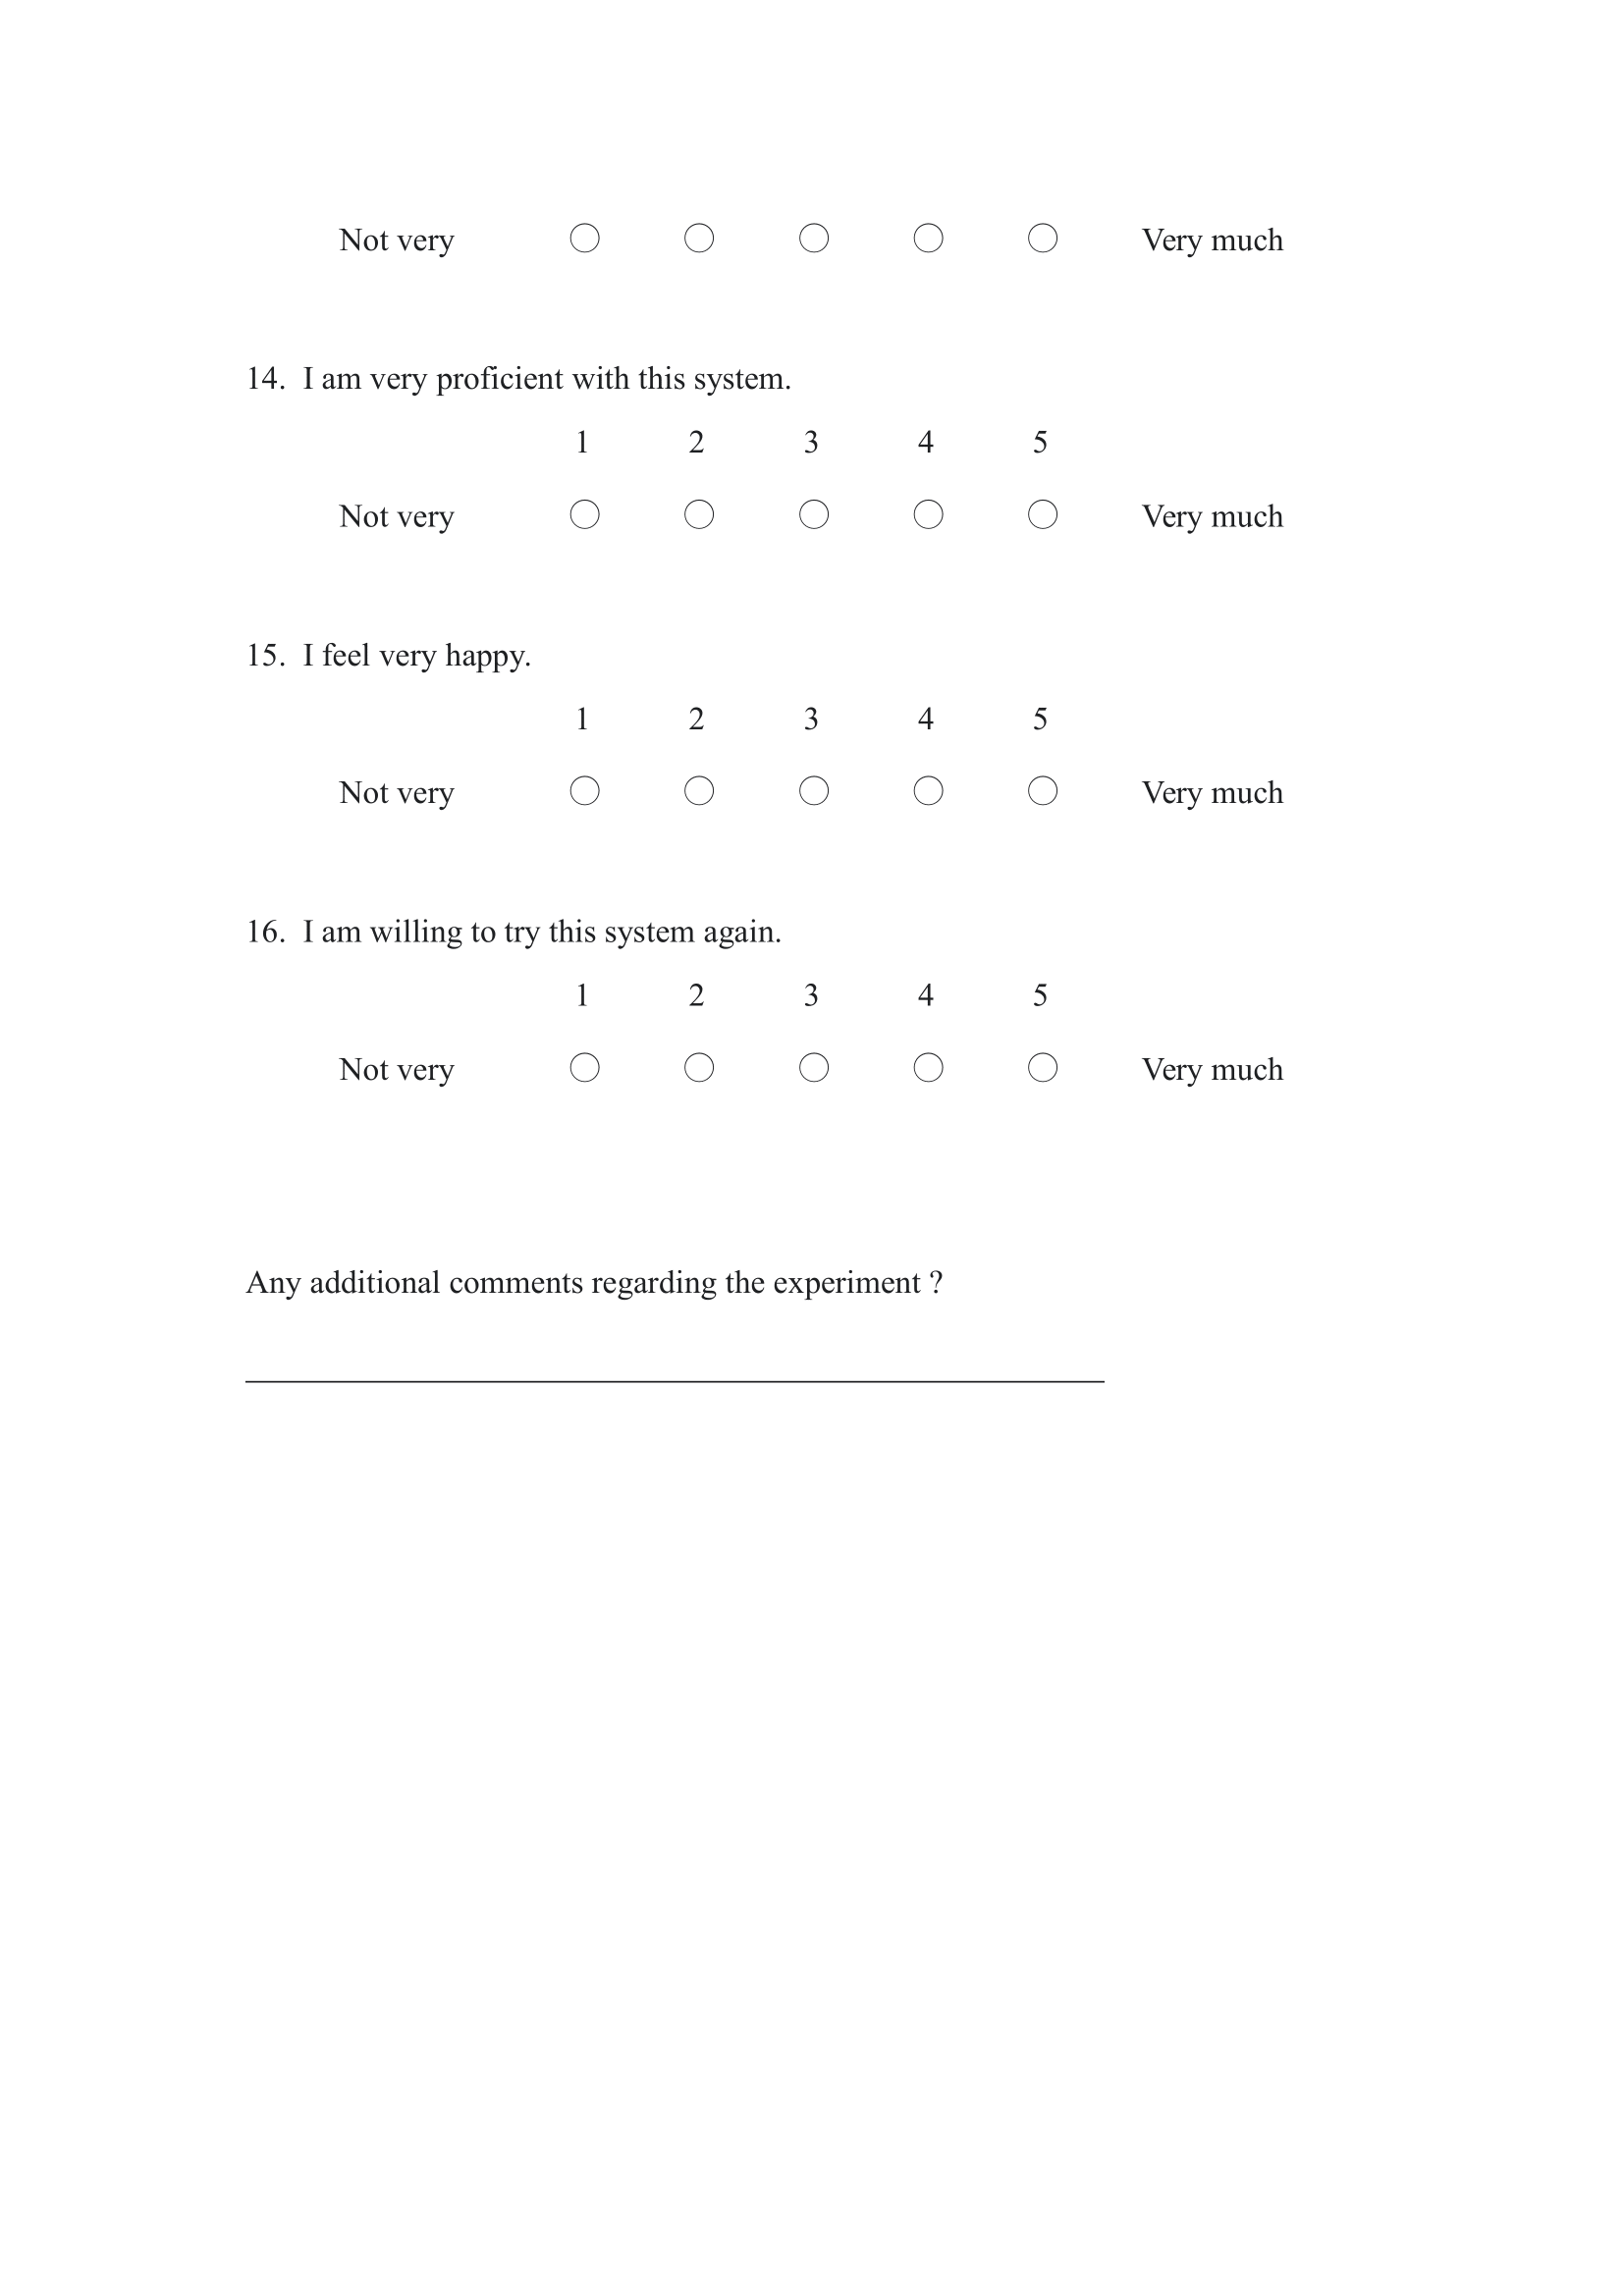
\includegraphics[width=1\textwidth,height=0.7\textheight]{A_thesis/appendix/Experiment 2 3_questionnaire-3.png}
\end{figure}
\newpage

\section{Motion Information Diagram Result}
\begin{figure}[h]
\centering
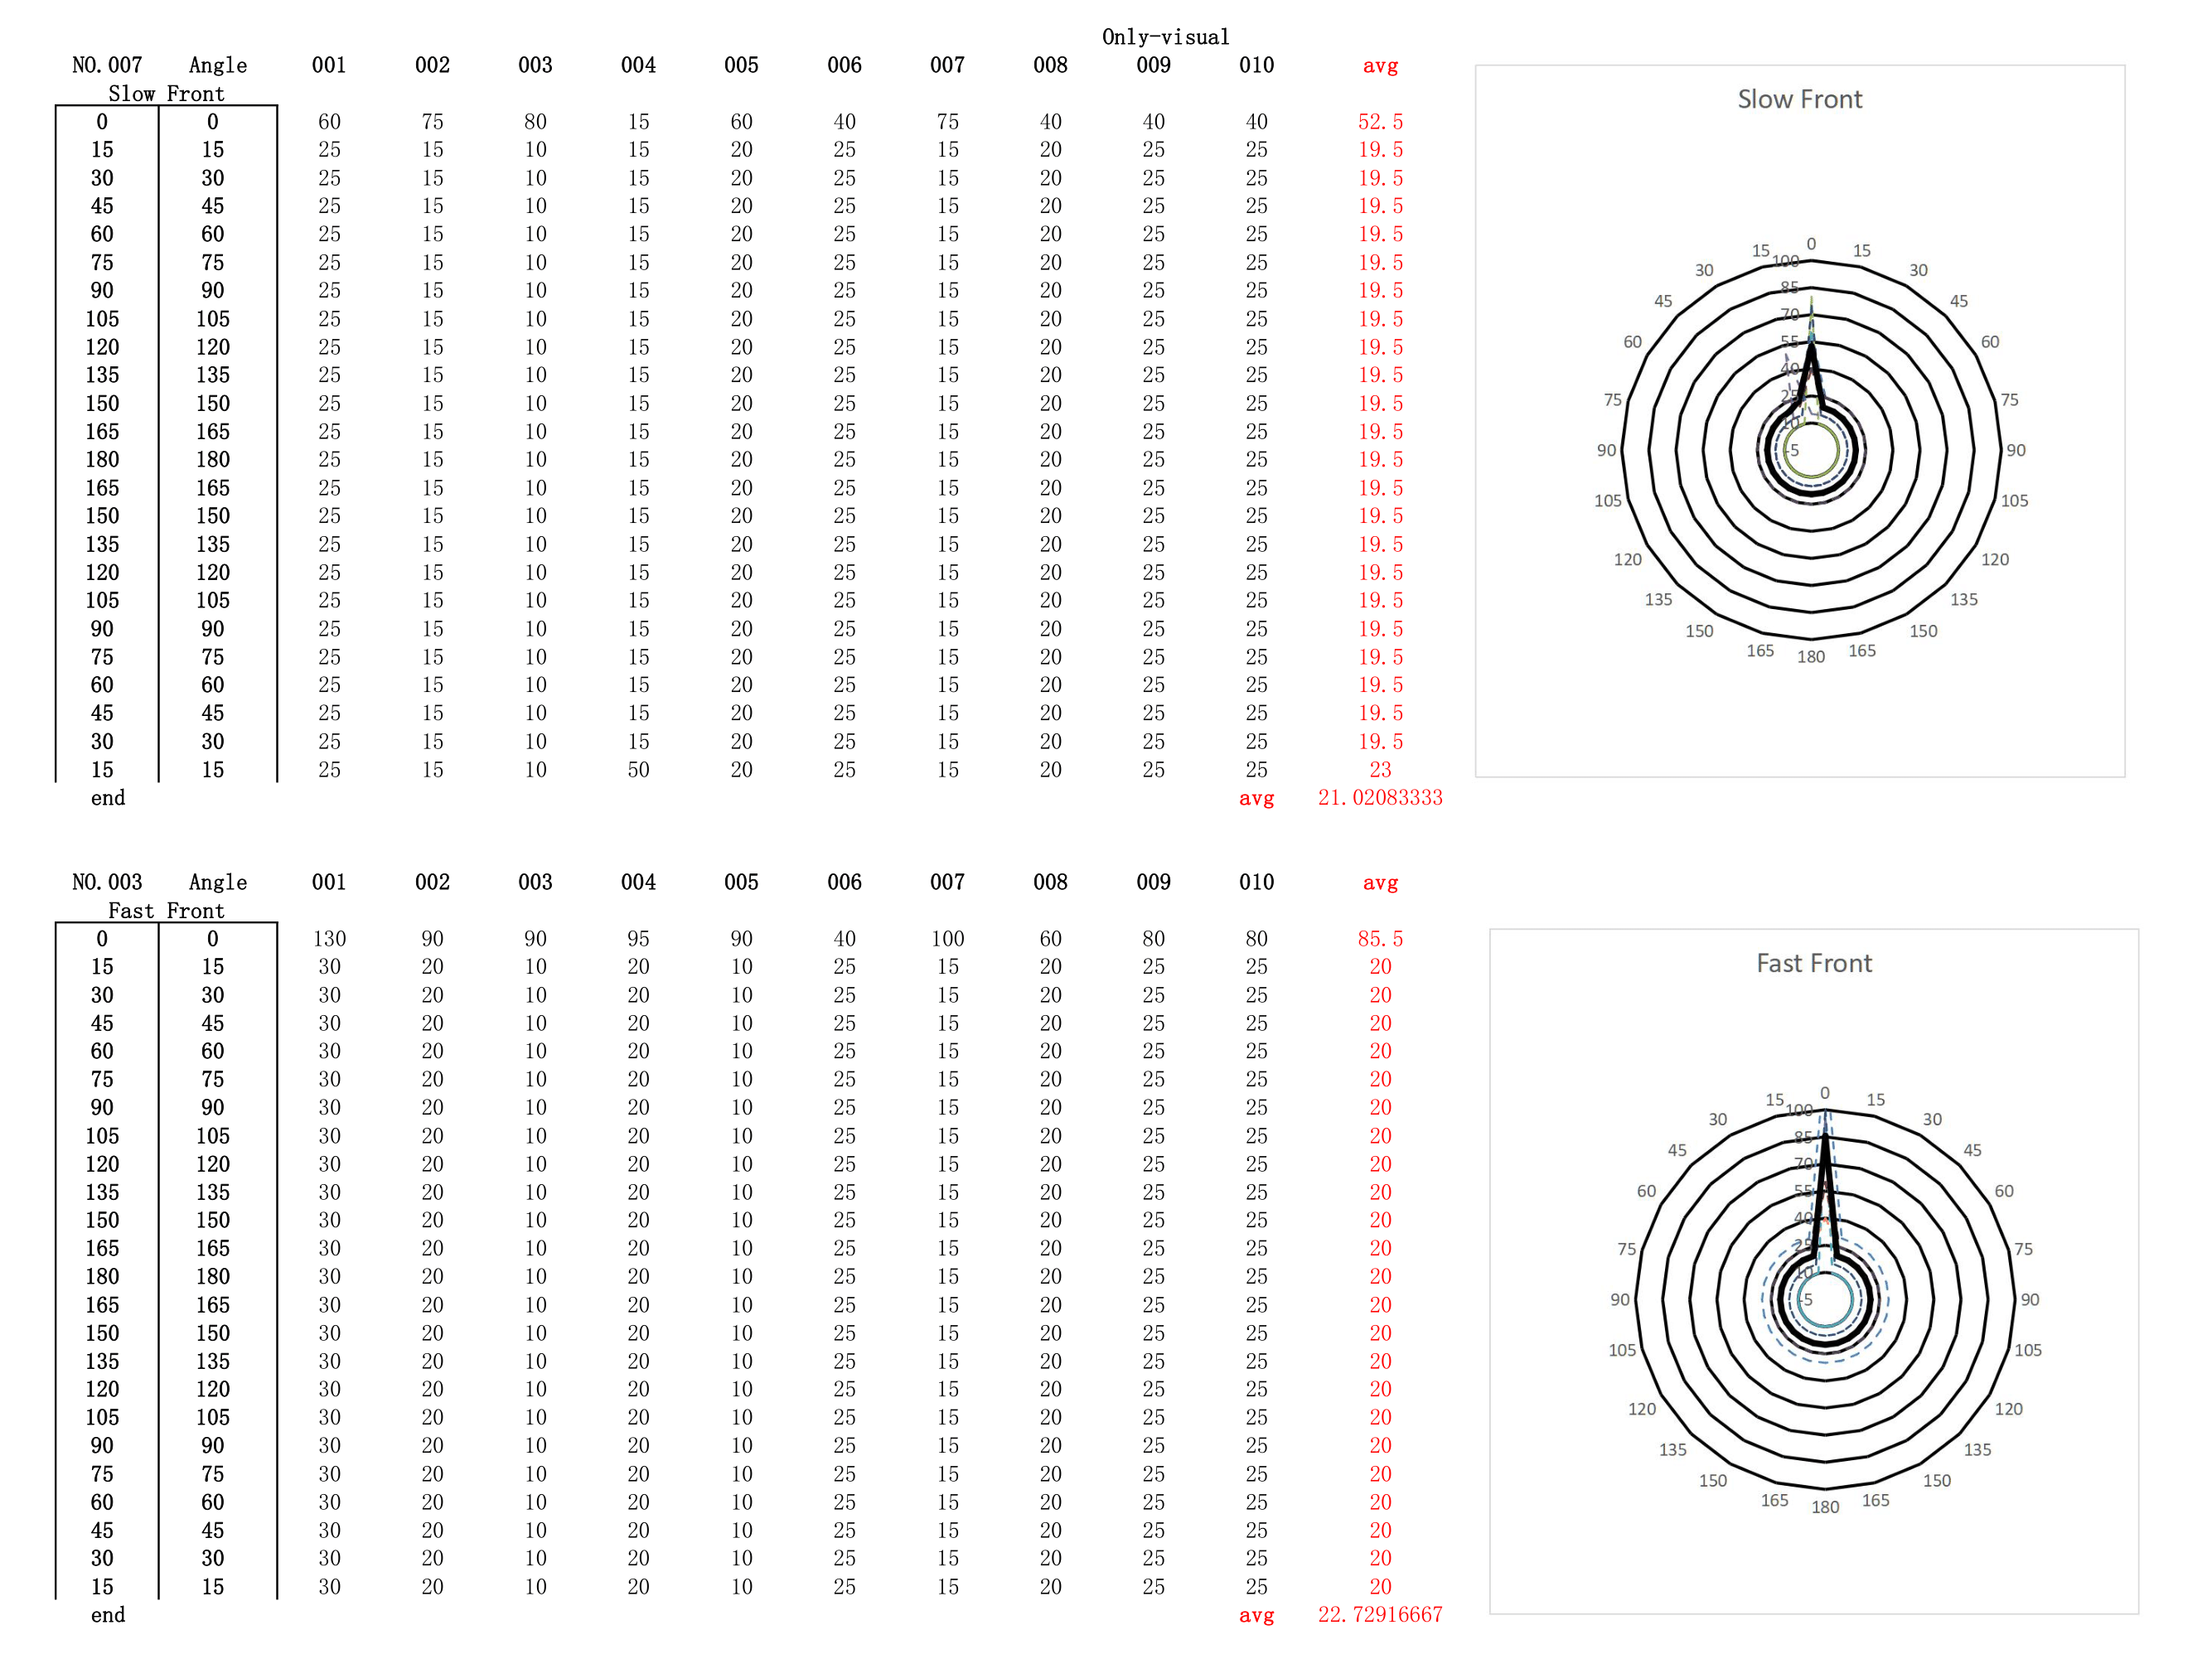
\includegraphics[width=0.9\textwidth,height=0.36\textheight]{A_thesis/appendix/Exp1_1-01.png}
\break
\break
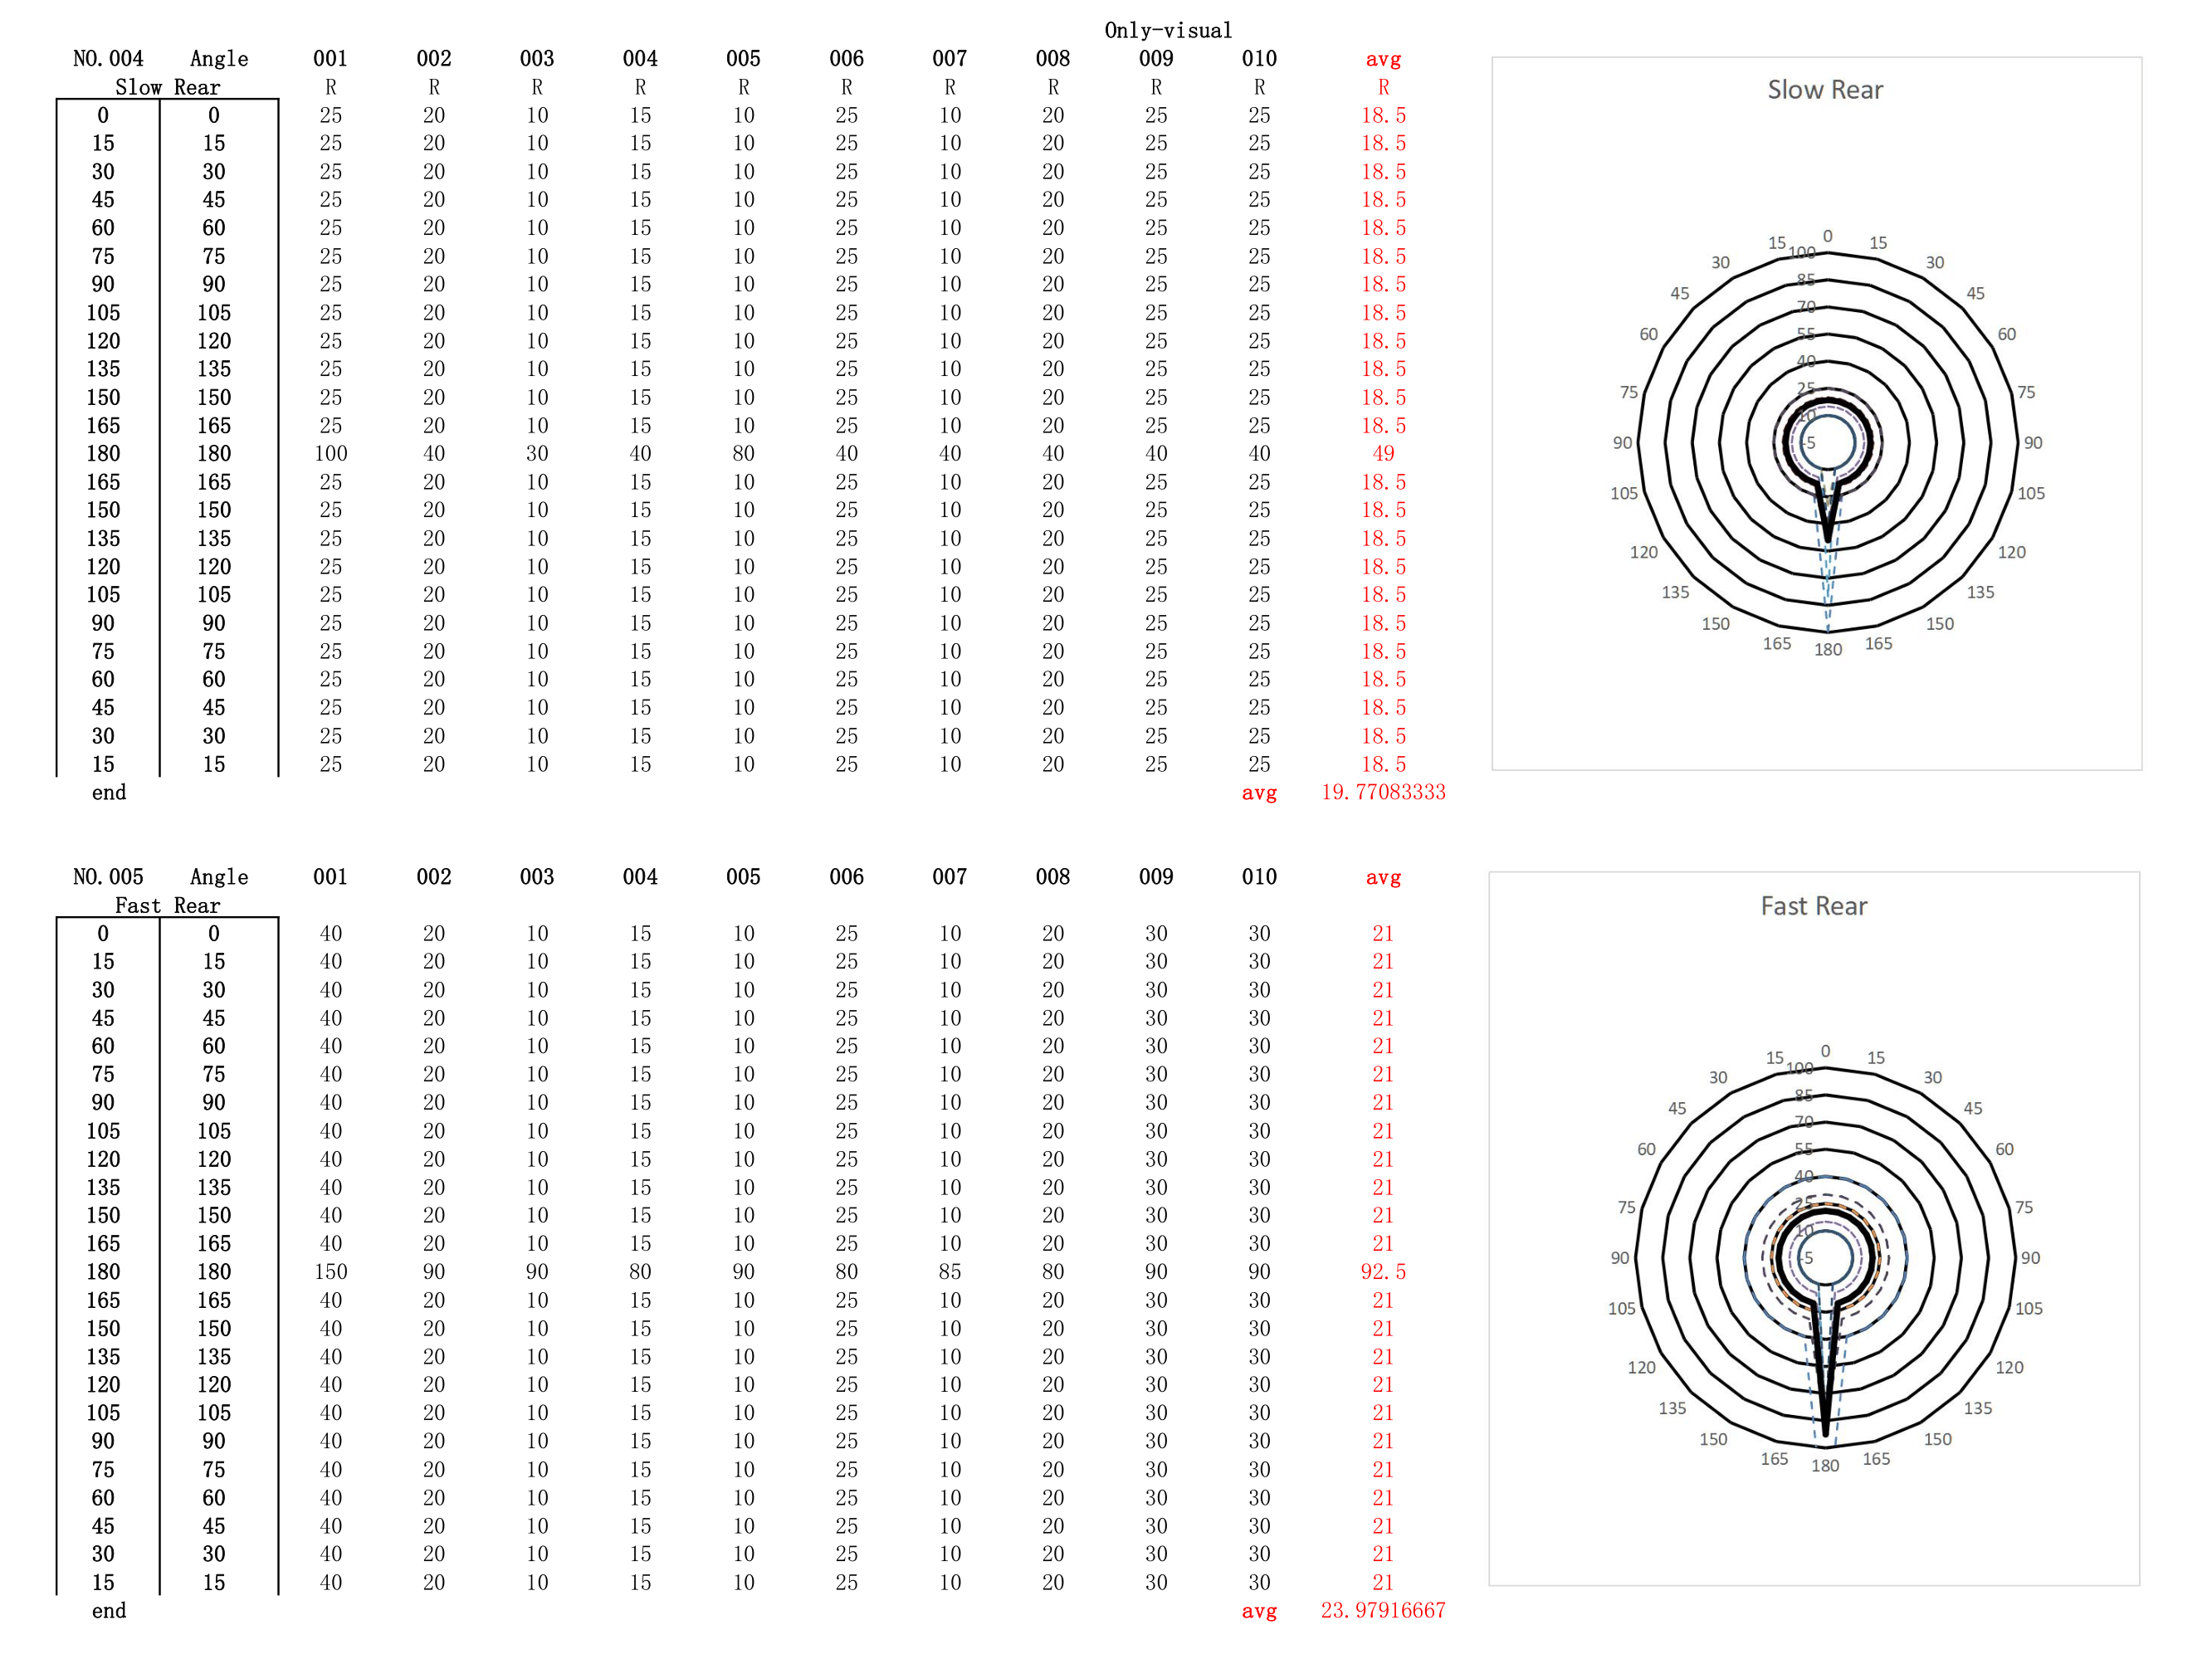
\includegraphics[width=0.9\textwidth,height=0.36\textheight]{A_thesis/appendix/Exp1_1-02.png}
\end{figure}
\newpage

\begin{figure}[h]
\centering
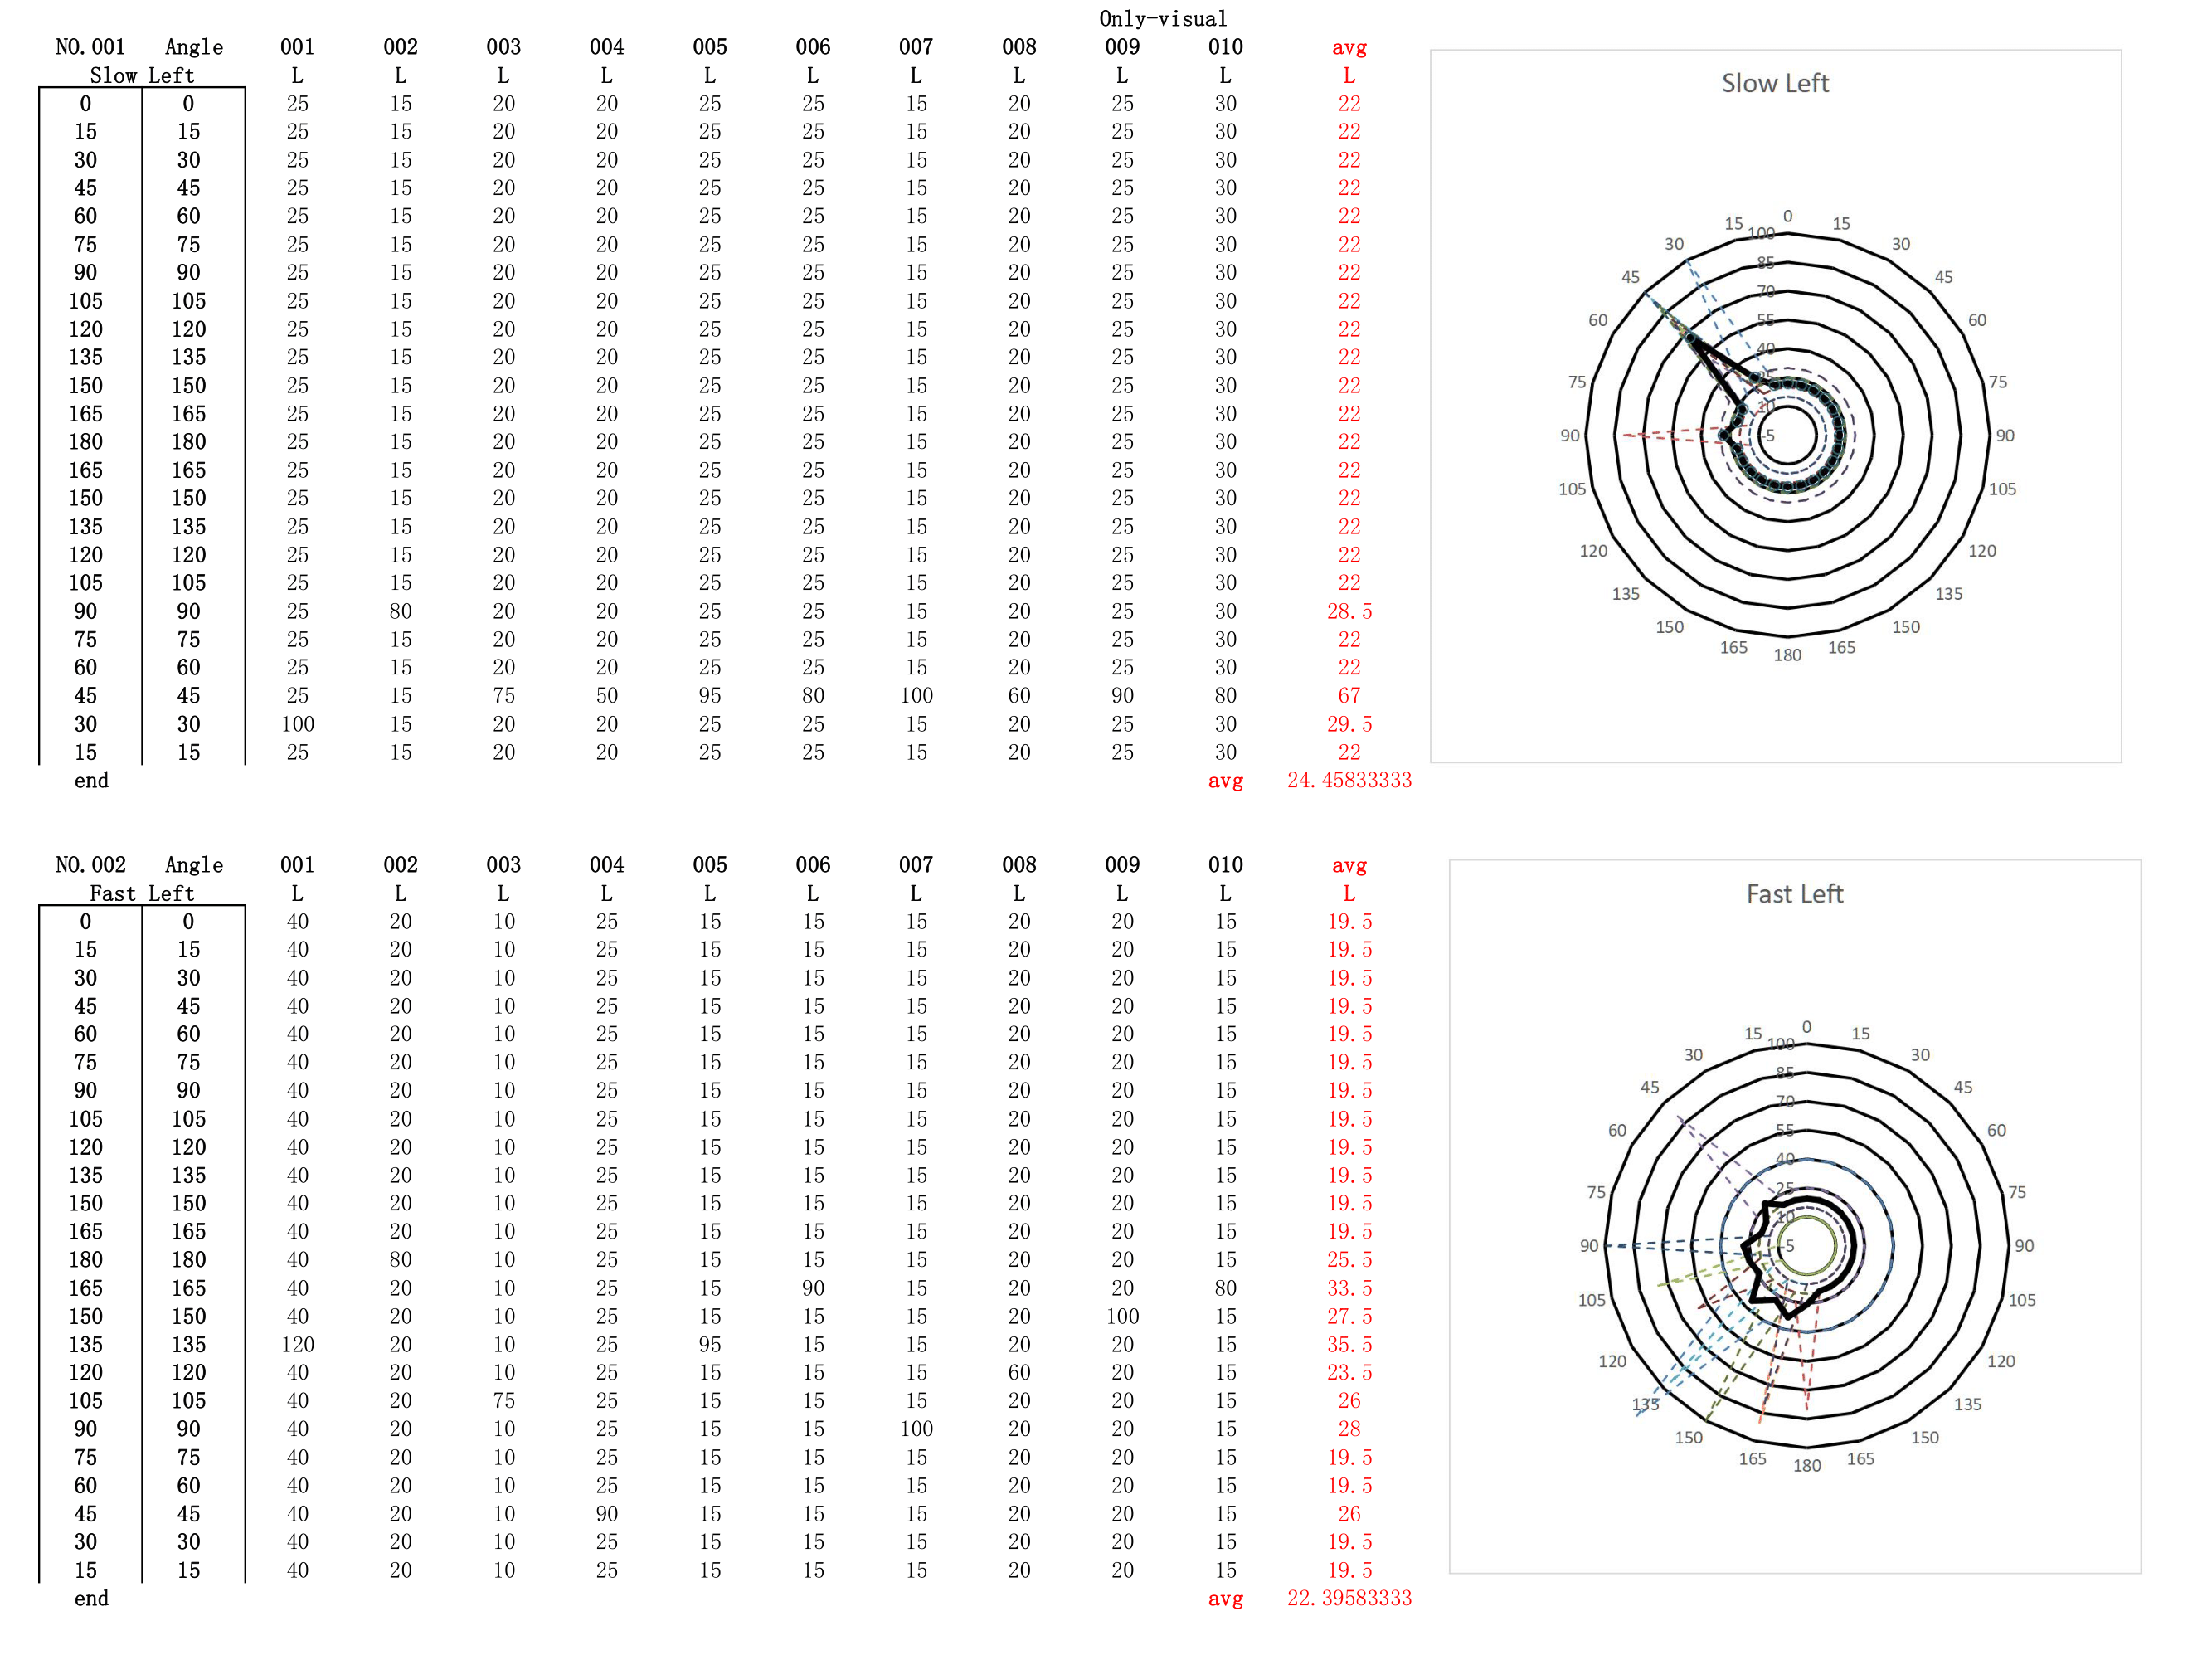
\includegraphics[width=0.9\textwidth,height=0.36\textheight]{A_thesis/appendix/Exp1_1-03.png}
\break
\break
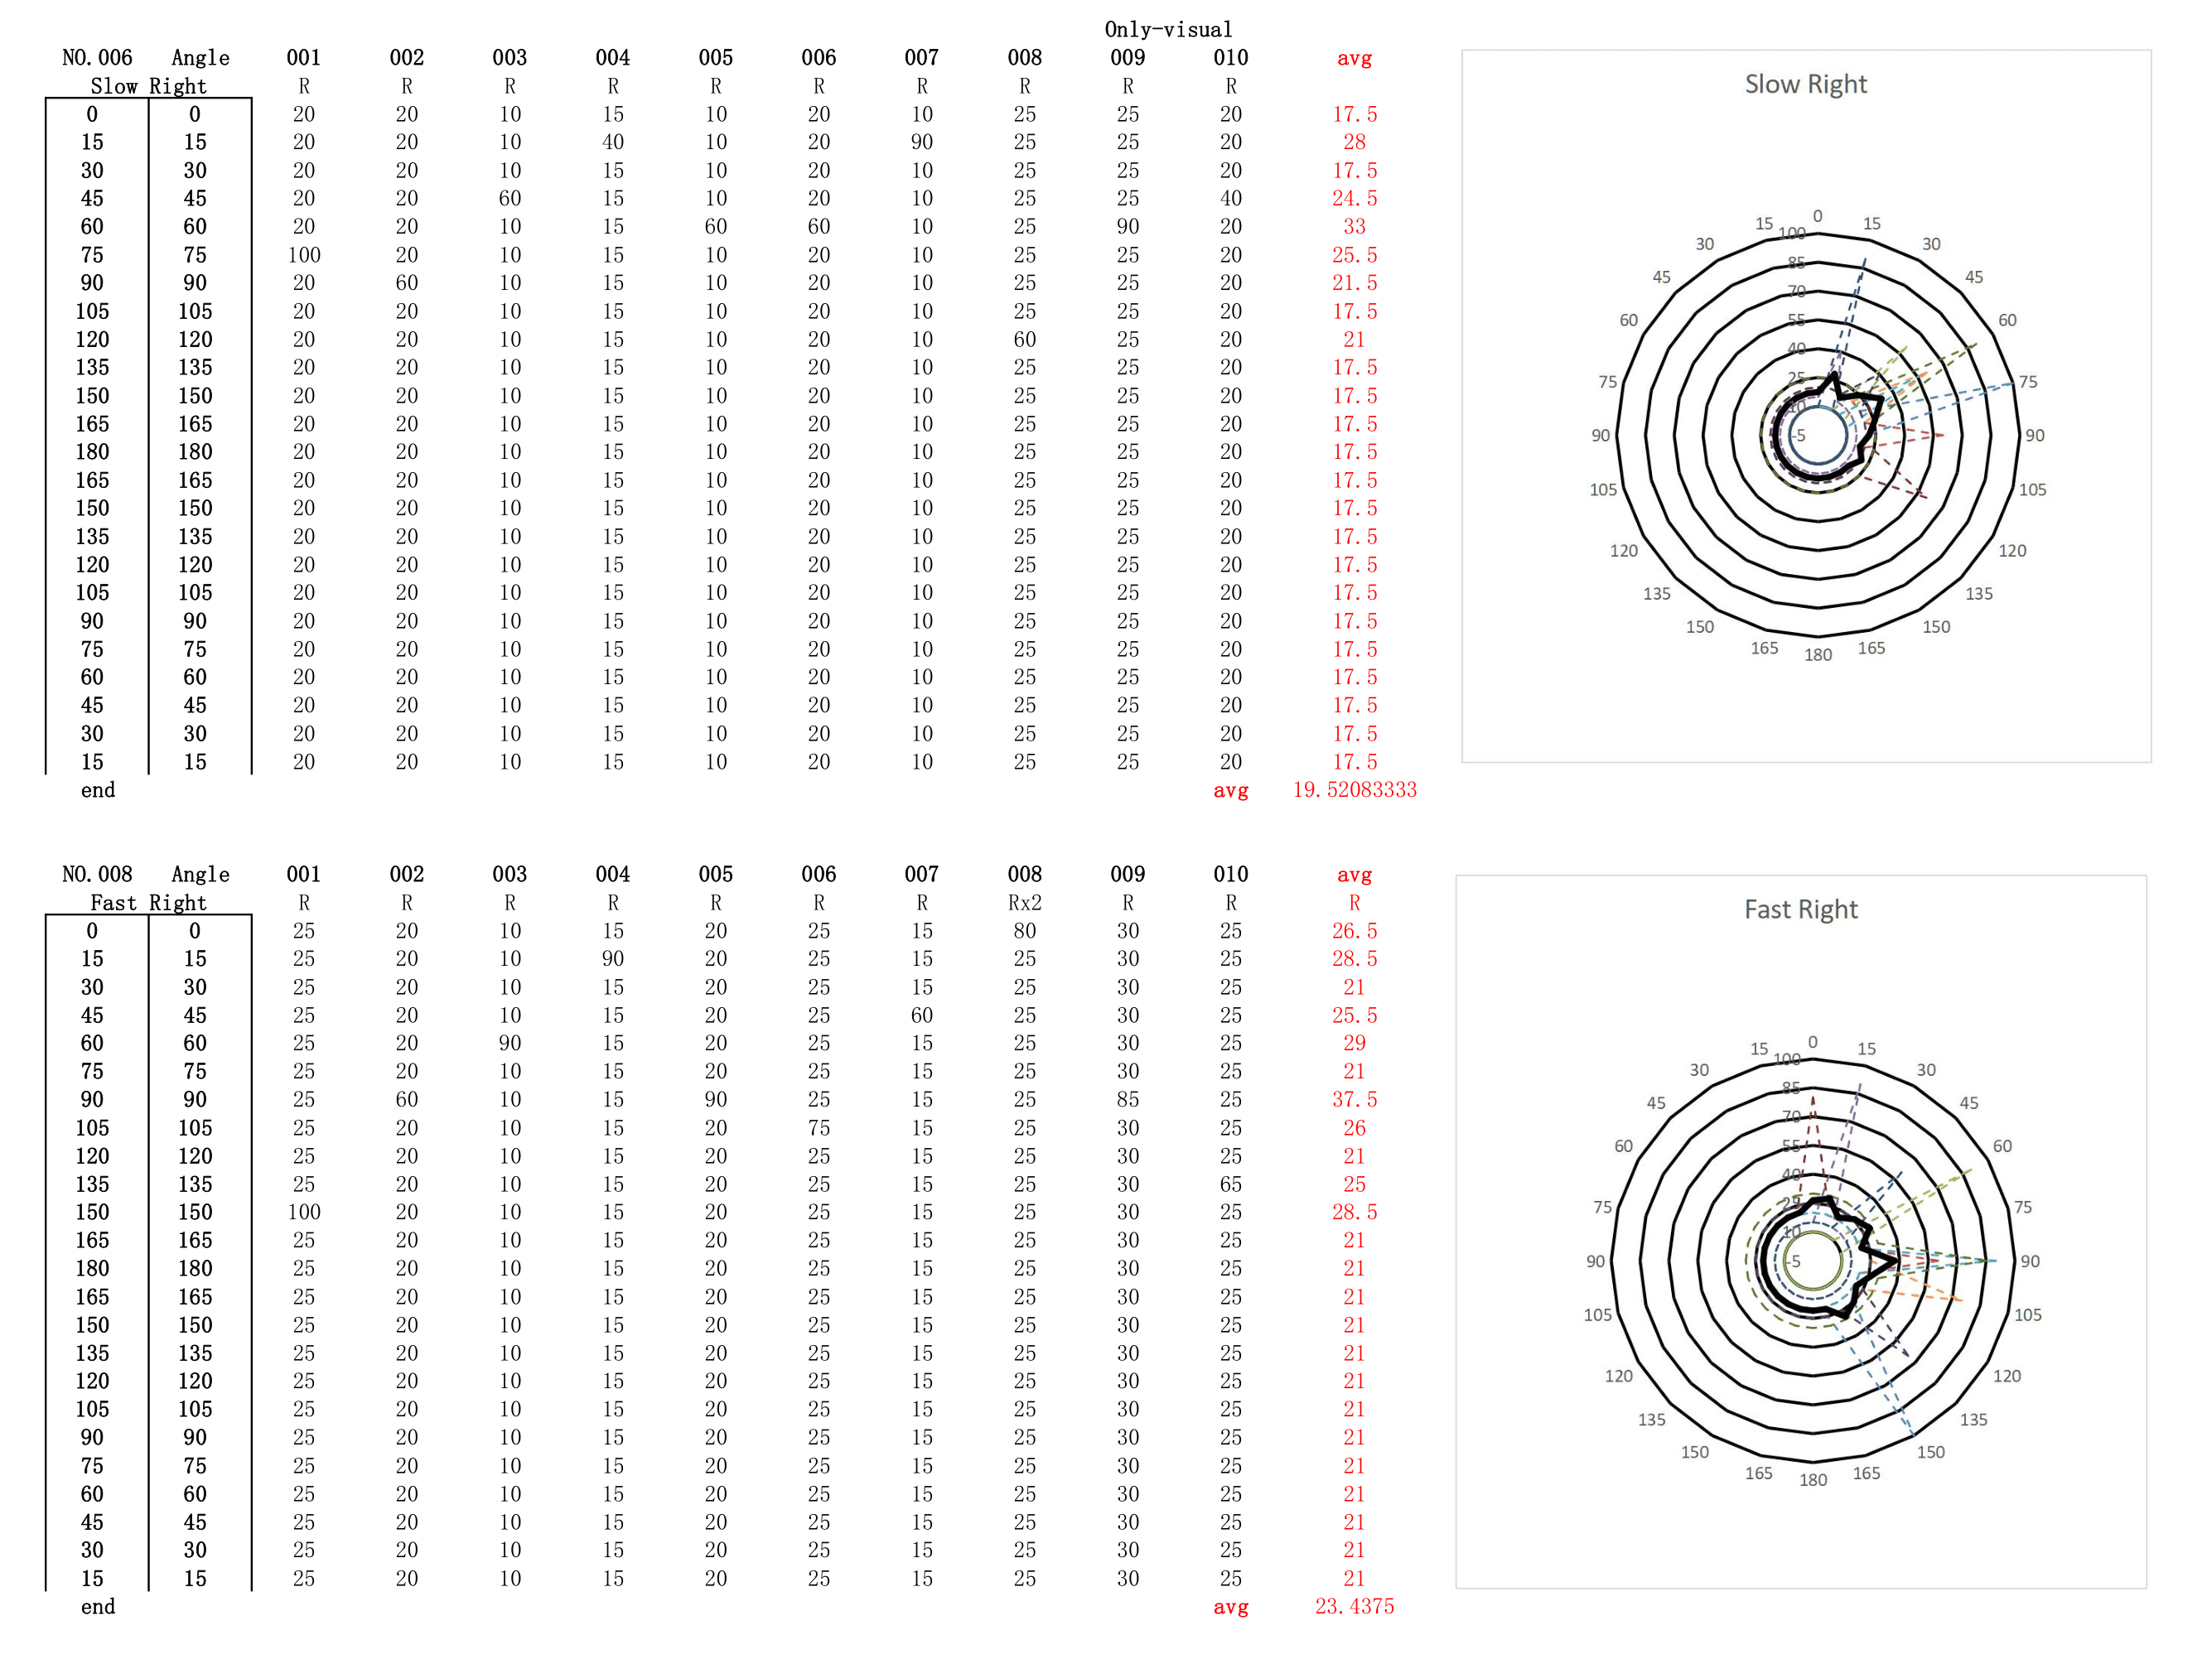
\includegraphics[width=0.9\textwidth,height=0.36\textheight]{A_thesis/appendix/Exp1_1-04.png}
\end{figure}
\newpage

\begin{figure}[h]
\centering
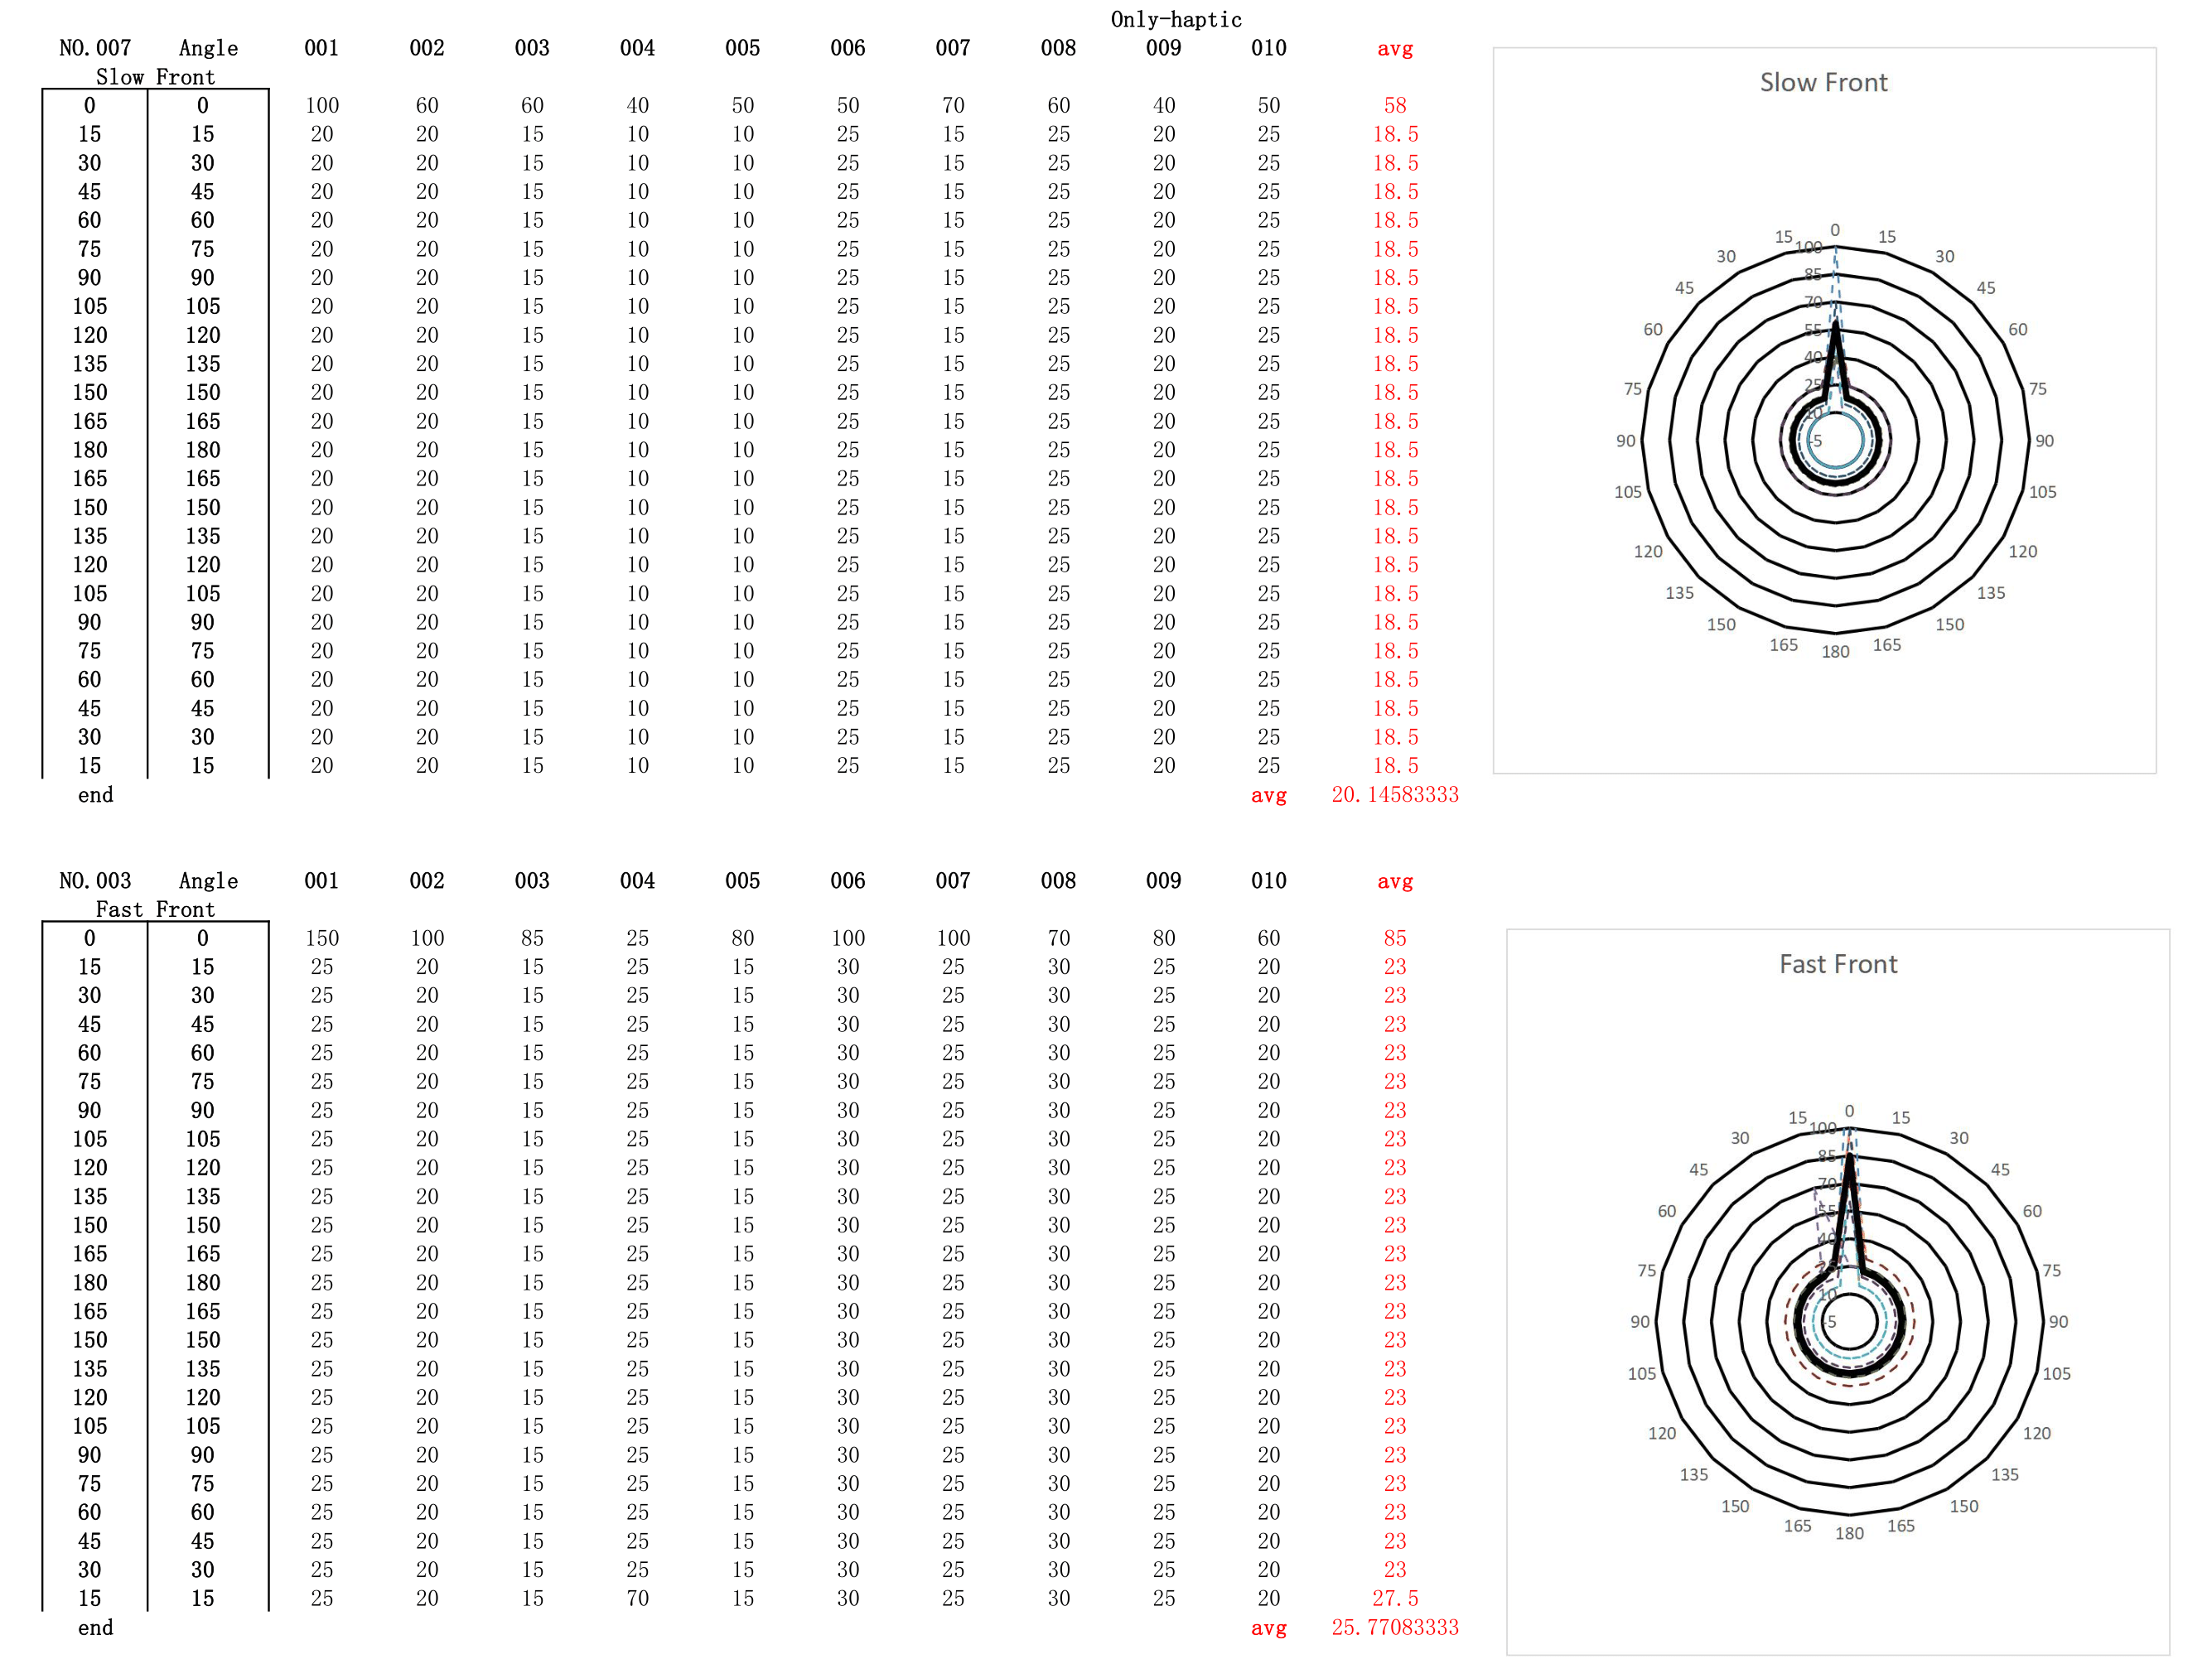
\includegraphics[width=0.9\textwidth,height=0.36\textheight]{A_thesis/appendix/Exp1_1-05.png}
\break
\break
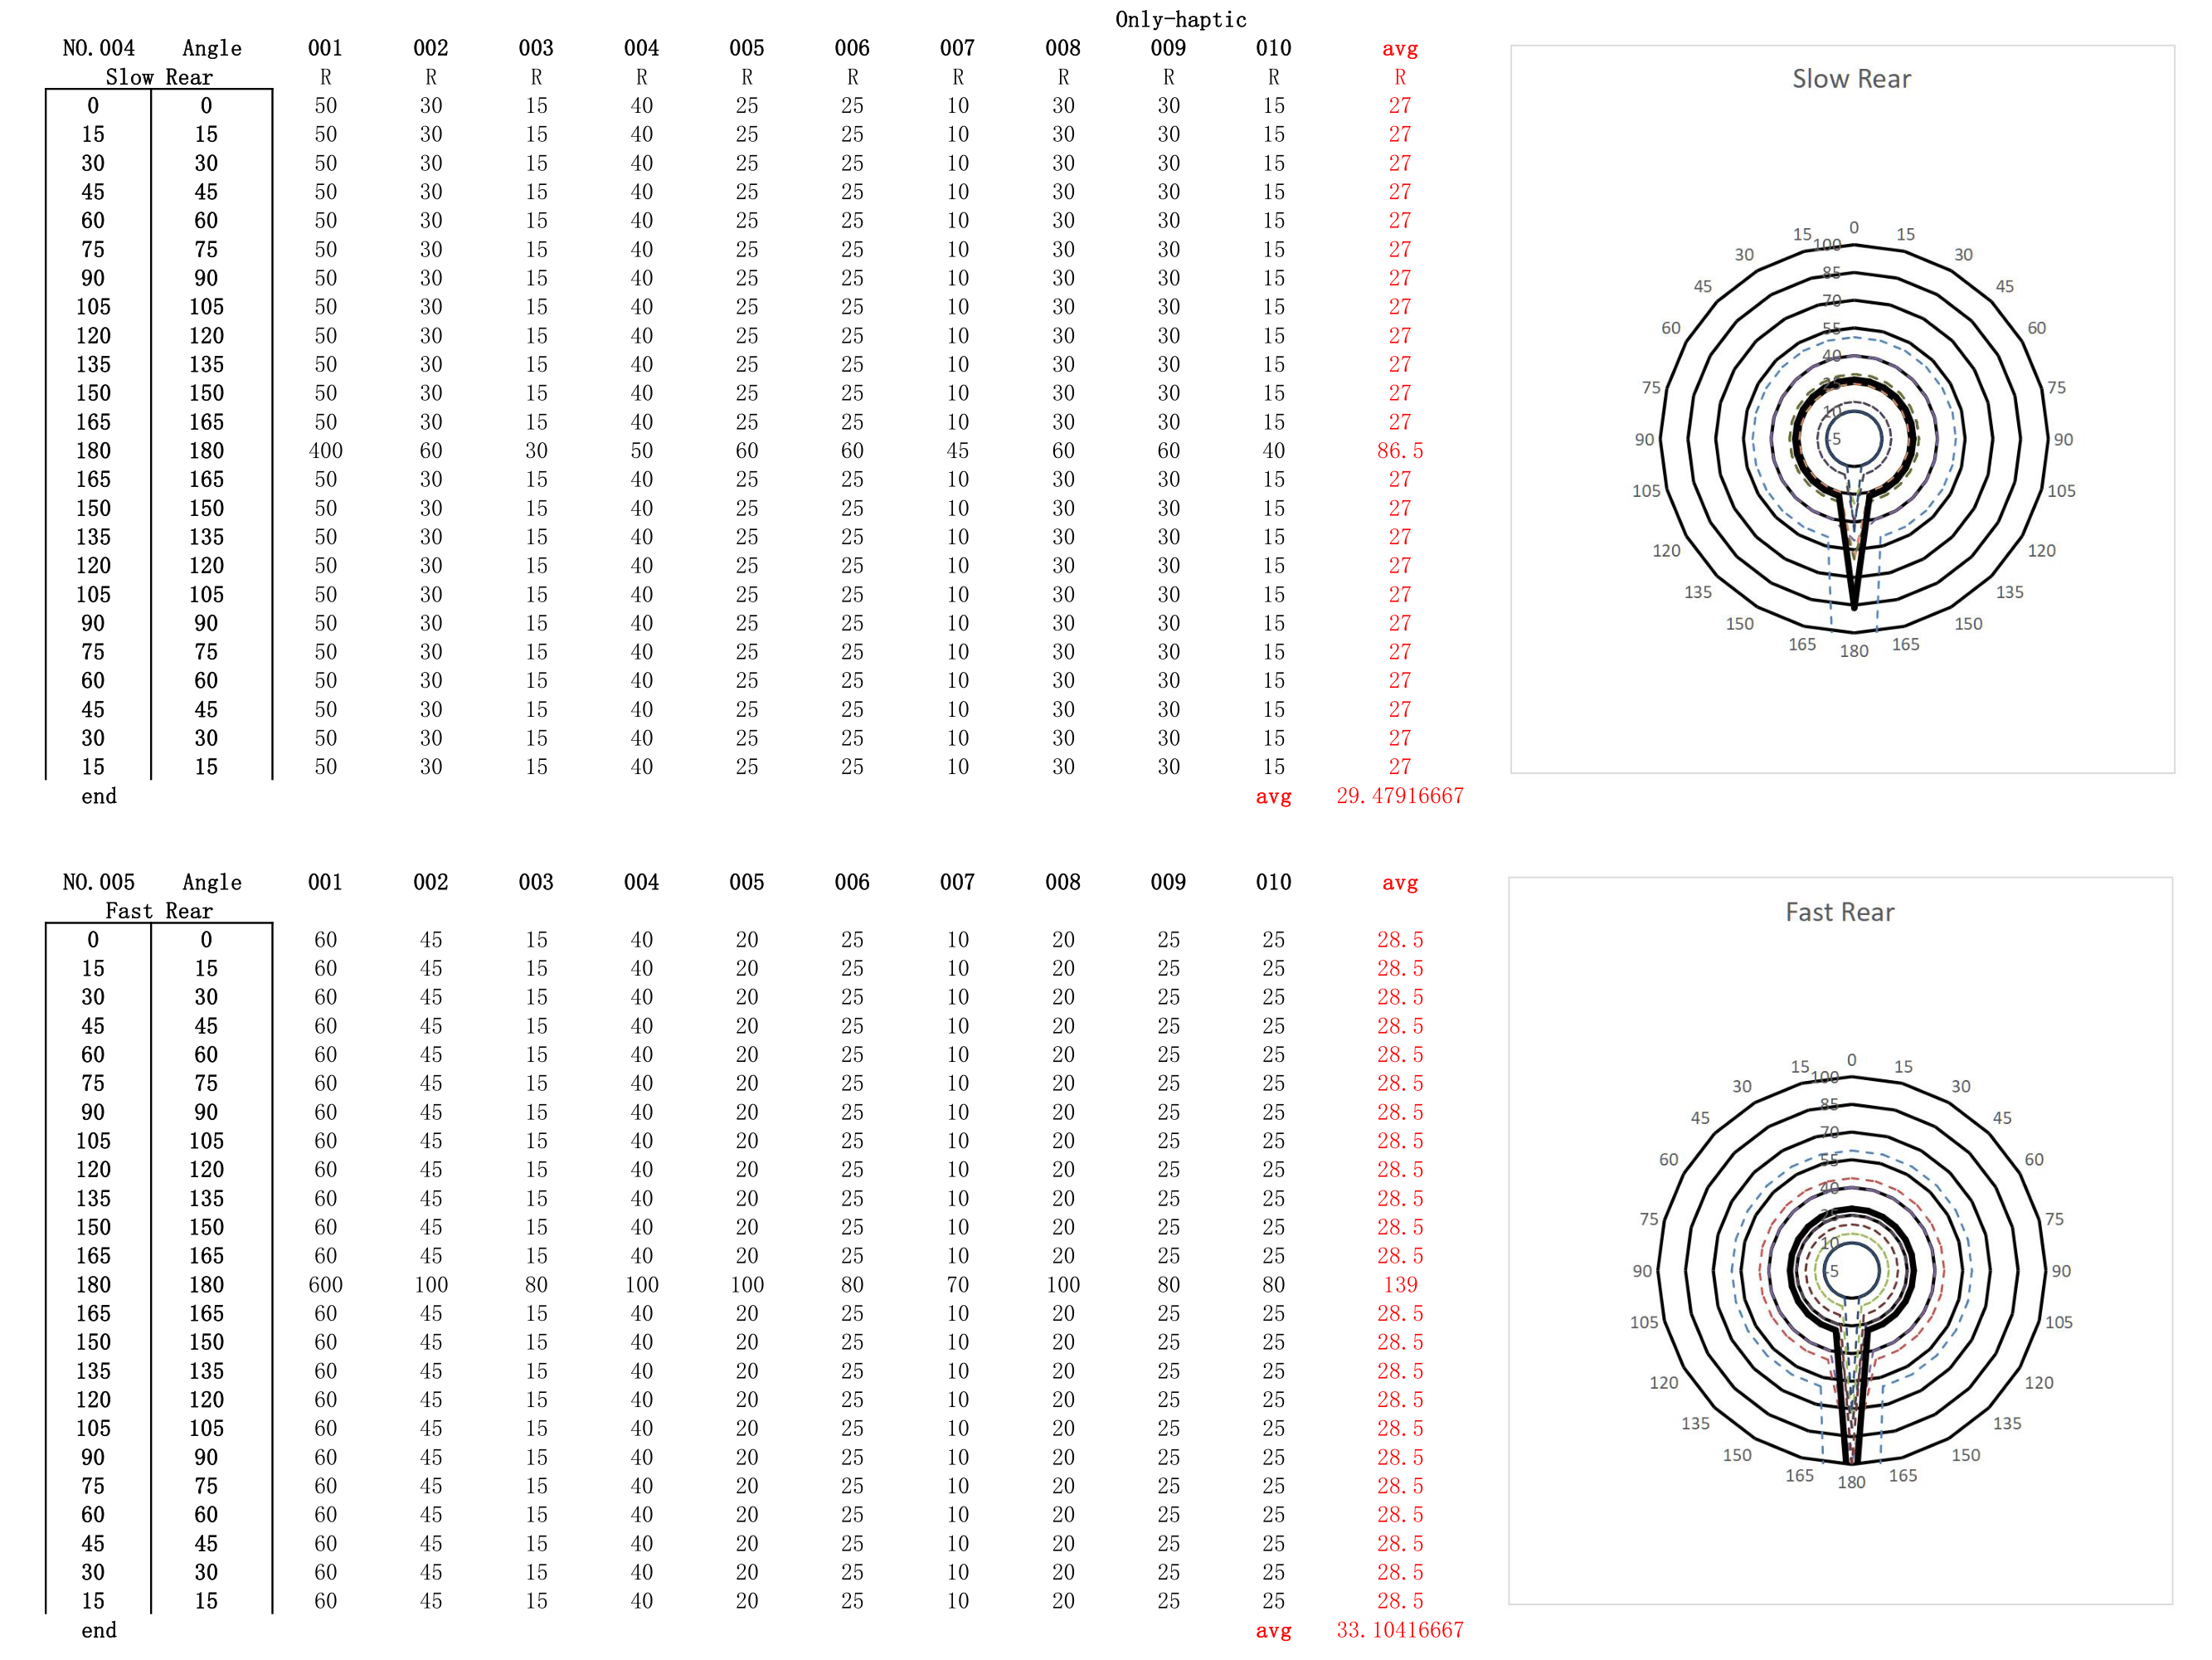
\includegraphics[width=0.9\textwidth,height=0.36\textheight]{A_thesis/appendix/Exp1_1-06.png}
\end{figure}
\newpage

\begin{figure}[h]
\centering
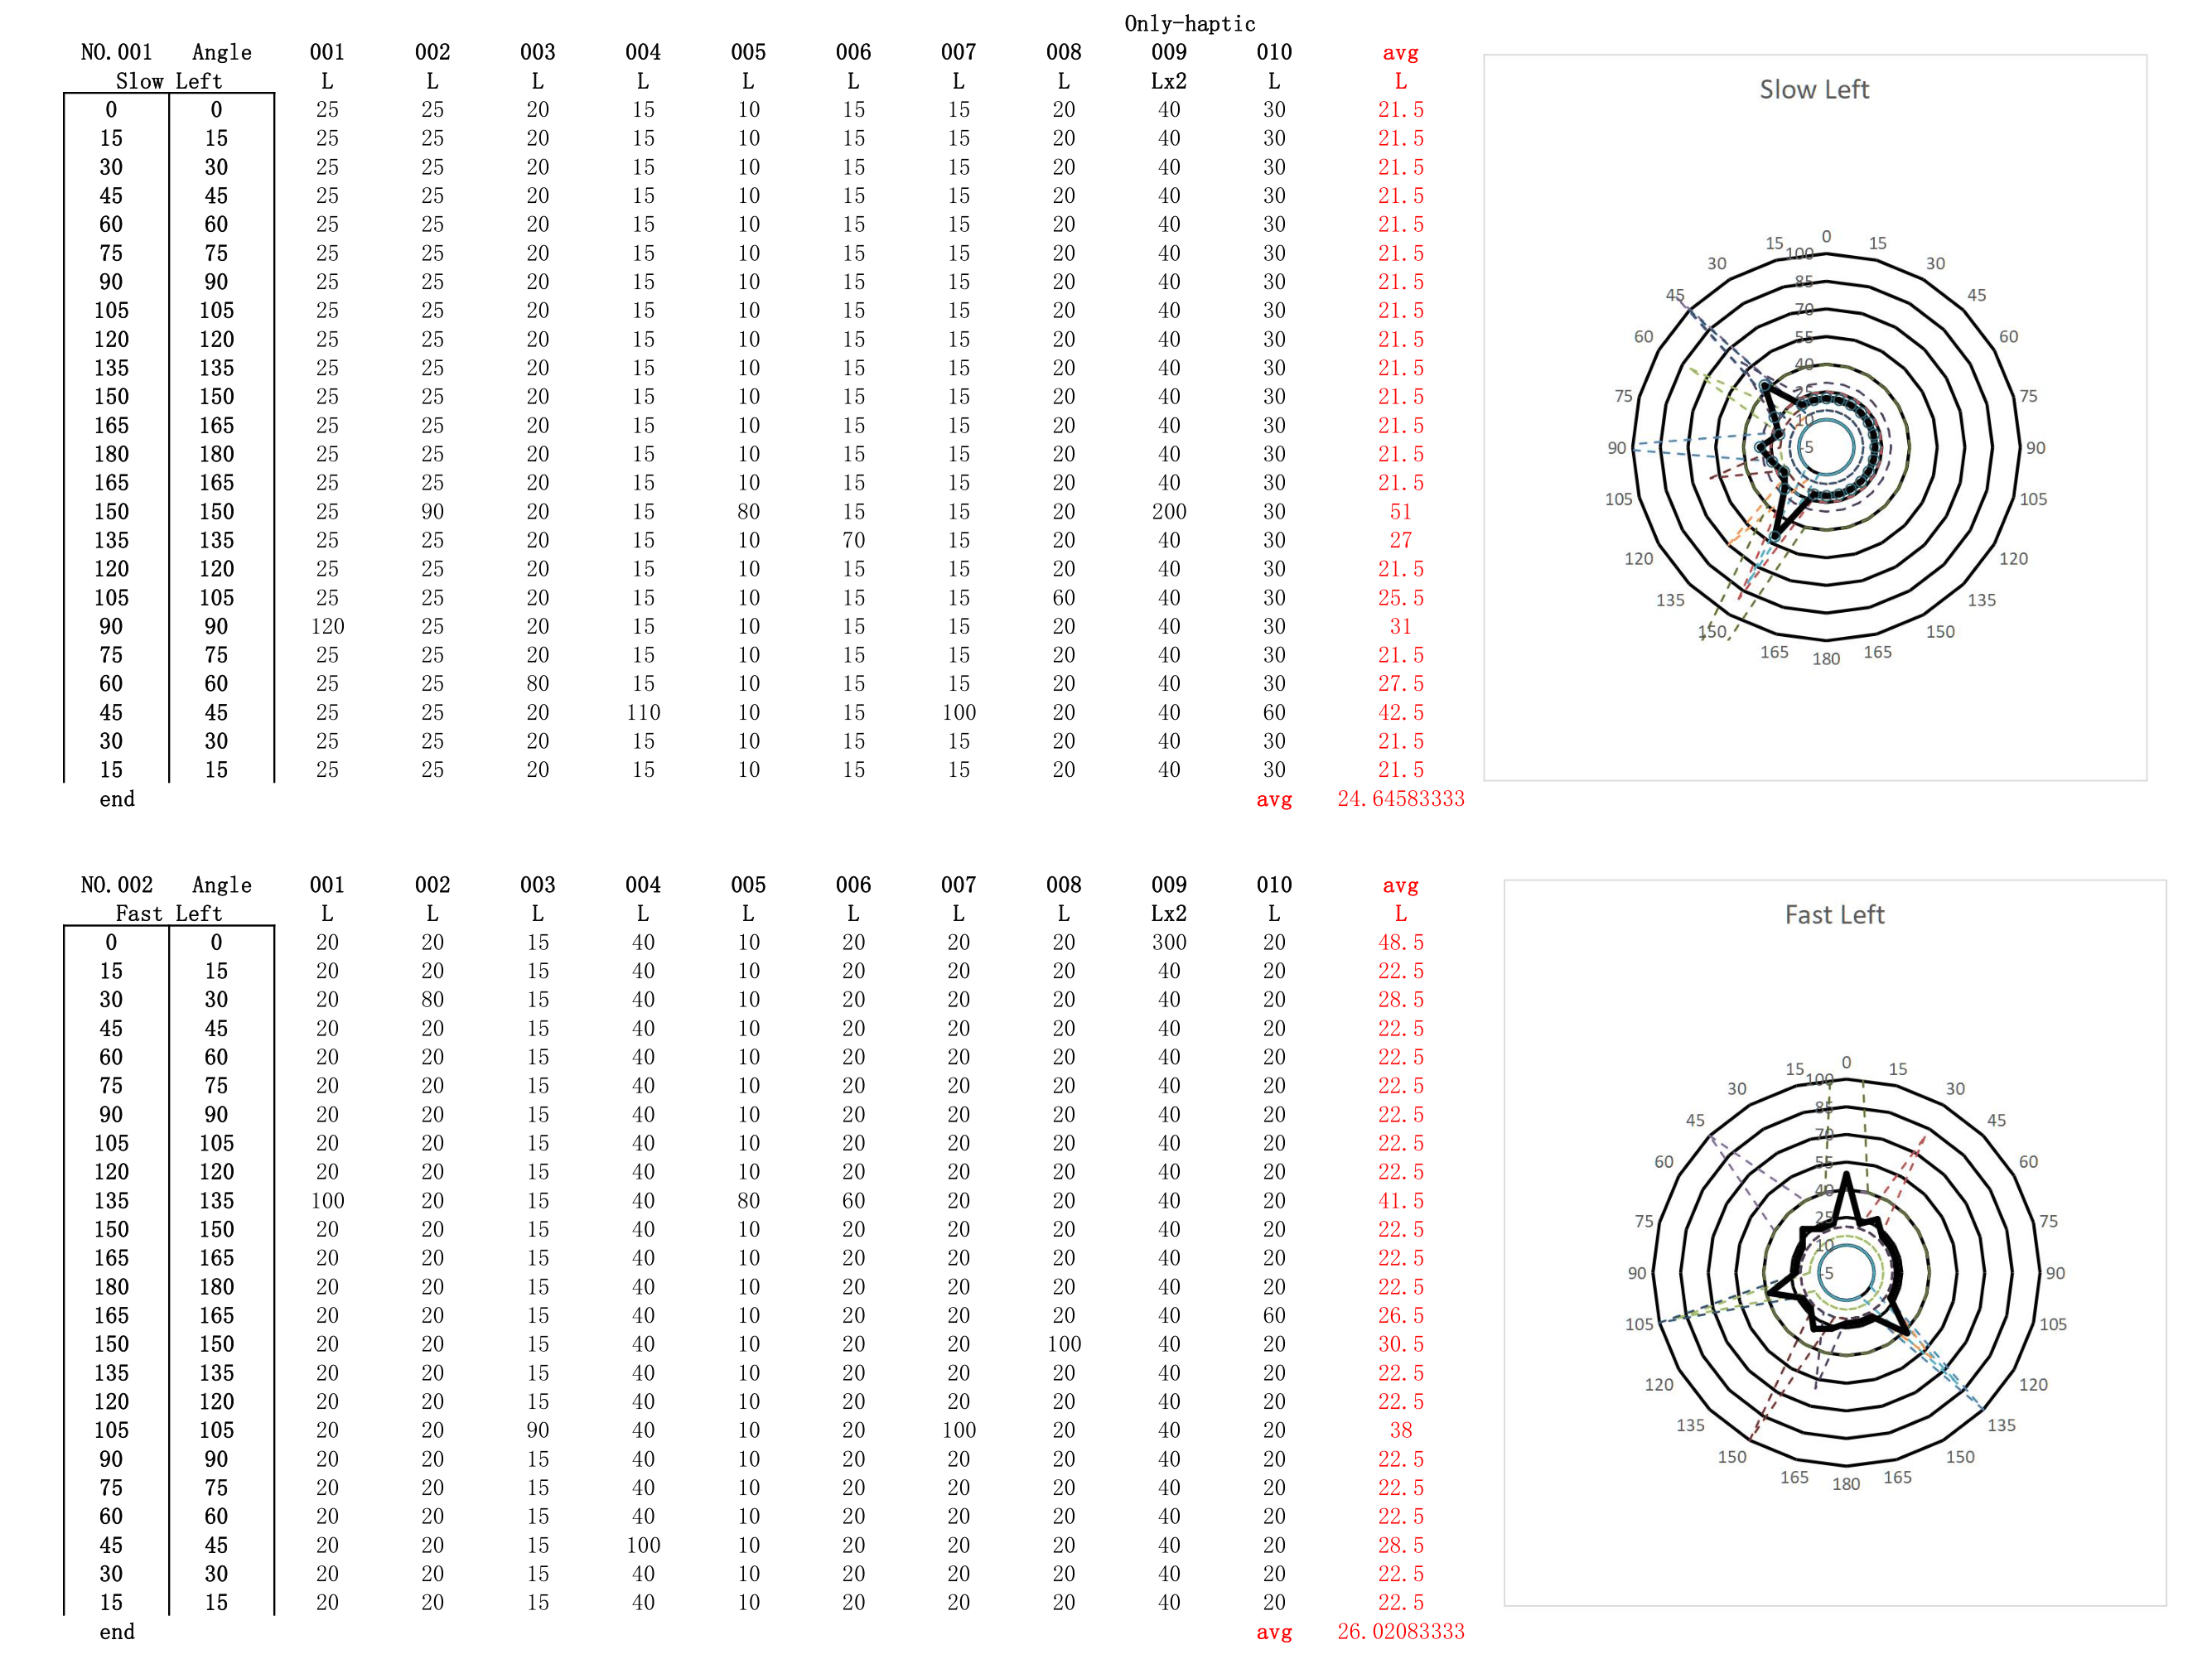
\includegraphics[width=0.9\textwidth,height=0.36\textheight]{A_thesis/appendix/Exp1_1-07.png}
\break
\break
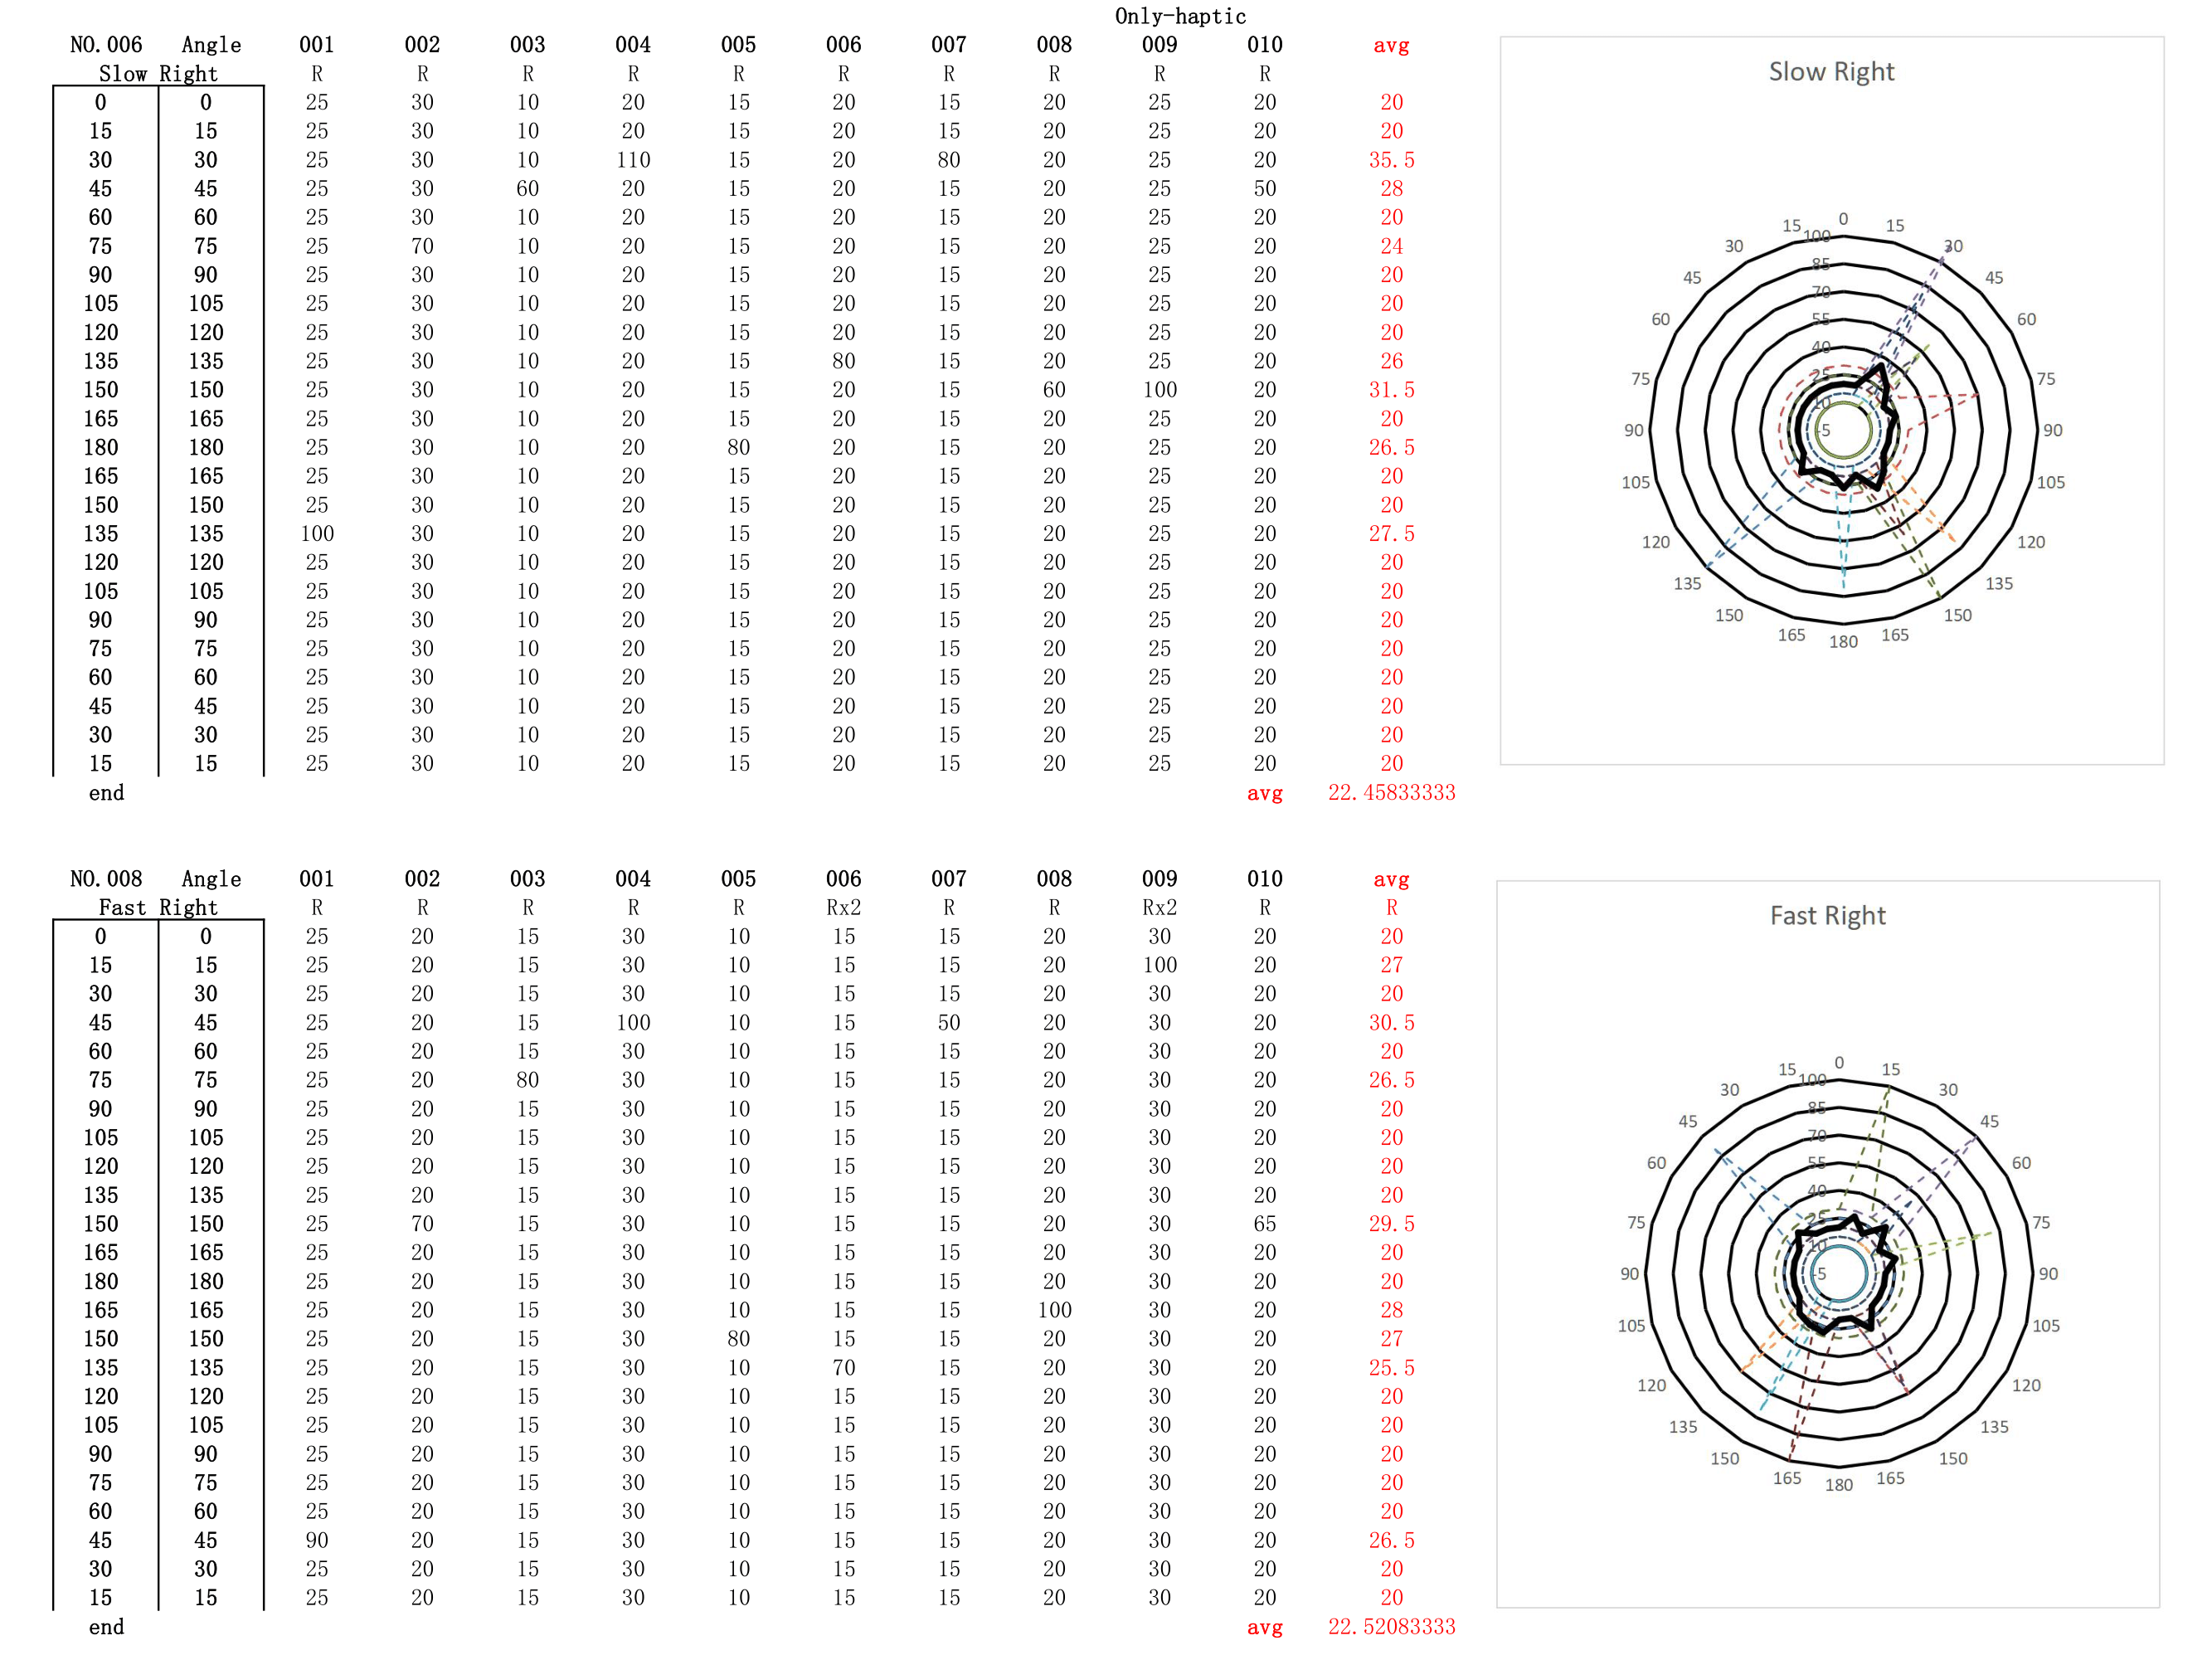
\includegraphics[width=0.9\textwidth,height=0.36\textheight]{A_thesis/appendix/Exp1_1-08.png}
\end{figure}
\newpage

\begin{figure}[h]
\centering
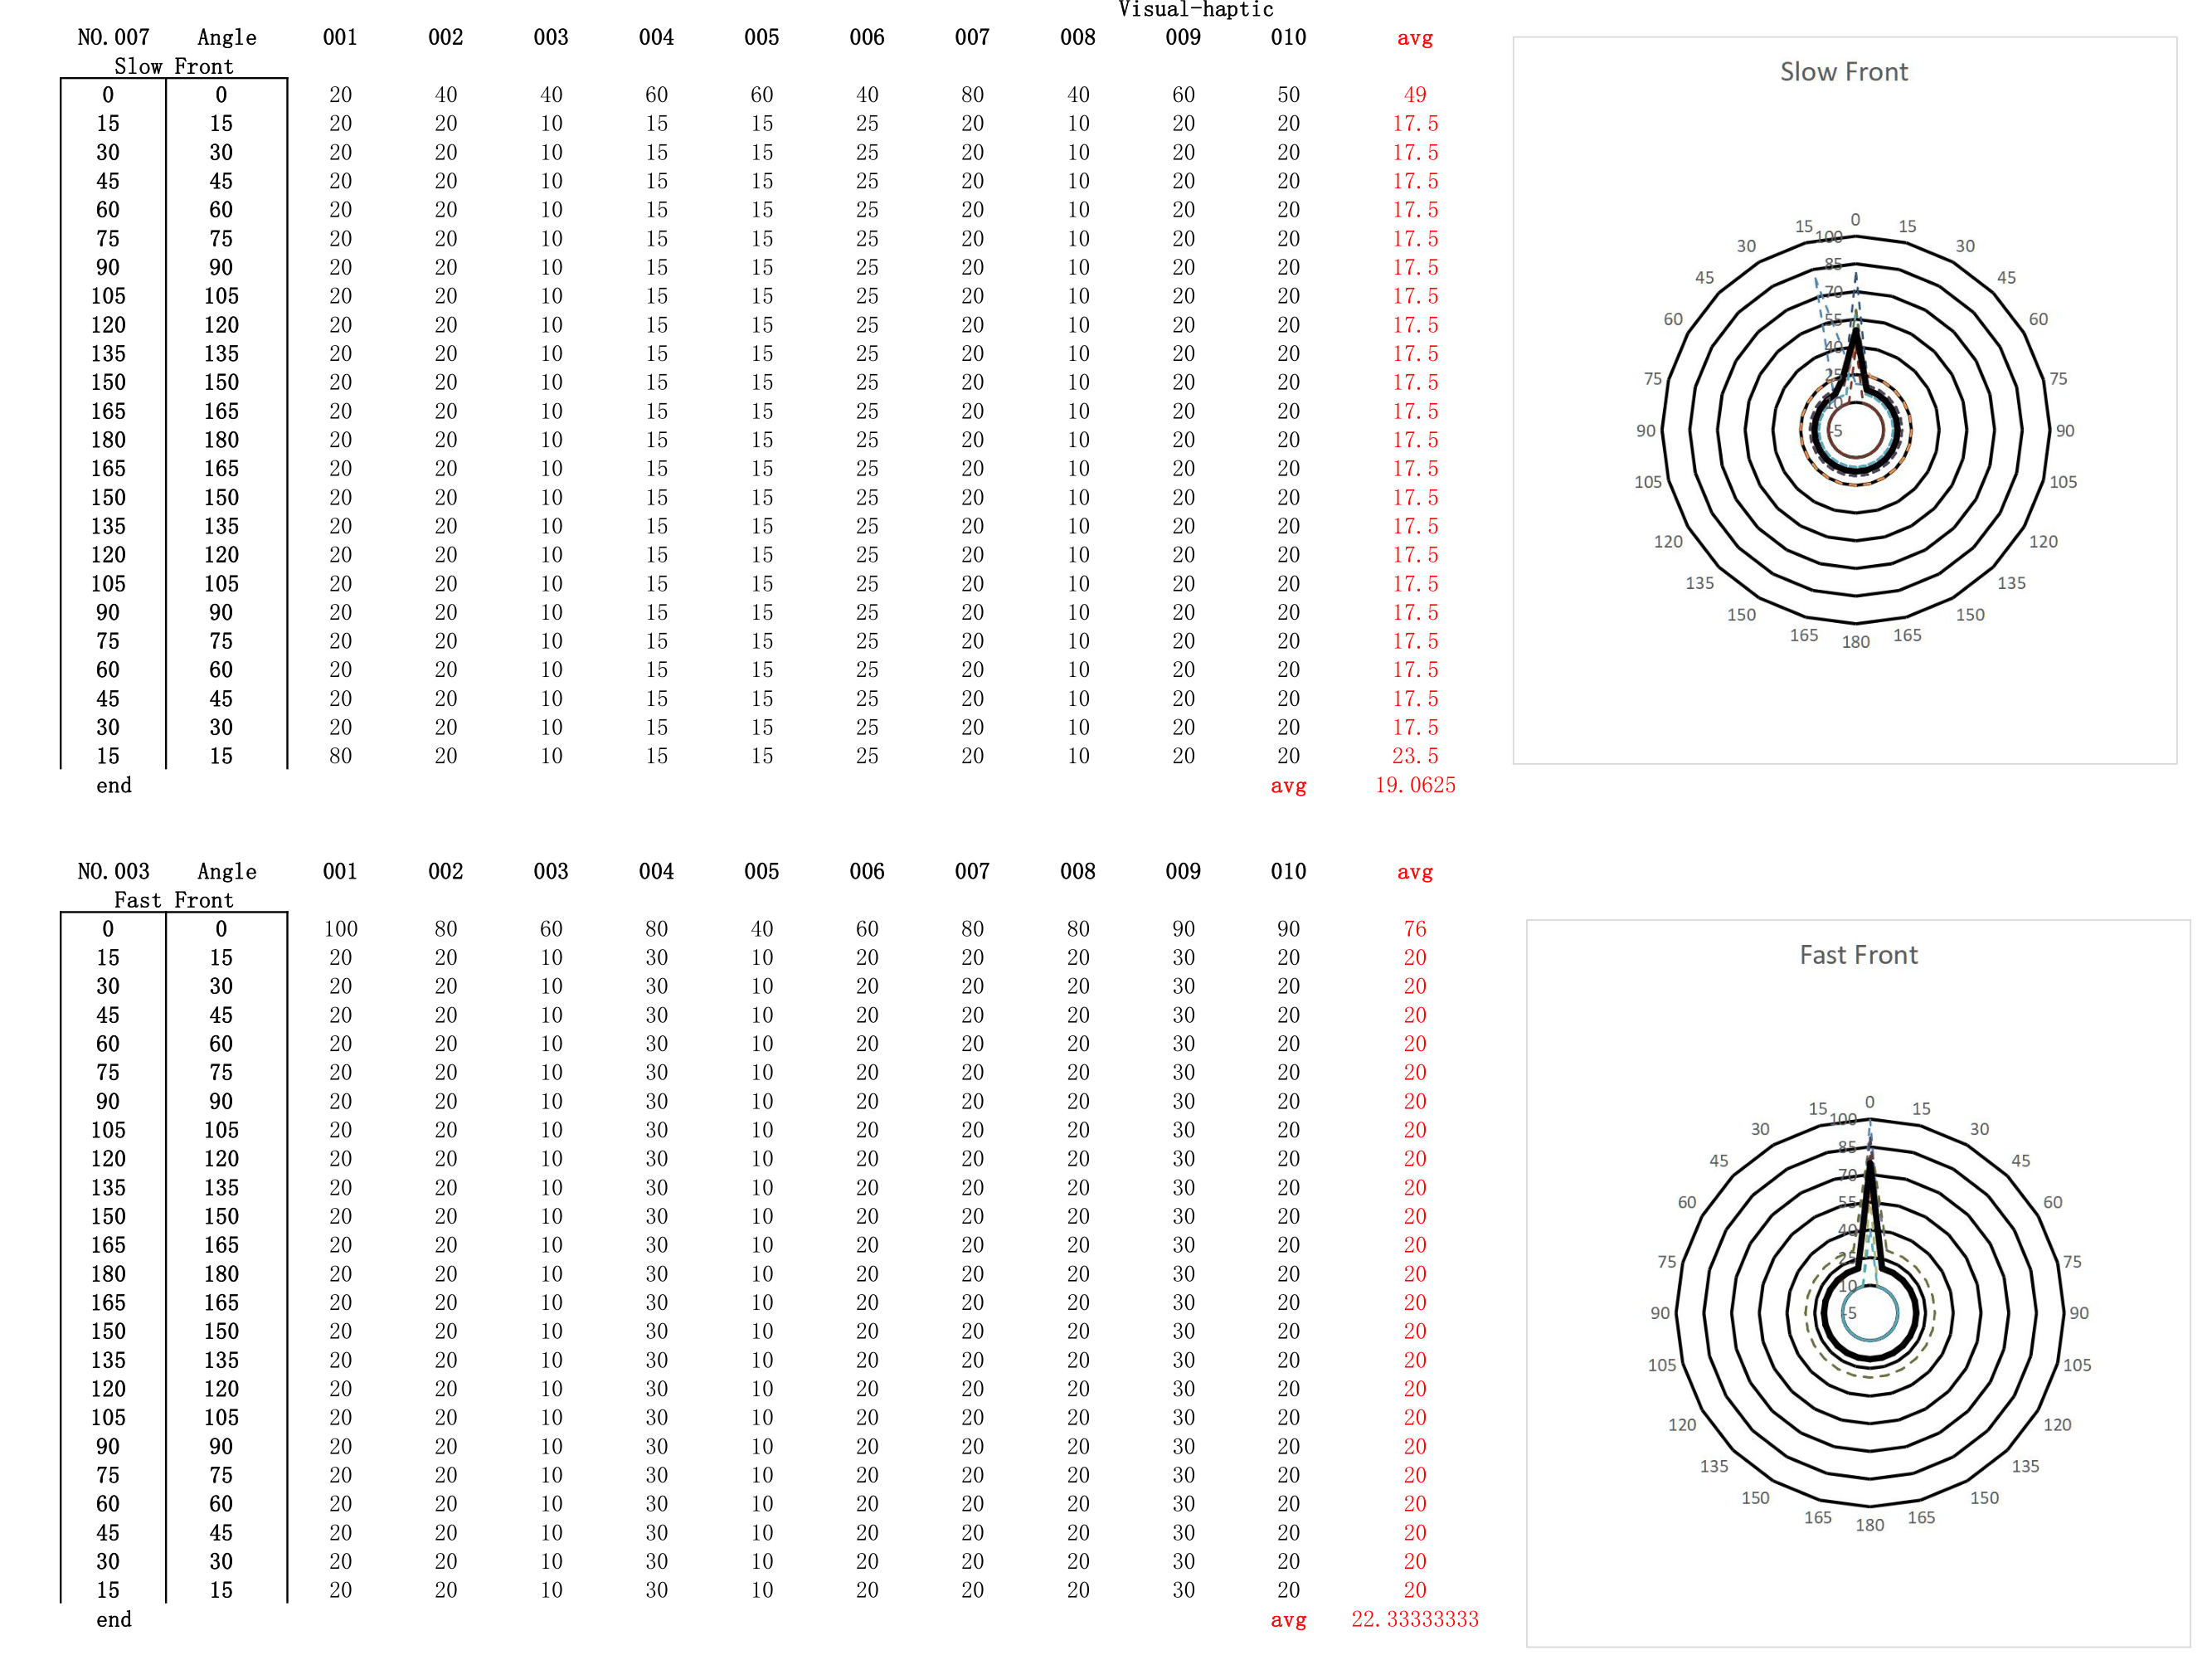
\includegraphics[width=0.9\textwidth,height=0.36\textheight]{A_thesis/appendix/Exp1_1-09.png}
\break
\break
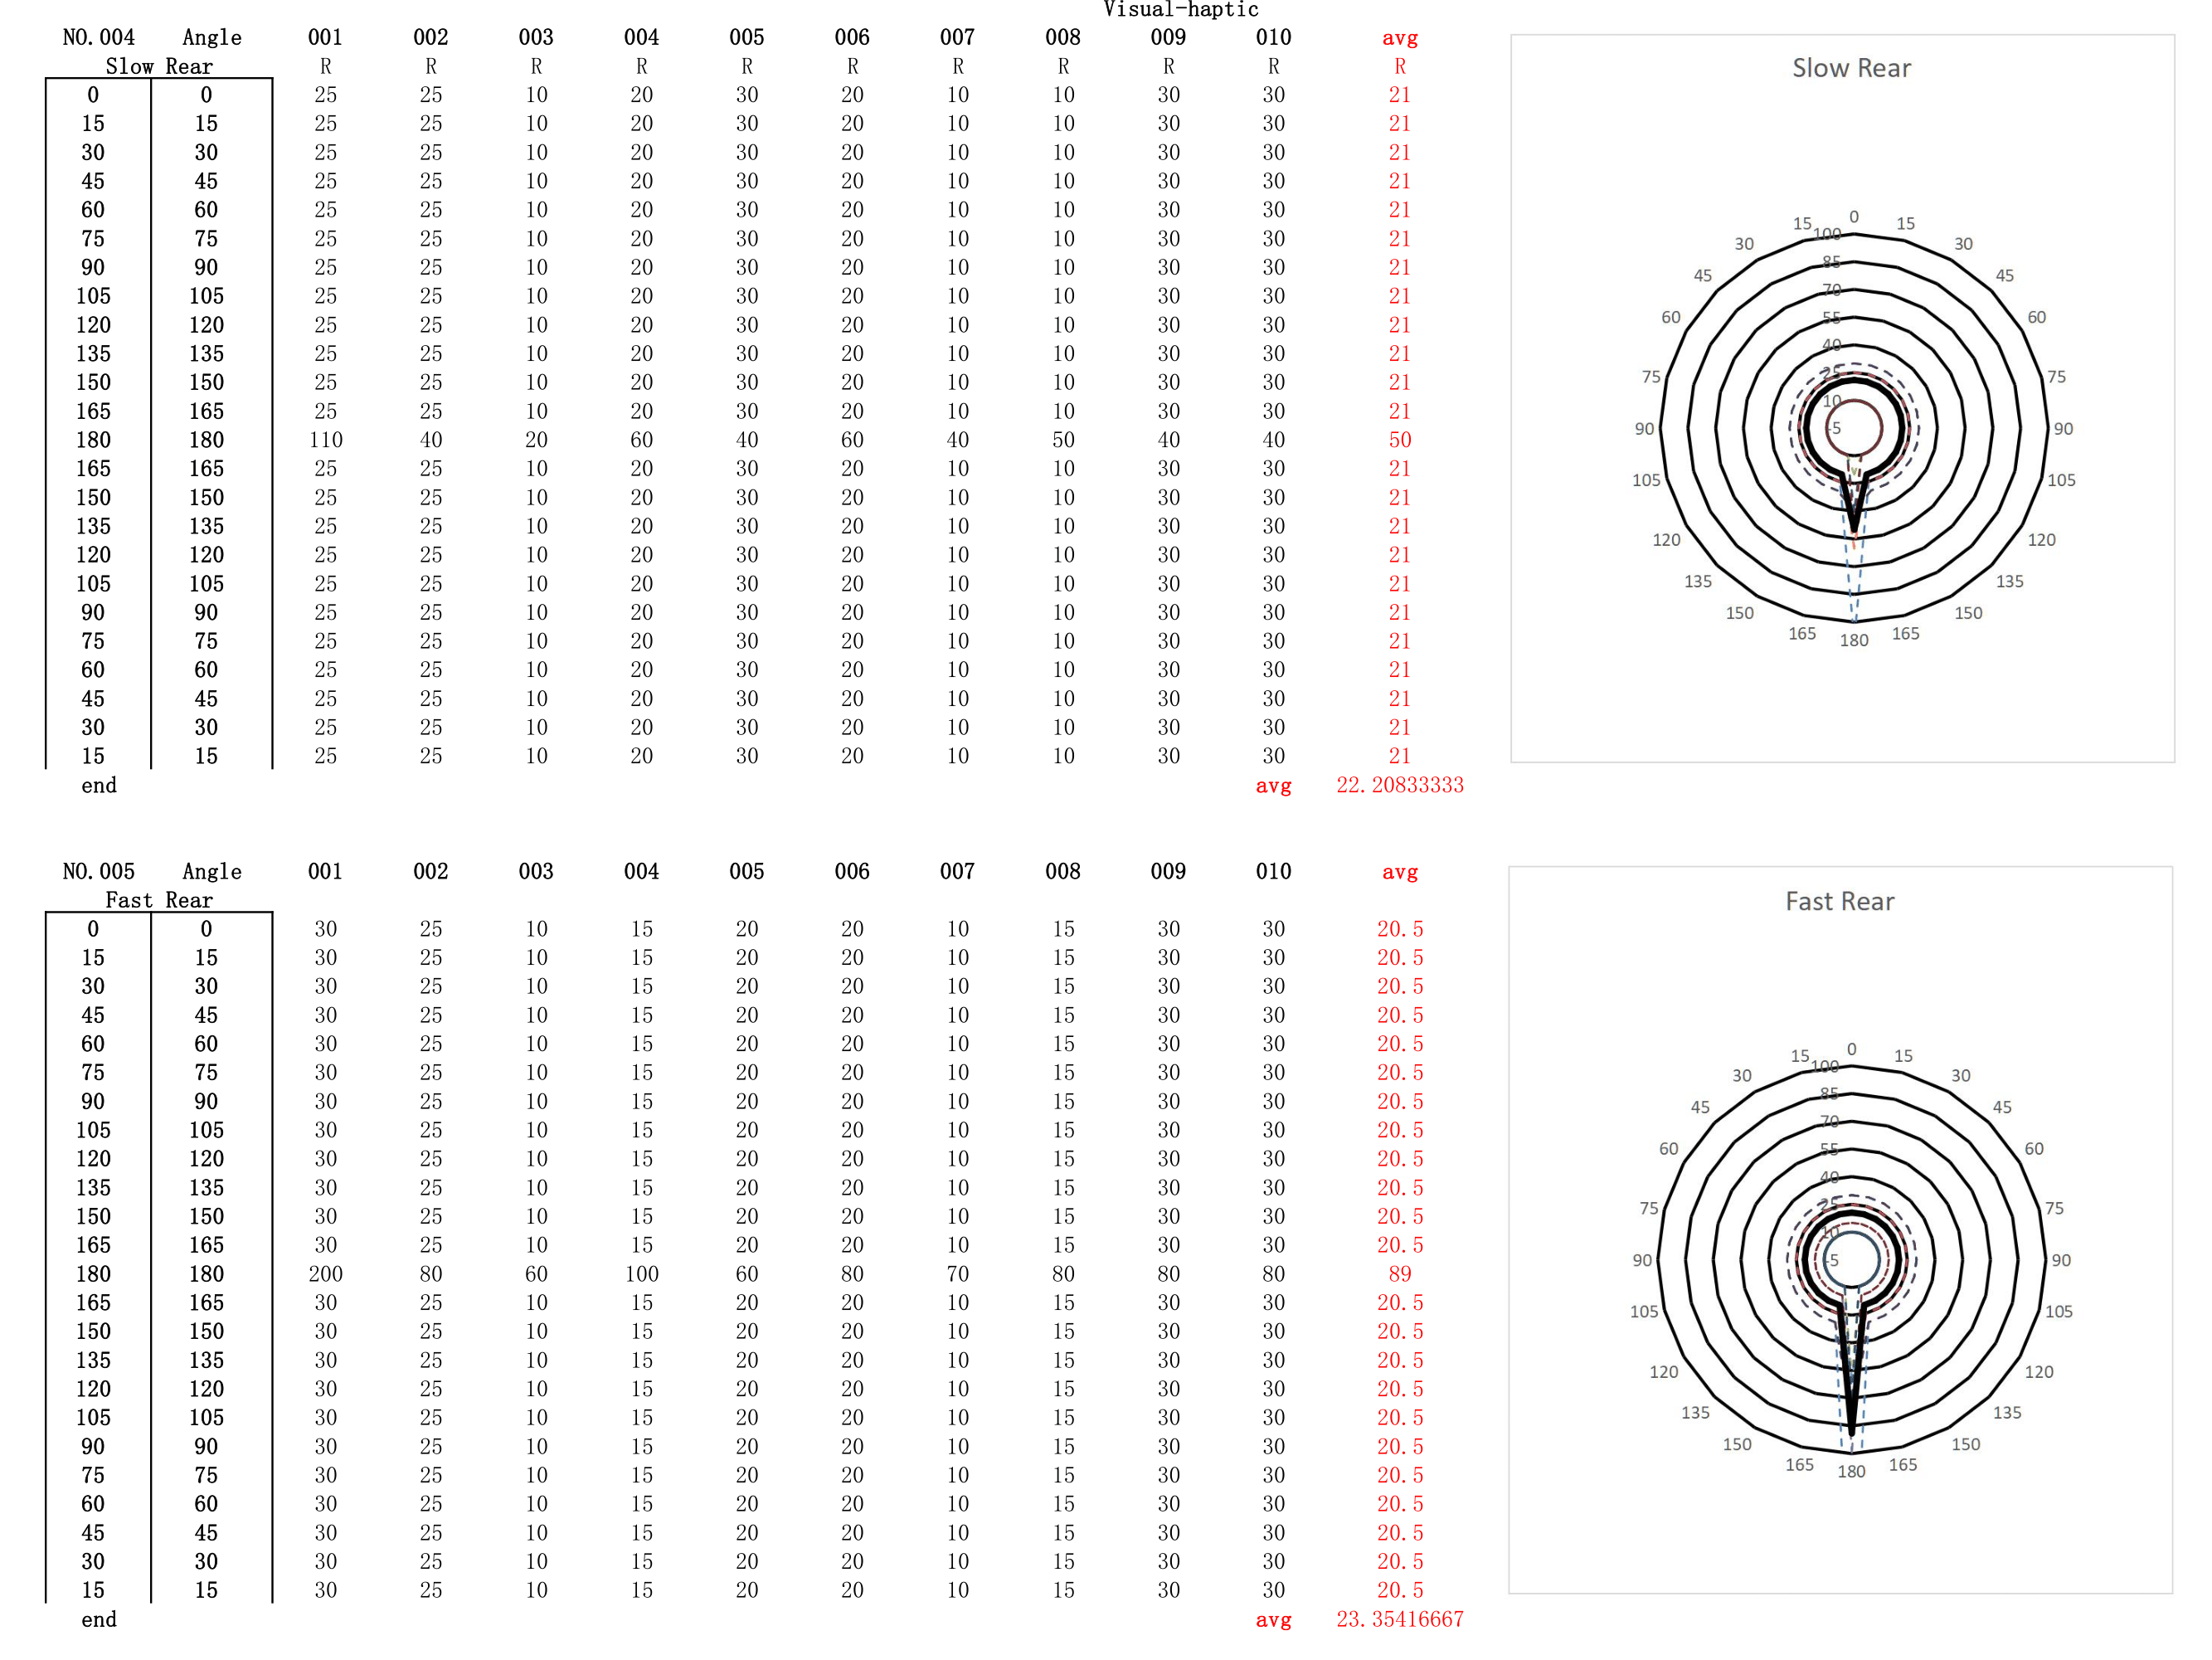
\includegraphics[width=0.9\textwidth,height=0.36\textheight]{A_thesis/appendix/Exp1_1-10.png}
\end{figure}
\newpage

\begin{figure}[h]
\centering
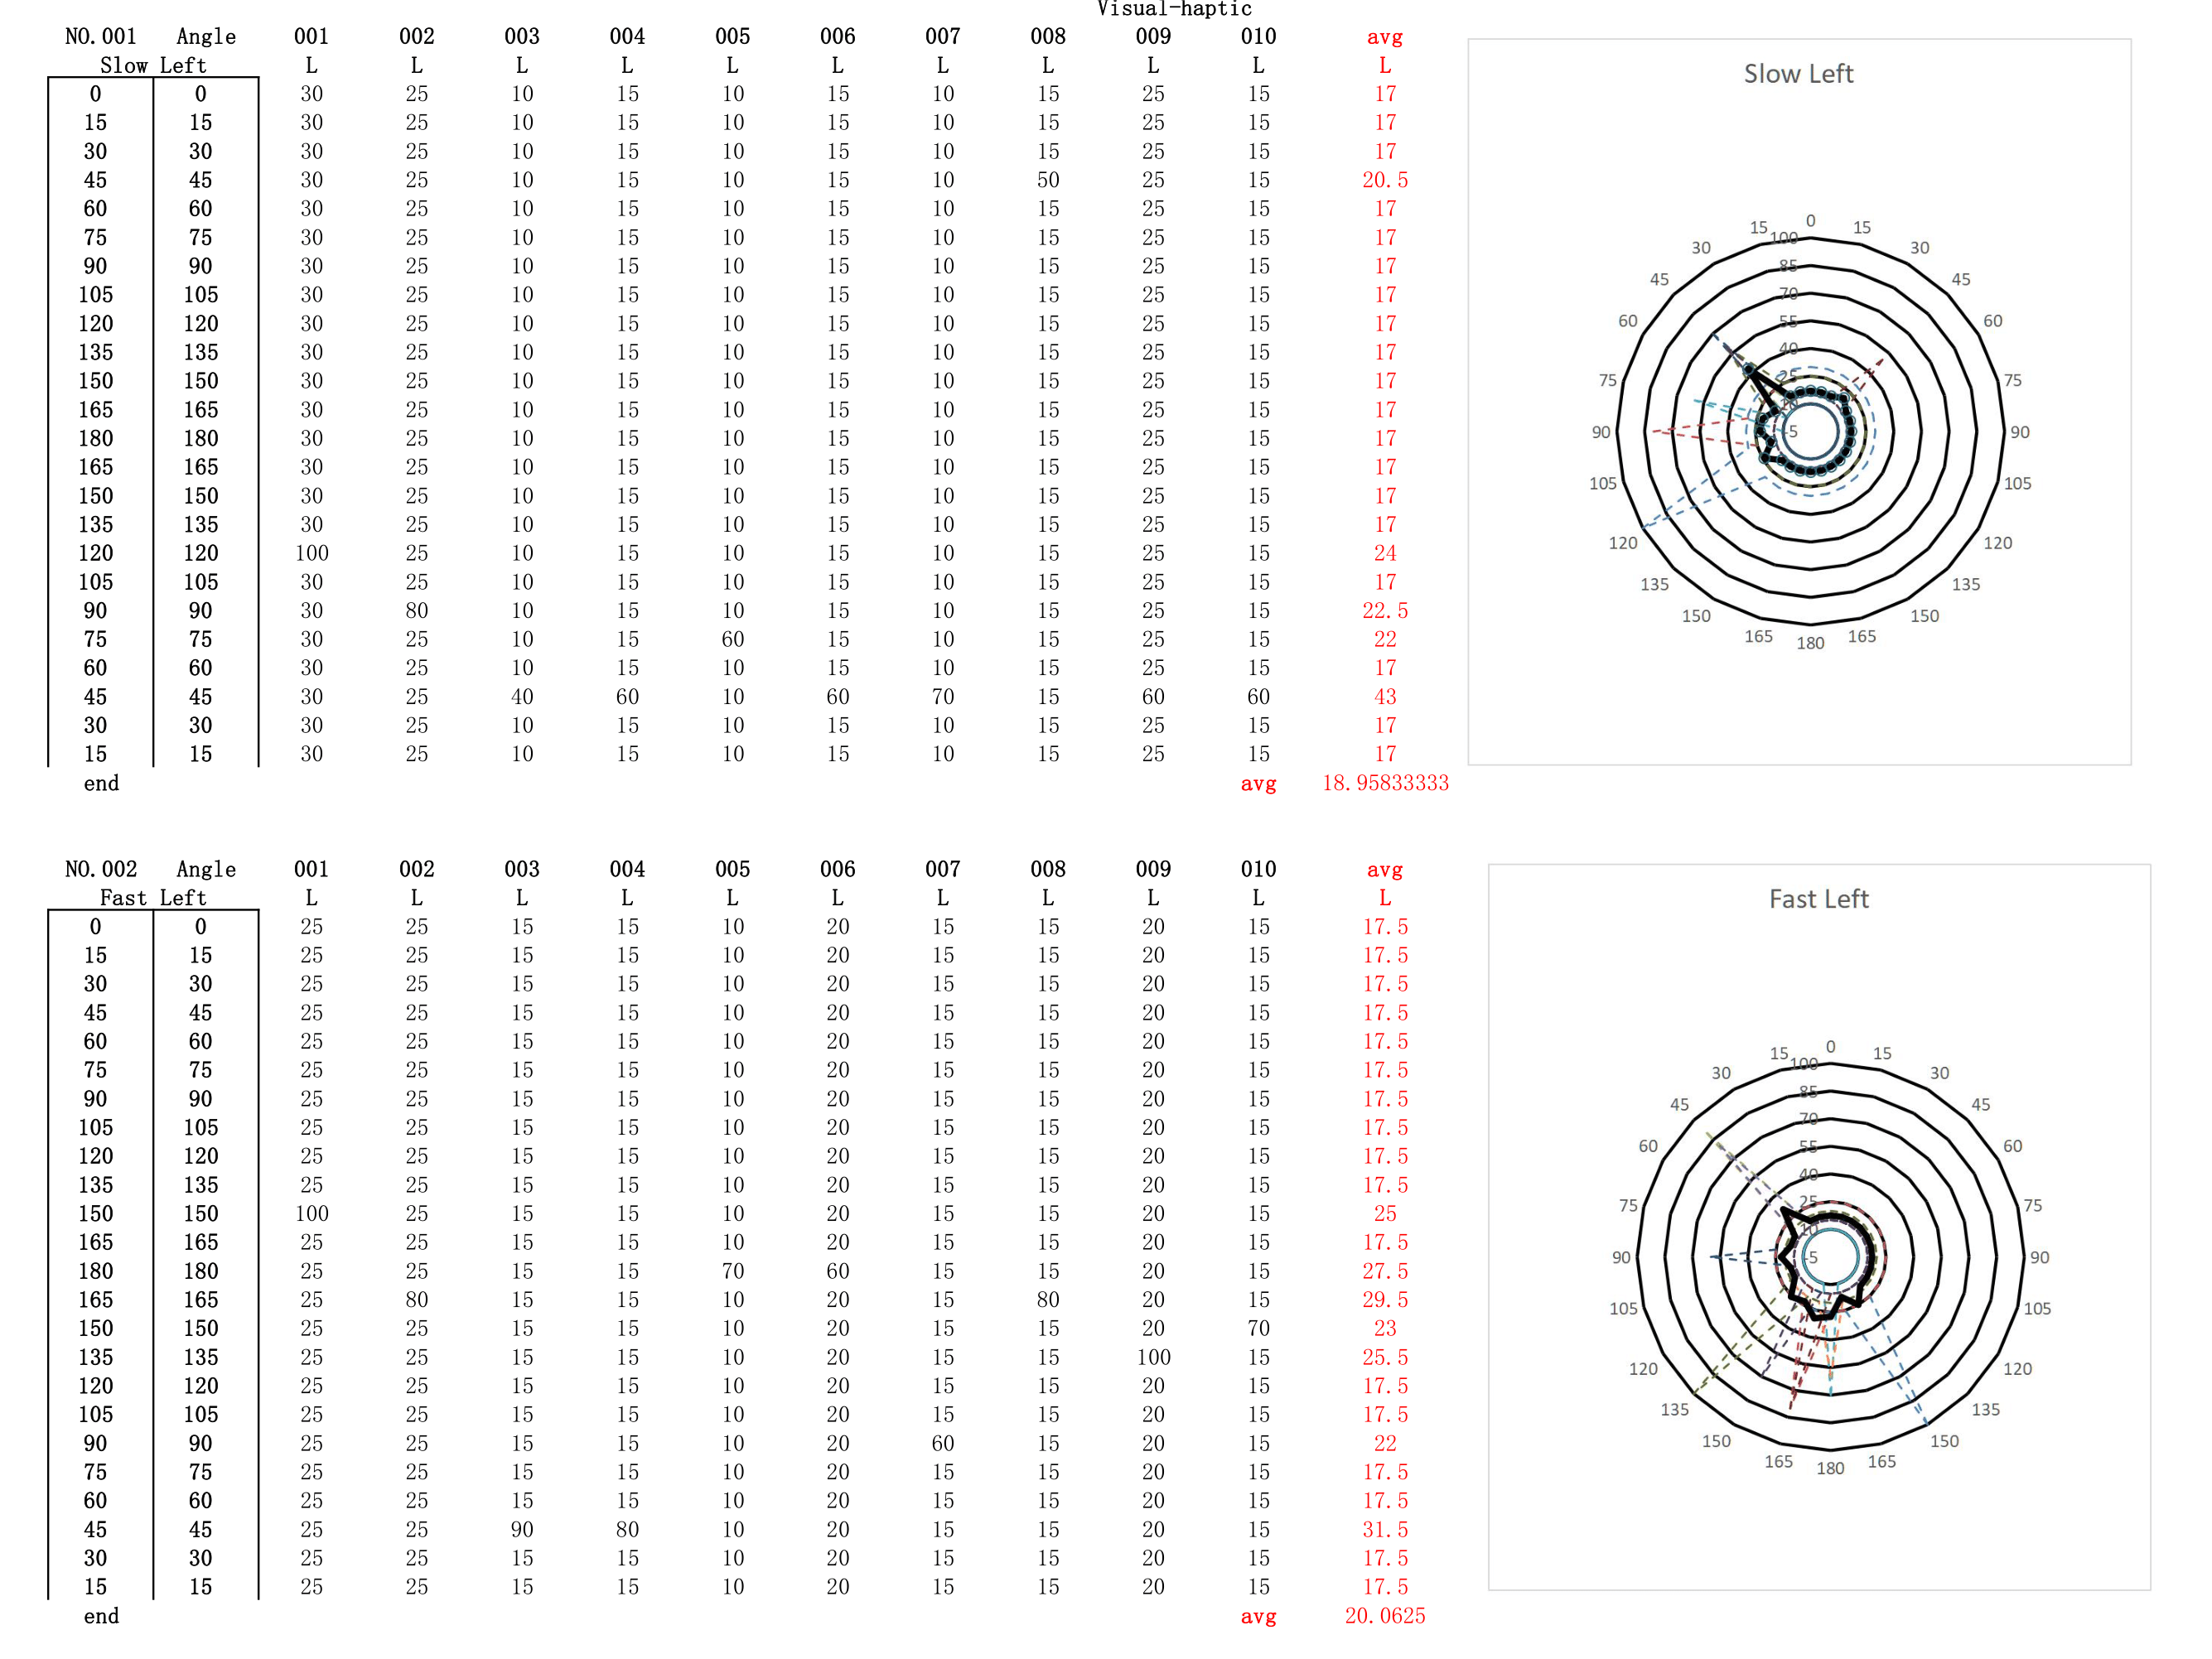
\includegraphics[width=0.9\textwidth,height=0.36\textheight]{A_thesis/appendix/Exp1_1-11.png}
\break
\break
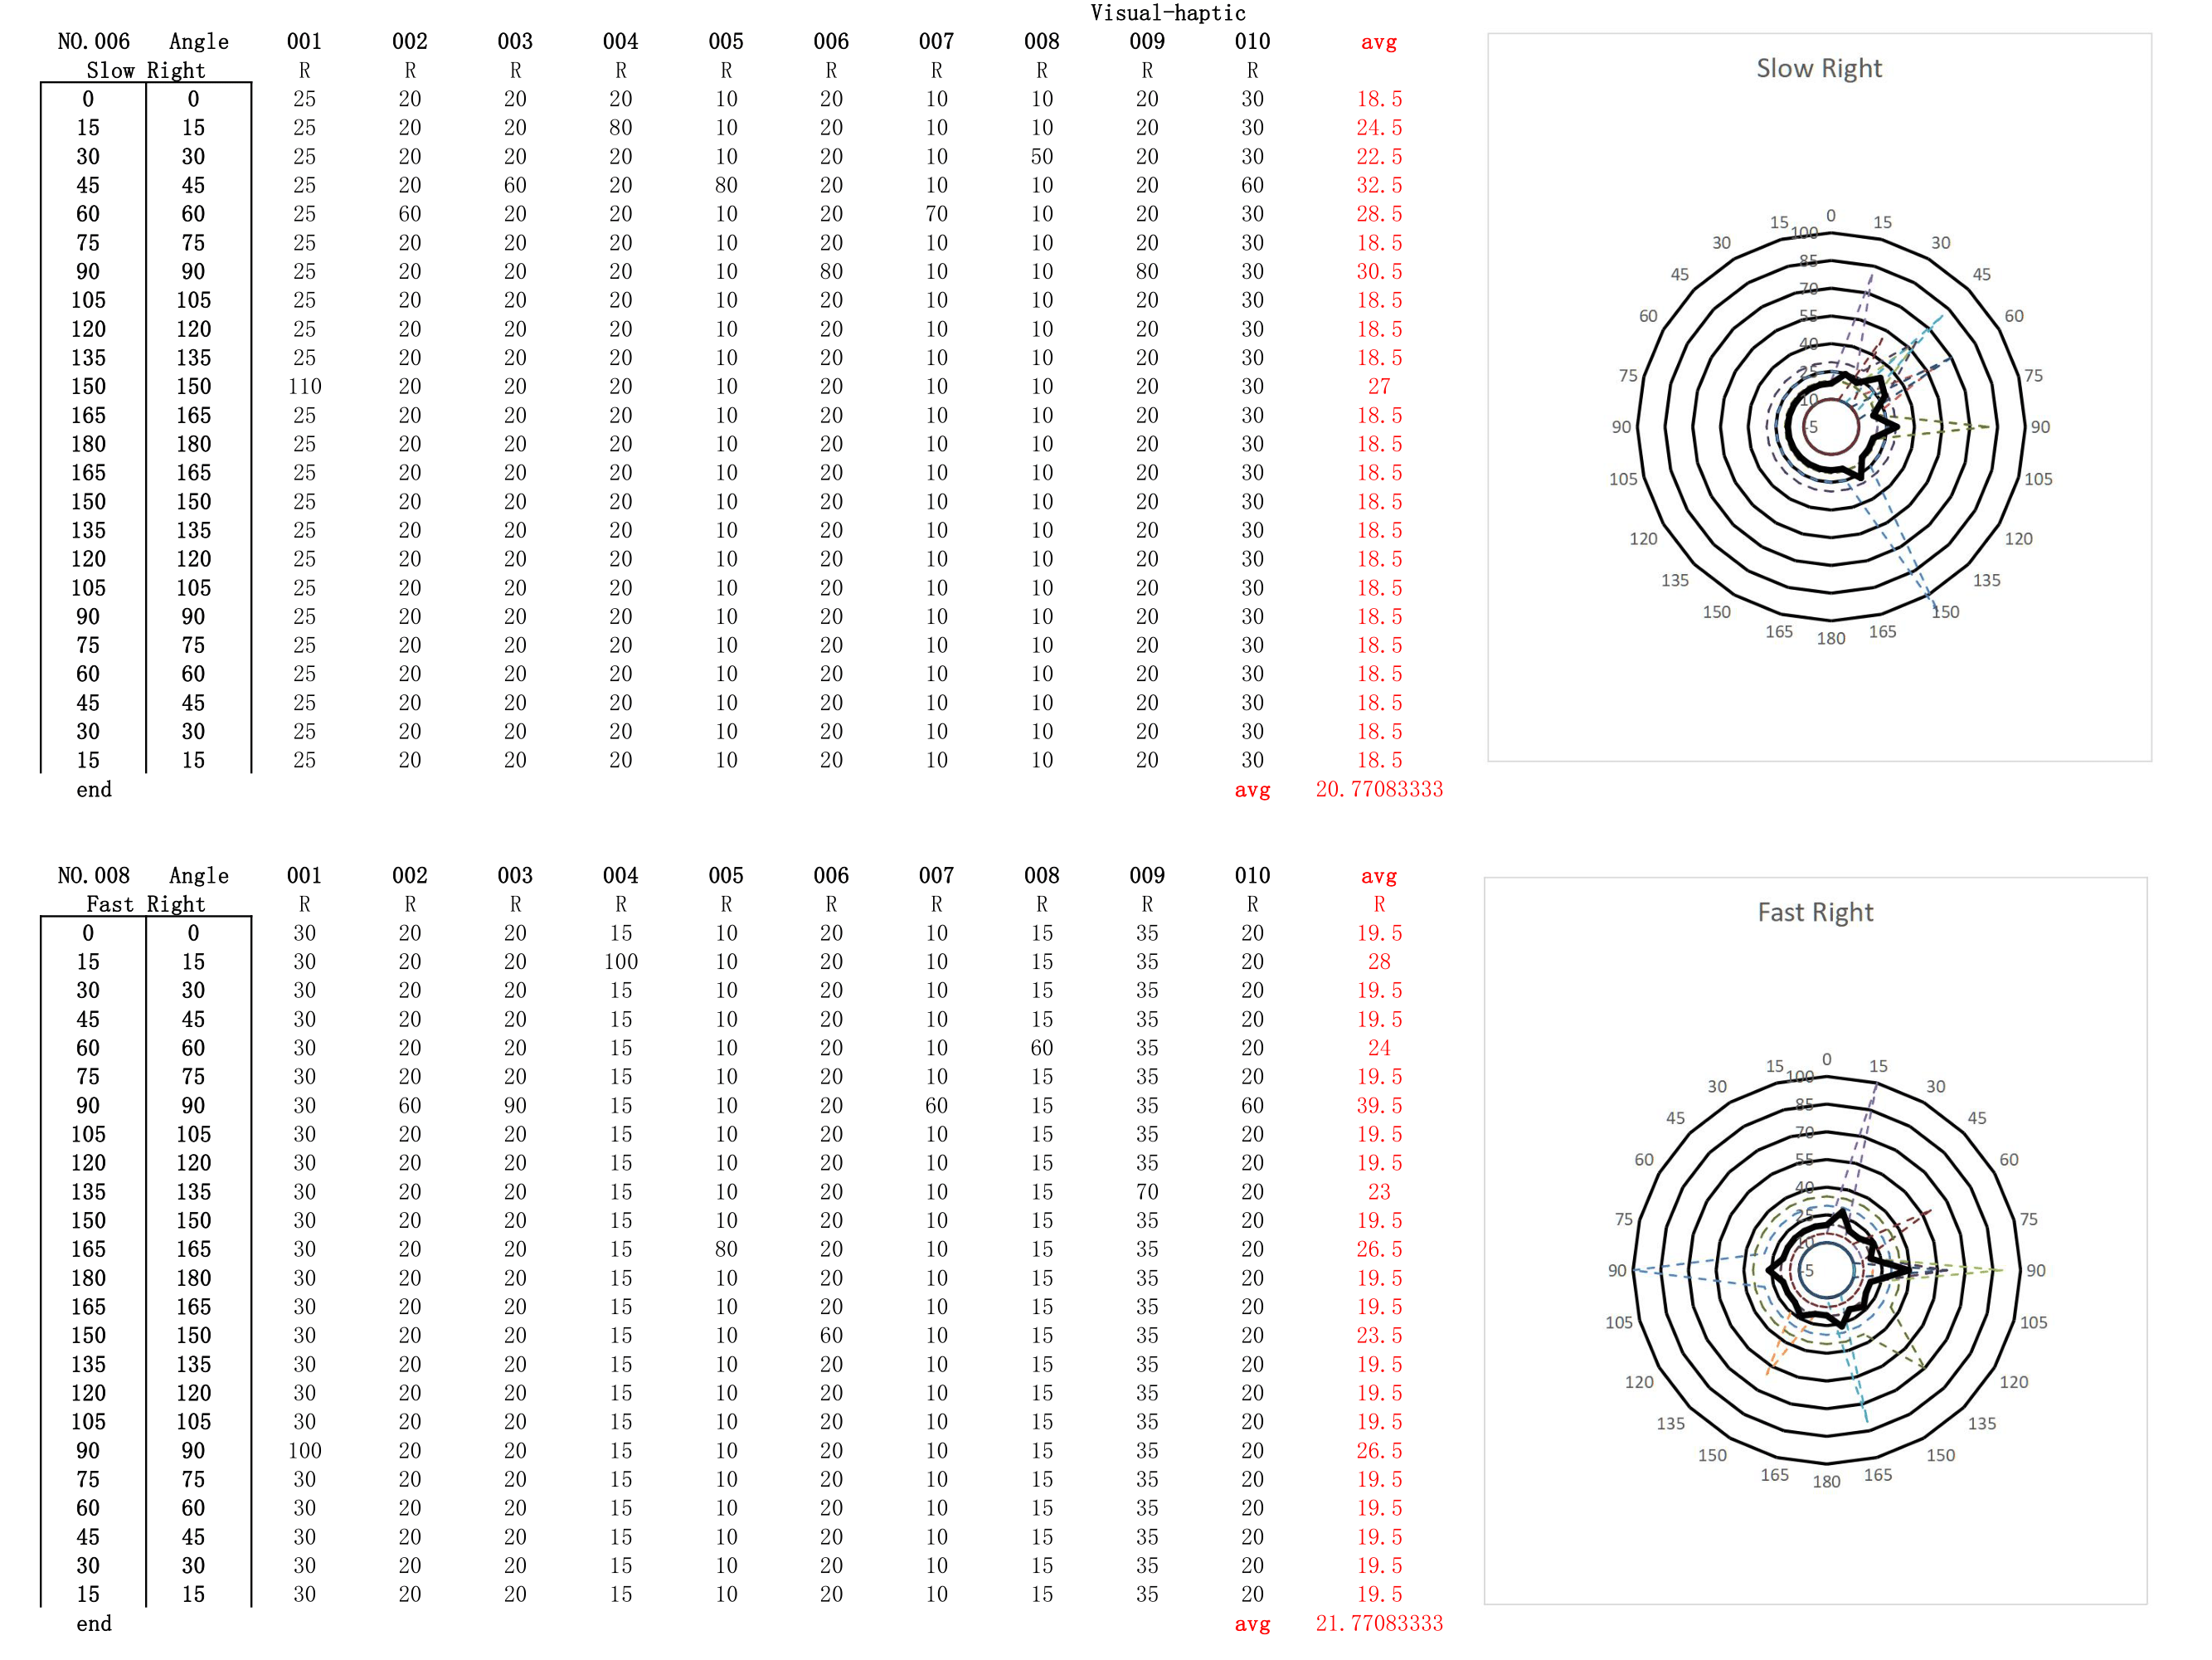
\includegraphics[width=0.9\textwidth,height=0.36\textheight]{A_thesis/appendix/Exp1_1-12.png}
\end{figure}
\newpage

\section{Questionnaire Result}
\begin{figure}[h]
\centering
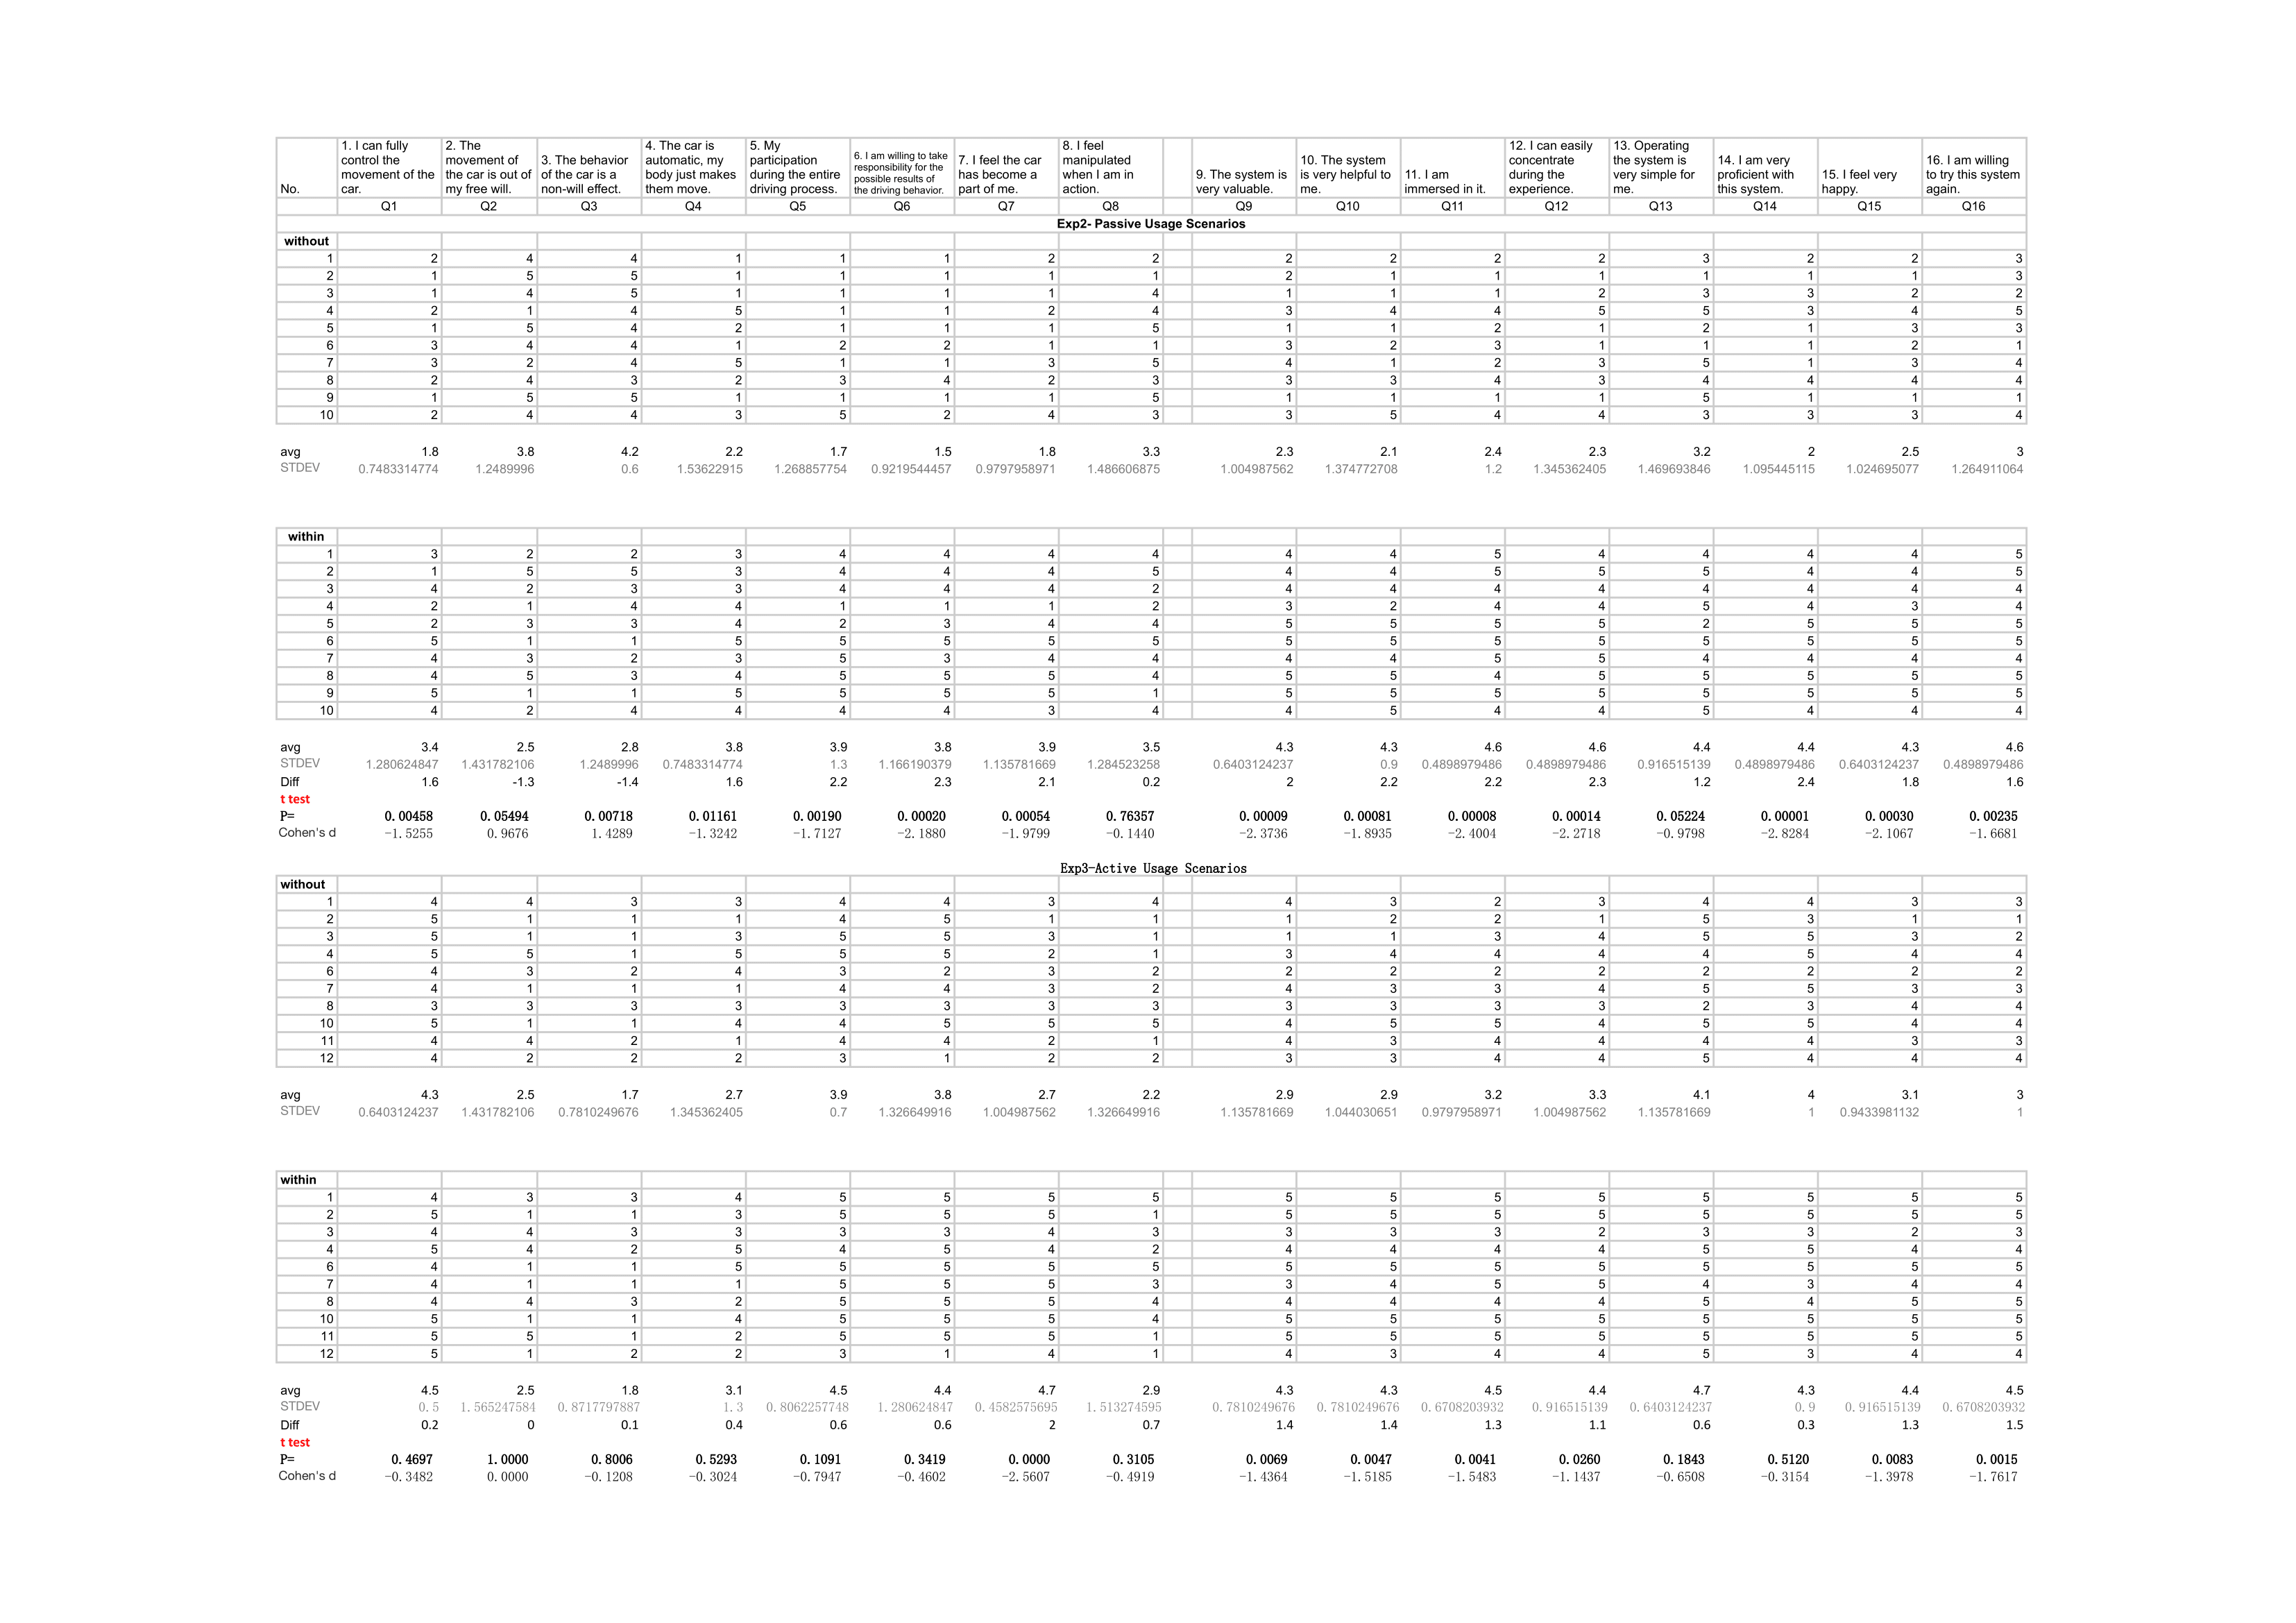
\includegraphics[width=1\textwidth,height=0.75\textheight]{A_thesis/appendix/Analysis2 3.xlsx - Exp23-1.png}
\end{figure}


